%% 
%% Copyright 2019-2021 Elsevier Ltd
%% 
%% This file is part of the 'CAS Bundle'.
%% --------------------------------------
%% 
%% It may be distributed under the conditions of the LaTeX Project Public
%% License, either version 1.2 of this license or (at your option) any
%% later version.  The latest version of this license is in
%%    http://www.latex-project.org/lppl.txt
%% and version 1.2 or later is part of all distributions of LaTeX
%% version 1999/12/01 or later.
%% 
%% The list of all files belonging to the 'CAS Bundle' is
%% given in the file `manifest.txt'.
%% 
%% Template article for cas-sc documentclass for 
%% single column output.

\documentclass[a4paper,fleqn]{cas-sc}

% If the frontmatter runs over more than one page
% use the longmktitle option.

%\documentclass[a4paper,fleqn,longmktitle]{cas-sc}

%\usepackage[numbers]{natbib}
\usepackage[authoryear]{natbib}
% \usepackage[authoryear,longnamesfirst]{natbib}

\usepackage{graphicx}%
\usepackage{multirow}%
\usepackage{amsmath,amssymb,amsfonts}%
\usepackage{amsthm}%
\usepackage{mathrsfs}%
% \usepackage[title]{appendix}%
\usepackage{xcolor}%
\definecolor{citeblue}{RGB}{0,115,185}
\hypersetup{
    colorlinks=true,
    citecolor=citeblue,
    linkcolor=citeblue,
    urlcolor=citeblue
}
\usepackage{textcomp}%
\usepackage{manyfoot}%
\usepackage{booktabs}%
\usepackage{algorithm}
\usepackage{algorithmic}
\usepackage{listings}%
% \usepackage{lscape}
\usepackage{pdflscape}
\usepackage{longtable}
\usepackage{rotating}
\usepackage{subcaption}
\usepackage{etoolbox}
\captionsetup[longtable]{font=sf, labelfont={bf,sf}, labelsep=newline, justification=raggedright, singlelinecheck=false}
\AtBeginEnvironment{longtable}{\sffamily}
\usepackage[section]{placeins}


%%%Author macros
\def\tsc#1{\csdef{#1}{\textsc{\lowercase{#1}}\xspace}}
\tsc{WGM}
\tsc{QE}
%%%

% Uncomment and use as if needed
%\newtheorem{theorem}{Theorem}
%\newtheorem{lemma}[theorem]{Lemma}
%\newdefinition{rmk}{Remark}
%\newproof{pf}{Proof}
%\newproof{pot}{Proof of Theorem \ref{thm}}

\begin{document}
\let\WriteBookmarks\relax
\def\floatpagepagefraction{0.5}
\def\textpagefraction{.1}
\renewcommand{\topfraction}{.85}
\renewcommand{\bottomfraction}{.7}
\renewcommand{\textfraction}{.15}
\renewcommand{\floatpagefraction}{.66}
\renewcommand{\dbltopfraction}{.85}
\renewcommand{\dblfloatpagefraction}{.66}
\setcounter{topnumber}{9}
\setcounter{bottomnumber}{9}
\setcounter{totalnumber}{20}
\setcounter{dbltopnumber}{9}

% Short title
\shorttitle{Cross-Dataset Zero-Shot {IoT} Attack Detection}    

% Short author
\shortauthors{Author et al.}  

% Main title of the paper
\title [mode = title]{Cross-Dataset Zero-Shot {IoT} Attack Detection Using a Hybrid {CNN--BiLSTM + Attention} Framework with Explainable {AI}}  

% Title footnote mark
% eg: \tnotemark[1]
% \tnotemark[<tnote number>] 

% Title footnote 1.
% eg: \tnotetext[1]{Title footnote text}
% \tnotetext[<tnote number>]{<tnote text>} 

% First author
%
% Options: Use if required
% eg: \author[1,3]{Author Name}[type=editor,
%       style=chinese,
%       auid=000,
%       bioid=1,
%       prefix=Sir,
%       orcid=0000-0000-0000-0000,
%       facebook=<facebook id>,
%       twitter=<twitter id>,
%       linkedin=<linkedin id>,
%       gplus=<gplus id>]

% \author[1]{Vanlalruata Hnamte\corref{cor1}}[type=editor, orcid=0000-0002-3376-7828]

% Corresponding author indication
% \cormark[*]

% Footnote of the first author
% \fnmark[<footnote mark no>]

% Email id of the first author
% \ead{vanlalruata.hnamte@gmail.com}

% URL of the first author
% \ead[url]{<URL>}

% Credit authorship
% eg: \credit{Conceptualization of this study, Methodology, Software}
% \credit{Conceptualization, Data curation, Formal analysis, Investigation, Methodology, Project administration, Resources, Validation, Visualization, Writing - original draft, Writing - review and editing}

% Address/affiliation
% \affiliation[1]{organization={Department of Mathematics and Computer Science, Mizoram University},
%             addressline={Tanhril}, 
%             city={Aizawl},
% %          citysep={}, % Uncomment if no comma needed between city and postcode
%             postcode={796004}, 
%             state={Mizoram},
%             country={India}}

% \author[<aff no>]{<author name>}[<options>]

% Footnote of the second author
% \fnmark[2]

% Email id of the second author
% \ead{}

% URL of the second author
% \ead[url]{}

% Credit authorship
% \credit{}

% Address/affiliation
% \affiliation[<aff no>]{organization={},
%             addressline={}, 
%             city={},
% %          citysep={}, % Uncomment if no comma needed between city and postcode
%             postcode={}, 
%             state={},
%             country={}}

% Corresponding author text
\cortext[cor1]{Corresponding author}

% Footnote text
% \fntext[1]{}

% For a title note without a number/mark
%\nonumnote{}

% Here goes the abstract
\begin{abstract}
The rapid proliferation of Internet of Things (IoT) devices has heightened network susceptibility to diverse cyber-attacks and volumetric threats. Conventional intrusion detection systems (IDS) often struggle to generalise across heterogeneous network environments due to unstandardised feature spaces, distribution shifts, and an inability to capture complementary spatial and recurrent feature representations. To address these challenges, this paper proposes an attention-gated hybrid CNN--BiLSTM deep learning framework for robust, interpretable cross-dataset zero-shot IoT attack detection. The architecture integrates parallel 1D-CNN spatial filtering and BiLSTM feature-channel encoding, an attention-based feature-gating layer for dynamic representation refinement, a common preprocessing protocol with dataset-specific feature representations for leak-free flow representations, and a multi-level explainable AI (XAI) framework combining SHAP, LIME, and ANOVA. Evaluated across five independent random seeds on four benchmark datasets (Apose-IoT-23, BoT-IoT, CIC-IoMT-2024, and CIC-IoT-2025) under a leakage-free 70\%:15\%:15\% split, the framework achieves mean binary classification accuracies of 99.33\%, 99.997\%, 99.83\%, and 98.73\%, with macro-averaged F1-scores of 99.15\%, 94.68\%, 97.90\%, and 98.70\%, respectively. In multiclass threat scenarios, the model maintains high accuracy (98.86\%, 99.74\%, 99.21\%, and 97.61\%) and macro F1-scores up to 96.29\%. Furthermore, zero-shot cross-dataset evaluation assesses out-of-distribution transferability across heterogeneous IoT topologies and protocol stacks using a deterministic dimensional adaptation operator. Tiered XAI interpretations provide complementary global and local feature attribution transparency, while GPU efficiency benchmarking demonstrates low amortised per-sample batch inference latencies (0.0123--0.0160~ms/sample), establishing a solid empirical foundation for future hardware-based edge security deployment.
\end{abstract}

% Use if graphical abstract is present
%\begin{graphicalabstract}
%\includegraphics{}
%\end{graphicalabstract}

% Research highlights
% \begin{highlights}
% \item 
% \item 
% \item 
% \end{highlights}

% Keywords
% Each keyword is seperated by \sep
\begin{keywords}
IoT Security\sep Cross-Dataset Transferability\sep Zero-Shot Transfer\sep CNN-BiLSTM\sep Attention-Based Feature Gating\sep Explainable AI\sep Intrusion Detection
\end{keywords}

\maketitle

% Main text
\section{Introduction}
\label{sec:intro}
The widespread adoption of network protocols and sensor networks within the Internet of Things (IoT) has brought about a substantial transformation in the landscape of modern computer networks and their associated applications. This growth enables seamless connectivity across diverse domains, including smart cities, mobile computing, and particularly Internet of Medical Things (IoMT) systems supporting remote collaboration and telemedicine. However, this massive interconnected footprint also introduces severe security vulnerabilities, making the underlying network protocols prime targets for cyberattacks. Among these, Distributed Denial-of-Service (DDoS) attacks represent one of the most critical security threats, capable of rendering essential services unavailable by overwhelming network resources with malicious traffic.

Traditional intrusion detection systems (IDSs) rely on signature-based or shallow machine learning approaches, which often fail to generalise across diverse IoT environments. Anomaly detection in computer networks has been extensively studied to identify malicious behaviours. A comprehensive review of these anomaly detection paradigms and classical machine learning methodologies is presented by \cite{AHMED201619}. As evaluated by \cite{sarhan2020evaluation}, classical machine learning techniques face significant limitations in adapting to new networks and are highly sensitive to dataset-specific characteristics. These methods are limited in their ability to capture complex patterns in high-dimensional network traffic data and are particularly ineffective when dealing with heterogeneous datasets. Furthermore, IoT traffic exhibits both spatial and temporal characteristics that cannot be effectively modelled using conventional methods, necessitating new design techniques for network security components.

Recent advances in deep learning have shown promise in addressing these problems. Convolutional neural networks (CNNs) are effective in extracting spatial correlations among features, whereas recurrent neural networks (RNNs), particularly long short-term memory (LSTM) networks, can model temporal dependencies in sequential data. As demonstrated by \cite{yan2023deep}, combining these architectures helps capture both localised feature interactions and sequential context. However, single-model architectures often fail to fully exploit the complementary strengths of these approaches. Additionally, most existing studies are limited to single-dataset evaluations, which restrict their applicability in real-world scenarios in which network conditions and attack patterns vary significantly.

Another critical limitation of current IoT intrusion detection frameworks is their poor performance. Deep learning models are often treated as black boxes, making it difficult to understand the reasoning behind their predictions. This lack of transparency reduces trust and hinders practical deployment, particularly in security-sensitive environments such as medical networks where patient safety in telemedicine is directly dependent on system availability. To address this, explainable artificial intelligence (XAI) tools, such as SHAP~\citep{lundberg2017unified} and LIME~\citep{ribeiro2016why}, have emerged to explain predictions by calculating feature contributions. In network intrusion, \cite{hnamte2024iot} highlighted that integrating XAI helps security analysts validate deep learning predictions and identify specific attack vectors.

As illustrated in Figure~\ref{fig:iot_ddos_cycle}, the rapid expansion of IoT ecosystems has introduced a wide range of vulnerabilities, including heterogeneous devices, weak authentication mechanisms, and limited computational resources. Attackers actively exploit these vulnerabilities to compromise IoT devices and create large-scale botnets. Compromised devices are subsequently leveraged to launch DDoS attacks, generating massive volumes of malicious traffic that overwhelm the network resources and disrupt critical services. The figure further highlights the cyclic nature of this process, in which the consequences of DDoS attacks, such as service disruption, financial loss, and reduced user trust, reinforce the need for stronger cybersecurity measures. This interconnected relationship between IoT growth, vulnerabilities, exploitation, and attack propagation underscores the complexity of securing modern IoT environments. This motivates the need for advanced intrusion detection systems capable of identifying malicious traffic across diverse IoT environments and providing a foundation for future real-world operational deployments.

\begin{figure}
\centering
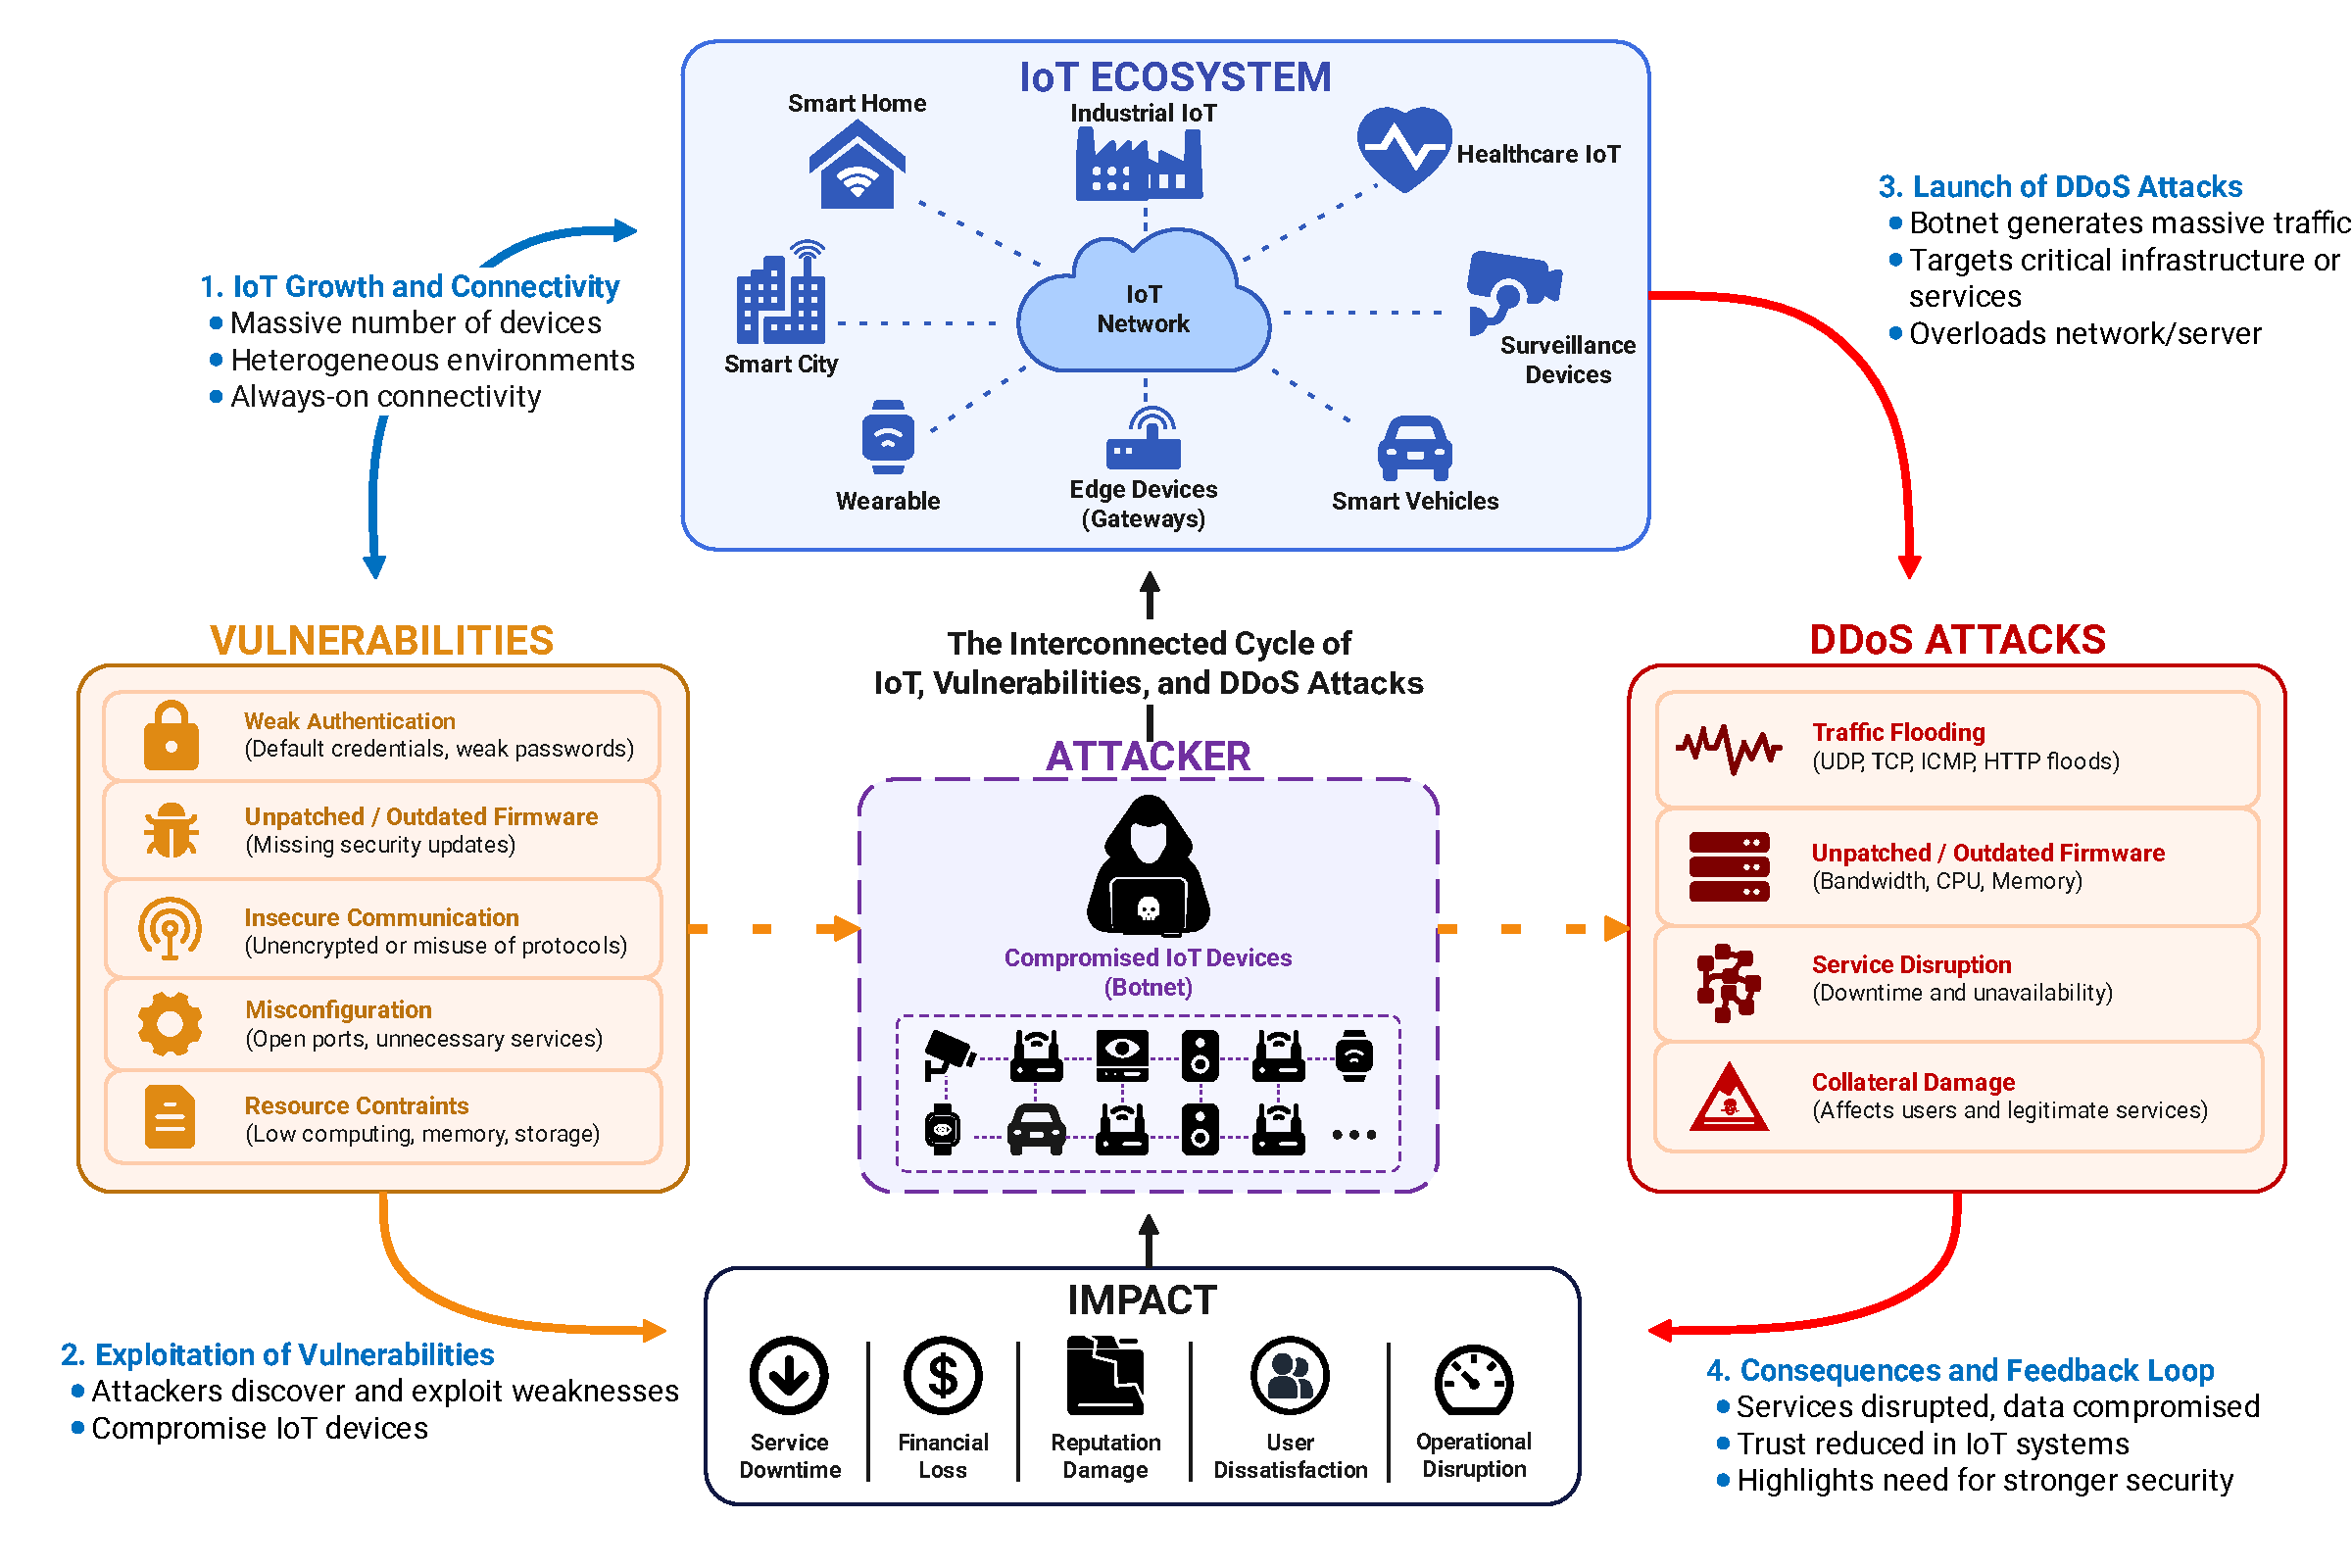
\includegraphics[width=0.98\linewidth]{figures/IoT_Ecosystem.eps}
\caption{Interconnected cycle of IoT ecosystem, vulnerabilities, and DDoS attacks.}
\label{fig:iot_ddos_cycle}
\end{figure}


To address these challenges, this study proposes a hybrid deep learning framework that integrates CNN and BiLSTM architectures with an attention-based feature gating mechanism for effective cross-dataset zero-shot IoT attack detection. Although DDoS represents a primary motivating threat class in connected environments, the proposed framework is designed to detect broad multi-vector cyber-attacks (including volumetric floods, DoS, botnets, reconnaissance, malware, MITM, web attacks, brute force, keylogging, and data exfiltration) across heterogeneous datasets. Furthermore, a multi-level XAI framework is incorporated to provide both global and local interpretability using SHAP, LIME, and ANOVA techniques. 

\subsection{Motivation}

The motivation for this work stems from several key challenges in IoT intrusion detection, including

\begin{itemize}
    \item \textbf{Heterogeneous Data Sources:} IoT datasets vary significantly in feature space, traffic patterns, and labeling schemes, making cross-dataset learning difficult.
    \item \textbf{Limited Generalization:} Existing models often perform well on a single dataset but fail when applied to unseen environments.
    \item \textbf{Limited Recurrent Feature Transformation:} Many approaches rely on purely static feature extraction and do not exploit complementary recurrent feature transformations for heterogeneous traffic representations.
    \item \textbf{Black-Box Models:} The absence of interpretability limits the adoption of deep learning-based IDS in real-world systems.
    \item \textbf{Resource Constraints in Edge/Cloud Computing Models:} Real-time deployment in modern computing models (such as edge-computing smart gateways or cloud-based IoT controllers) requires lightweight and efficient security components with minimal latency and low energy footprints.
\end{itemize}

These challenges highlight the need for a unified framework that is accurate, generalisable, interpretable, and efficient in its application.

\subsection{Proposed Approach}

To overcome the aforementioned challenges, in this study, we introduce an attention-gated hybrid CNN--BiLSTM deep learning framework for cross-dataset zero-shot IoT attack detection. The model leverages CNN layers for local spatial feature extraction and BiLSTM layers for singleton sequence bidirectional feature transformation. An attention-gating mechanism is applied to dynamically balance and rescale the spatial and recurrent representations.

In addition, a standardised dataset-specific preprocessing pipeline was employed to structure the heterogeneous network telemetry into clean feature vector representations ($T=1$), enabling robust intra- and cross-dataset evaluations. The framework is further augmented with XAI techniques to provide insights into the model’s behaviour and feature importance.

\subsection{Contributions}

The main contributions of this study are summarised as follows.

\begin{itemize}
    \item \textbf{New Design Technique for Security Components:} A novel hybrid CNN--BiLSTM+Attention framework is proposed to capture local feature interactions and learn complementary recurrent feature representations of IoT network traffic, providing an adaptable architecture for network security.

    \item \textbf{Robust Cross-Dataset Zero-Shot Transferability:} The proposed model is evaluated across multiple heterogeneous IoT datasets, demonstrating zero-shot transfer capability and protocol adaptation on unseen networks via dimensional interface adaptation.

    \item \textbf{Standardised Dataset Preprocessing and Representation Protocol:} A common preprocessing protocol with dataset-specific feature representations is established to clean, normalize, and encode heterogeneous IoT traffic features while preserving dataset-specific characteristics.

    \item \textbf{Multi-Level Explainable AI Integration:} The framework incorporates SHAP, LIME, and ANOVA to provide both global and local interpretability, ensuring that model predictions are transparent and auditable for security analysts.

    \item \textbf{Securing IoMT and Telemedicine Infrastructures:} The model is validated on medical-specific sensor network data (CIC-IoMT-2024), demonstrating its efficacy in securing safety-critical telemedicine systems against service disruption.

    \item \textbf{Deployment Feasibility and Efficiency Analysis:} The framework is evaluated in terms of GPU inference throughput and energy proxies, establishing a solid empirical foundation for future edge-device hardware validation and low-overhead security integrations.
\end{itemize}

\subsection{Organization of the Paper}

The remainder of this paper is organised as follows.  Section~\ref{sec:related} reviews the contemporary literature and state-of-the-art intrusion detection methods. Section~\ref{sec:method} details the mathematical formulation and architectural design of the proposed hybrid CNN--BiLSTM attention-gated framework. Section~\ref{sec:datasets} presents the target IoT datasets, preprocessing protocols and feature representation strategies. Section~\ref{sec:setup} outlines the experimental setup, hardware specifications, and evaluation parameters. Section~\ref{sec:results} discusses the classification performance, cross-dataset transferability, ablation studies, efficiency metrics, and multi-level XAI findings. Finally, Section~\ref{sec:conclusion} concludes the paper and highlights potential avenues for future research. 

\section{Related Work}
\label{sec:related}
This section reviews existing approaches for IoT intrusion detection, with a focus on DDoS attack detection using machine learning, deep learning, hybrid models, and explainable AI techniques.

\subsection{Machine Learning-Based Approaches}

Traditional IDSs for IoT networks have largely relied on classical machine learning techniques such as support vector machines (SVM), decision trees, random forests, and naive Bayes classifiers. These methods are effective for structured data and relatively low-dimensional feature spaces.

Several studies have applied random forest and SVM models for DDoS detection, achieving moderate accuracy on benchmark datasets. Naïve Bayes classifiers have also been explored because of their simplicity and computational efficiency. However, these approaches often suffer from limited scalability and the inability to capture complex non-linear relationships in high-dimensional IoT traffic data, as highlighted by \cite{sarhan2020evaluation}. A comparative evaluation of these machine learning configurations by \cite{verma2020machine} evaluated machine learning configurations and concluded that shallow classifiers undergo high false alarm rates under various protocols. Similarly, \cite{susilo2020security} reviewed intrusion models in smart environments and noted that random forest classifiers suffer from severe performance degradation in cross-dataset scenarios. \cite{bhamare2020machine} evaluated the feasibility of ML classifiers under software-defined network (SDN) configurations and demonstrated that SVM models are computationally expensive for real-time edge operations. To address this, \cite{AHUJA2021103108} proposed an automated DDoS attack detection framework in software-defined networking and illustrated the benefits of centralised traffic inspection for network security applications. \cite{churcher2021machine} conducted experimental evaluations on physical IoT platforms and observed that decision trees are sensitive to slight feature noise, resulting in poor generalisability. To mitigate this, \cite{soe2020machine} proposed an ensemble ML framework combining feature selection with random forest; however, their system was evaluated only on a single dataset, which leaves its generalisability unverified. \cite{habib2023multi} conducted a multi-dataset assessment of shallow ML techniques and verified that single-model classifiers fail to sustain high detection rates on unseen network configurations owing to overfitting on local feature distributions. Furthermore, \cite{indra2024ensemble} proposed an ensemble machine learning approach optimised for the imbalanced CICIDS2017 dataset to improve multiclass detection, although ensemble methods generally exhibit higher model complexity.

\subsection{Deep Learning-Based Approaches}

To overcome the limitations of classical methods, deep learning techniques have been widely adopted for IoT intrusion detection systems. CNNs have been used to extract spatial features from network traffic data, demonstrating improved performance over traditional methods.

RNNs, particularly LSTM networks, have been employed to model the temporal dependencies in sequential traffic data. These models are effective in capturing time-dependent attack patterns, which are common in DDoS attacks. Despite their advantages, standalone CNN or LSTM models often fail to fully exploit the complementary nature of spatial and temporal features. Additionally, many deep learning-based studies are limited to single dataset evaluations, raising concerns regarding their robustness for real-world deployments.

For instance, \cite{roopak2019deep} explored standalone deep learning models, including multilayer perceptrons and LSTMs, and showed that although LSTMs capture temporal trends, their spatial feature mapping is limited. \cite{latif2020lightweight} proposed a lightweight random neural network for resource-constrained IoT devices, which achieved high processing speeds but struggled to model sequential patterns. \cite{yin2020deep} utilised recurrent networks (RNNs) for NIDS and highlighted their superiority in time-series data over feed-forward networks, but noted that standard RNNs undergo vanishing gradient problems during long sequence training. \cite{basnet2022deep} applied deep neural networks to DDoS detection on the BoT-IoT dataset, achieving high accuracy but noted that deep architectures are highly sensitive to class imbalance and often ignore benign patterns. To address network traffic class imbalance, \cite{islam2026paacgan} proposed PAACGAN, a protocol-aware generative augmentation model designed to synthesise realistic minority-class attack samples and improve overall detection robustness. \cite{abbasi2021deep} developed a deep autoencoder model for anomaly detection in IoT networks, which showed high recall rates but faced challenges in real-time classification due to high latent dimensionality. For industrial Internet of Things (IIoT) systems, \cite{nguyen2022cnn} designed a CNN-based computing approach to identify botnet threats, and \cite{BENADDI2025101624} proposed a lightweight CNN to minimise edge latency, although standalone CNNs still suffer from weak temporal modelling. To address heterogeneous IIoT protocols, \cite{Jyothi2024edgeids} presented an adaptive deep learning framework for low-latency edge deployment, whereas \cite{zhou2026icsnad} worked on a real-world industrial control system dataset (ICS-NAD) to benchmark deep learning and machine learning architectures against diverse industrial control system attacks.

\subsection{Hybrid Deep Learning Models}

Recent research has explored hybrid architectures that combine multiple deep learning techniques to improve detection performance. Models that integrate CNN and LSTM layers have shown promising results by simultaneously capturing spatial and temporal patterns.

Some studies have proposed CNN-LSTM fusion models for intrusion detection, achieving higher accuracy than individual models (e.g., \citep{yan2023deep}). However, these approaches often rely on simple feature concatenation without incorporating mechanisms to dynamically prioritise important features. Furthermore, most hybrid models are evaluated using a single dataset, lacking validation across heterogeneous IoT environments. This limitation reduces their applicability in practical scenarios in which network conditions and attack patterns vary significantly.

To address these gaps, ~\cite{zhao2020hybrid} introduced a hybrid CNN-LSTM model that models spatiotemporal structures; however, their evaluation was restricted to older datasets, such as the KDD Cup 99. \cite{jiang2020network} proposed a hybrid CNN and BiLSTM model combined with an attention layer, achieving high F1-scores; however, their model suffered from a large parameter size, which increased the memory overhead of edge devices. \cite{dong2021novel} presented a hybrid model combining autoencoders with LSTMs, which showed high accuracy in botnet detection; however, they observed that feature alignment remained a major challenge. \cite{gad2021hybrid} designed a hybrid machine learning framework for intrusion detection in vehicular networks based on ToN-IoT, highlighting that although hybrid models improve detection, they fail to generalise to cross-dataset traffic. \cite{alomari2021hybrid} proposed a hybrid DL architecture for DDoS detection in smart environments, which showed improved robustness but lacked an explainability component to justify the model classifications. Other hybrid combinations have also been explored to boost spatial-temporal capability, including CNN-LSTM architectures by \cite{halbouni2022cnnlstm} and CNN-BiLSTM variations by ~ \citep{omarov2023cnnbilstm, HNAMTE2023100053}, which showed that dual branches capture localised structures and flow dynamics better. Furthermore, \cite{sadhwani2025bilstmcnn} optimised sequential mapping to reduce false alarms. To enable secure edge operations, \cite{baidar2025federated} coupled hybrid deep learning with federated learning architectures in 5G-edge ecosystems, although edge latency and communication overhead remain challenging. Recent studies have further advanced the development of hybrid deep architectures. \cite{sanyal2026litmus} designed LITMUS, a collaborative distributed host intrusion detection system (HIDS), and network intrusion detection system (NIDS) framework to mitigate dishonest collaborators, while \cite{fraihat2026hybrid} integrated a hybrid deep learning model with feature optimisation and federated learning (FL) for privacy-preserving IIoT security. To optimise client communication, \cite{khan2024federated} presented a federated reinforcement-based fusion model (Fed Inforce Fusion). Additionally, \cite{ullah2023iotids} built a CNN-GRU hybrid model for TCP flood detection, \cite{vijayan2023automated} combined a heuristic-aided autoencoder with an LSTM-based deep belief network to protect IoT-aided MQTT protocols, and \cite{poddar2024enhancing} designed a CNN-LSTM hybrid model to enhance spatiotemporal learning in cloud and edge networks. To capture temporal variations across multi-granular attack types, \cite{baig2026tide} proposed TIDE-Net, a two-stage temporal deep learning framework for IoT networks, showing that temporal architectures are highly effective at resolving complex flow sequences.

\subsection{Attention Mechanisms in IDS}

Attention mechanisms have recently been introduced to enhance deep learning models by assigning importance weights to the input features. In the context of intrusion detection, attention layers enable the model to focus on the critical features that contribute the most to attack detection.

Several studies have demonstrated that attention-based models improve classification performance and interpretability. However, the integration of attention mechanisms with hybrid CNN-LSTM architectures for IoT DDoS detection remains relatively underexplored, particularly in multi-dataset settings. \cite{hosseini2024attention} applied self-attention mechanisms to NIDS and demonstrated that attention layers can focus on key traffic indicators; however, their system was not optimised for low-latency IoT networks. \cite{zhou2021ddos} integrated an attention layer with LSTMs to detect DDoS attacks, showing improved convergence; however, their architecture ignored spatial feature correlations. \cite{gu2022lightweight} designed an attention-based CNN-GRU model to achieve high throughput but did not validate the framework against adversarial perturbations or modern multi-protocol datasets. Swain et al.~\cite{wu2023lightweight} proposed a lightweight hybrid model with self-attention for edge networks, which reduced latency but achieved suboptimal performance on highly imbalanced multiclass datasets. To address these gaps, \cite{dai2024cnnbilstmattention} and \cite{naeem2025attentioncnnbilstm} combined CNN and BiLSTM with self-attention to prioritise critical features, thereby improving the overall detection accuracy. Similarly, \cite{alashjaee2025deep} and \cite{purbia2026iaids} proposed intelligent adaptive systems that utilised attention weighting to improve multiclass separation under high traffic volumes. For complex sequences, \cite{zhang2025cnnbilstmtransformer} leveraged transformer-based attention alongside CNN-BiLSTM to capture the long-range temporal context, although at the expense of a higher resource complexity. Furthermore, \cite{elwhishi2026ckan} proposed an attention-enhanced hybrid CKAN-BiLSTM architecture for efficient intrusion detection; \cite{priyadarshini2023attention} integrated an attention-based BiLSTM-CNN for software-defined network (SDN) and application-layer DDoS detection; and \cite{zhang2023transformer} used a transformer-based IDS to capture long-range dependencies, showing high accuracy but requiring substantial computational resources that are unsuitable for edge deployment.

\subsection{Explainable AI in Intrusion Detection}

XAI has gained increasing attention in cybersecurity applications, where model transparency is essential. Techniques such as SHapley Additive exPlanations (SHAP)~\citep{lundberg2017unified} and Local Interpretable Model-agnostic Explanations (LIME)~\citep{ribeiro2016why} have been used to interpret the model predictions.

Although these methods provide valuable insights into feature importance and decision-making processes, their adoption in IoT intrusion detection systems remains limited. Most existing studies focus primarily on improving accuracy, with little emphasis on interpretability and trustworthiness, as discussed by \cite{hnamte2024iot}. Additionally, few studies have combined multiple XAI techniques with statistical validation methods, such as ANOVA, to provide comprehensive explanation frameworks.

\cite{almimi2023xai} surveyed explainable artificial intelligence techniques in intrusion detection and noted that local interpretable surrogates are crucial for threat verification. \cite{shaaban2023biomt} developed an explainable IDS for the IoMT using SHAP to highlight critical features; however, their model did not incorporate temporal relationships. \cite{liu2022explainable} conducted a survey on XAI for IoT security and stated that explainability must be integrated with robust cross-dataset learning to ensure that model decisions remain stable across different network topologies. To address model interpretability, \cite{singh2023xai} established an explainable AI framework utilising SHAP and LIME to interpret deep learning decisions locally and globally. Additionally, \cite{gupta2026novaxids} proposed NOVA-XIDS, an explainable latent-attention hybrid deep learning framework for high-fidelity intrusion detection in IoT and industrial cyber systems, combining autoencoder latent spaces with SHAP and CBAM visual attention to achieve both generalisation and transparency.

\subsection{Research Gaps}

The following key limitations were identified based on the above review.

\begin{itemize}
    \item \textbf{Limited Generalization:} Most existing approaches are evaluated on single datasets, limiting their applicability to diverse IoT environments.
    
    \item \textbf{Inadequate Feature Integration:} Traditional and deep learning models often fail to effectively combine spatial feature maps and channel-wise recurrent representations.
    
    \item \textbf{Lack of Adaptive Feature Weighting:} Many hybrid models do not incorporate attention mechanisms to dynamically prioritize important features.
    
    \item \textbf{Absence of Explainability:} Existing intrusion detection systems largely operate as black boxes, lacking interpretability.
    
    \item \textbf{Insufficient Evaluation:} Few studies perform comprehensive evaluations including cross-dataset testing and efficiency assessment.
\end{itemize}

Additionally, as discussed by \cite{sgouras2022detecting}, current IoT intrusion frameworks fail to handle the feature heterogeneity introduced by multi-protocol smart grids. \cite{kumar2021eddos} proposed a distributed intrusion detection framework for blockchain-enabled fog environments, which achieved high detection rates but incurred significant resource overheads, highlighting the need for efficient edge-oriented models.

\subsection{Positioning of the Proposed Work}

To address these limitations, this study proposes a hybrid CNN--BiLSTM+Attention framework that integrates spatial convolution and recurrent feature transformation with attention-based feature weighting. Unlike existing approaches, the proposed model was evaluated across multiple heterogeneous IoT datasets (Apose-IoT-23~\citep{pecorella2021iot}, BoT-IoT~\citep{moustafa2015bot}, CIC-IoMT-2024~\citep{iomt2024dataset}, and CIC-IoT-2025~\citep{ciciot2025dataset}), ensuring robust generalisation. Furthermore, the integration of SHAP, LIME, and analysis of variance (ANOVA) provides a comprehensive explainability framework that enhances the transparency and trust in the model predictions. The proposed approach also includes an extensive evaluation through efficiency analysis, making it suitable for real-world IoT deployments. A comprehensive comparison of the proposed model with existing related works is summarised in Table~\ref{tab:related_works_comparison}.

{\small
\begin{landscape}
\begin{longtable}{p{4cm}p{4cm}p{4cm}p{4cm}p{4cm}}
\caption{Comparison of related works in IoT intrusion and DDoS detection}
\label{tab:related_works_comparison}\\
\hline
Study &
  Proposed Method &
  Key Findings &
  Limitations &
  Research Gaps \\ \hline
\endfirsthead
%
\multicolumn{5}{c}%
{{\bfseries Table \thetable\ continued from previous page}} \\
\hline
Study &
  Proposed Method &
  Key Findings &
  Limitations &
  Research Gaps \\ \hline
\endhead
%
\hline
\endfoot
%
\endlastfoot
%
\cite{verma2020machine} &
  Machine learning evaluation &
  Compares classifiers on IoT benchmarks &
  Single-node evaluation &
  Lacks multi-dataset deep learning benchmarks \\
\cite{roopak2019deep} &
  CNN + LSTM hybrid DL &
  High accuracy on DDoS subclass &
  Tested only on CICIDS2017 &
  No cross-dataset analysis or explainability \\
\cite{kumar2021eddos} &
  Deep Learning DDoS framework &
  Improved recall on IoT traffic &
  Heavy model architecture &
  High latency, unsuitable for real-time edge \\
\cite{latif2020lightweight} &
  Lightweight Random Neural Network &
  Low prediction latency &
  Evaluated on older feature sets &
  Lacks deep spatial-temporal feature mapping \\
\cite{zhao2020hybrid} &
  CNN-LSTM model &
  Captured spatial-temporal structures &
  Evaluated on older datasets &
  No validation on modern IoT/IoMT environments \\
\cite{jiang2020network} &
  CNN-BiLSTM + Attention &
  Dynamic weight assignment &
  Complex, high parameter size &
  Missing inference latency/energy proxy checks \\
\cite{zhou2021ddos} &
  Attention-LSTM model &
  High F1-score for DDoS classification &
  Captures only temporal structures &
  Ignores spatial/feature-level correlations \\
\cite{wu2023lightweight} &
  Edge hybrid model &
  Balanced speed and accuracy &
  Restricted to single dataset &
  Gaps in explainability and model trust \\
\cite{gu2022lightweight} &
  Attention-CNN-GRU &
  High throughput for benign/attack &
  Lacks robustness under class imbalance &
  Lacks global SHAP/local LIME validation \\
\cite{basnet2022deep} &
  Deep learning DDoS detection &
  Effective multiclass separation &
  Lacks standardised feature preprocessing &
  Cannot generalize to unseen IoT protocols \\
\cite{almimi2023xai} &
  XAI framework survey &
  Highlighted importance of model trust &
  Review only, no implementation &
  Lacks integration with hybrid DL models \\
\cite{sarhan2020evaluation} &
  Feature set evaluation (NetFlow vs CIC) &
  NetFlow features improve generalizability and NIDS adaptiveness &
  Lacks integration of deep sequential architectures &
  Does not analyze cross-dataset performance with temporal models \\
\cite{yan2023deep} &
  CNN+LSTM hybrid NIDS &
  Captures spatial-temporal IIoT traffic features with 99.84\% accuracy &
  No attention weighting or bidirectional temporal modelling &
  Lacks cross-dataset validation and model explainability \\
\cite{hnamte2024iot} &
  Deep neural network DDoS detection &
  High accuracy (99.99\%) with XAI validation of predictions &
  Evaluated primarily under static SDN network topologies &
  Gaps in generalizing across highly heterogeneous IoT networks \\
\cite{sgouras2022detecting} &
  ML DDoS impact analysis in smart grids &
  Quantified cyberattack impact on smart grid infrastructure stability &
  Heavy focus on impact metrics rather than real-time NIDS &
  Lacks modern multi-protocol feature validation \\
\cite{hosseini2024attention} &
  IoT-PRIDS (Packet representation) &
  Leverages packet representation learning for robust NIDS &
  High feature extraction latency, unsuited for edge deployment &
  Gaps in global model explainability under class imbalance \\
\cite{susilo2020security} &
  Deep learning algorithm NIDS in IoT &
  Explores MLP and LSTM structures for cyber anomaly detection &
  Severe performance degradation under cross-dataset traffic &
  Missing statistical feature selection (like ANOVA) and local XAI \\
\cite{yin2020deep} &
  RNN-based NIDS &
  RNNs outperform feed-forward networks in modelling sequential traffic &
  Vanishing gradients during long sequence learning; high latency &
  Lacks spatial feature extraction and attention weight tuning \\
\cite{shaaban2023biomt} &
  Explainable IDS for IoMT &
  High performance on healthcare devices with local SHAP interpretability &
  Evaluated on static features; ignores temporal relationships &
  Lacks bidirectional sequence modelling \\
\cite{dong2021novel} &
  Autoencoder-LSTM hybrid &
  Two-stage model improves botnet detection accuracy via autoencoders &
  Spatial feature-level correlations are ignored; high training overhead &
  No validation on cross-dataset configurations or explainability \\
\cite{liu2022explainable} &
  Explainable NIDS survey &
  Highlights opportunities for SHAP/LIME in NIDS transparency &
  Survey paper, lacks experimental hybrid DL model evaluation &
  Does not propose a unified framework for cross-dataset trust \\
\cite{bhamare2020machine} &
  Supervised ML for cloud security &
  SVMs and Decision Trees achieve good anomaly classification rates &
  SVM is too computationally expensive for real-time edge nodes &
  Lacks deep sequential modelling and multi-dataset benchmarks \\
\cite{churcher2021machine} &
  Experimental evaluation of ML NIDS &
  Analyzed classifier sensitivity to feature noise and hardware constraints &
  Decision trees display low generalizability under traffic fluctuations &
  No deep learning or spatial-temporal feature fusion explored \\
\cite{soe2020machine} &
  Ensemble ML with feature selection &
  Wrapper feature selection improves RF accuracy to 99\% &
  Evaluated on single dataset; sensitive to protocol drift &
  Lacks explainability and deep temporal learning \\
\cite{abbasi2021deep} &
  Memory-augmented autoencoder NIDS &
  Effectively models normal patterns to identify anomalies &
  High computational latency due to memory networks; unsuited for edge &
  No sequence modelling (like BiLSTM) or global explanations \\
\cite{alomari2021hybrid} &
  Parallel hybrid DL DDoS detection &
  Parallel architectures capture features faster and with higher accuracy &
  Lacks standardised preprocessing, leading to poor generalization &
  Gaps in transparency; no local or global XAI models \\
\cite{habib2023multi} &
  Multi-dataset standardization &
  Standardizing NetFlow features improves cross-dataset NIDS stability &
  Tested only on shallow classifiers; lacks deep sequence extraction &
  Gaps in attention refinement and deep learning integration \\
\cite{sanyal2026litmus} &
  Hybrid distributed HIDS+NIDS (LITMUS) &
  Robust mimicry attack detection with collaborative IDS &
  Focus on HMA only &
  Limited DL-based feature learning and XAI integration \\
\cite{fraihat2026hybrid} &
  HGS-CS + Transformer-LSTM + FL &
  High accuracy (99\%) with privacy-preserving learning &
  High computational complexity &
  Lacks lightweight edge deployment validation \\
\cite{zhou2026icsnad} &
  ICS-NAD dataset + ML/DL benchmarking &
  Real-world ICS dataset with 20 attack types &
  Dataset-only contribution &
  Lack of integrated detection framework \\
\cite{elwhishi2026ckan} &
  CKAN-BiLSTM + Attention &
  Lightweight and interpretable IDS with strong performance &
  Single dataset validation &
  Limited cross-dataset generalisation \\
\cite{khan2024federated} &
  Federated IDS with RL fusion &
  Privacy-preserving collaborative detection &
  High communication overhead &
  Limited explainability \\
\cite{ullah2023iotids} &
  CNN-GRU hybrid model &
  Effective temporal feature extraction &
  Dataset-specific tuning &
  No XAI validation \\
\cite{vijayan2023automated} &
  Deep autoencoder + LSTM &
  Improved anomaly detection accuracy &
  High training time &
  Poor real-time feasibility \\
\cite{priyadarshini2023attention} &
  Attention-based BiLSTM IDS &
  Enhanced feature weighting &
  Ignores spatial correlations &
  No multi-dataset evaluation \\
\cite{nguyen2022cnn} &
  CNN-based IDS &
  Fast feature extraction &
  Weak temporal modelling &
  Limited adaptability \\
\cite{indra2024ensemble} &
  Ensemble ML for IoT IDS &
  Robust classification under imbalance &
  High model complexity &
  No deep feature learning \\
\cite{Jyothi2024edgeids} &
  Edge-based lightweight IDS &
  Low latency detection &
  Reduced accuracy &
  Limited scalability \\
\cite{zhang2023transformer} &
  Transformer-based IDS &
  Captures long-range dependencies &
  High computational cost &
  Not suitable for edge deployment \\
\cite{poddar2024enhancing} &
  CNN-LSTM hybrid IDS &
  Balanced spatial-temporal learning &
  Requires hyperparameter tuning &
  Lacks explainability \\
\cite{singh2023xai} &
  XAI-based IDS (SHAP/LIME) &
  Improved model interpretability &
  No hybrid DL integration &
  Limited performance benchmarking \\
\cite{BENADDI2025101624} &
  Lightweight CNN IDS &
  Efficient for IoT devices &
  Reduced detection accuracy &
  Poor handling of complex attacks \\
\cite{gupta2026novaxids} &
  Explainable Latent-Attention NIDS (NOVA-XIDS) &
  High-fidelity detection with global latent space embeddings &
  High computational latency &
  Lacks dynamic edge streaming verification \\
\cite{islam2026paacgan} &
  PAACGAN (Protocol-Aware GAN) &
  Augments minority attack traffic realistically &
  Requires GAN adversarial training &
  Not validated on cross-dataset transfers \\
\cite{baig2026tide} &
  Two-stage temporal TIDE-Net (BiLSTM) &
  Handles temporal flow sequence classification &
  Higher computational overhead &
  No spatial feature extraction branch \\
\textbf{Proposed Work} &
  Hybrid CNN--BiLSTM+Attention &
  Spatial-recurrent fusion with XAI &
  Validated offline on traces &
  Physical deployment on live edge nodes \\ \hline
\end{longtable}
\end{landscape}
}

\section{Methodology}
\label{sec:method}
This section presents the proposed hybrid deep learning framework for IoT attack detection. The overall architecture of the system is illustrated in Figure~\ref{fig:proposed_pipeline}, which depicts the complete pipeline from data acquisition to explainability.

\begin{landscape}
\begin{figure*}
\centering
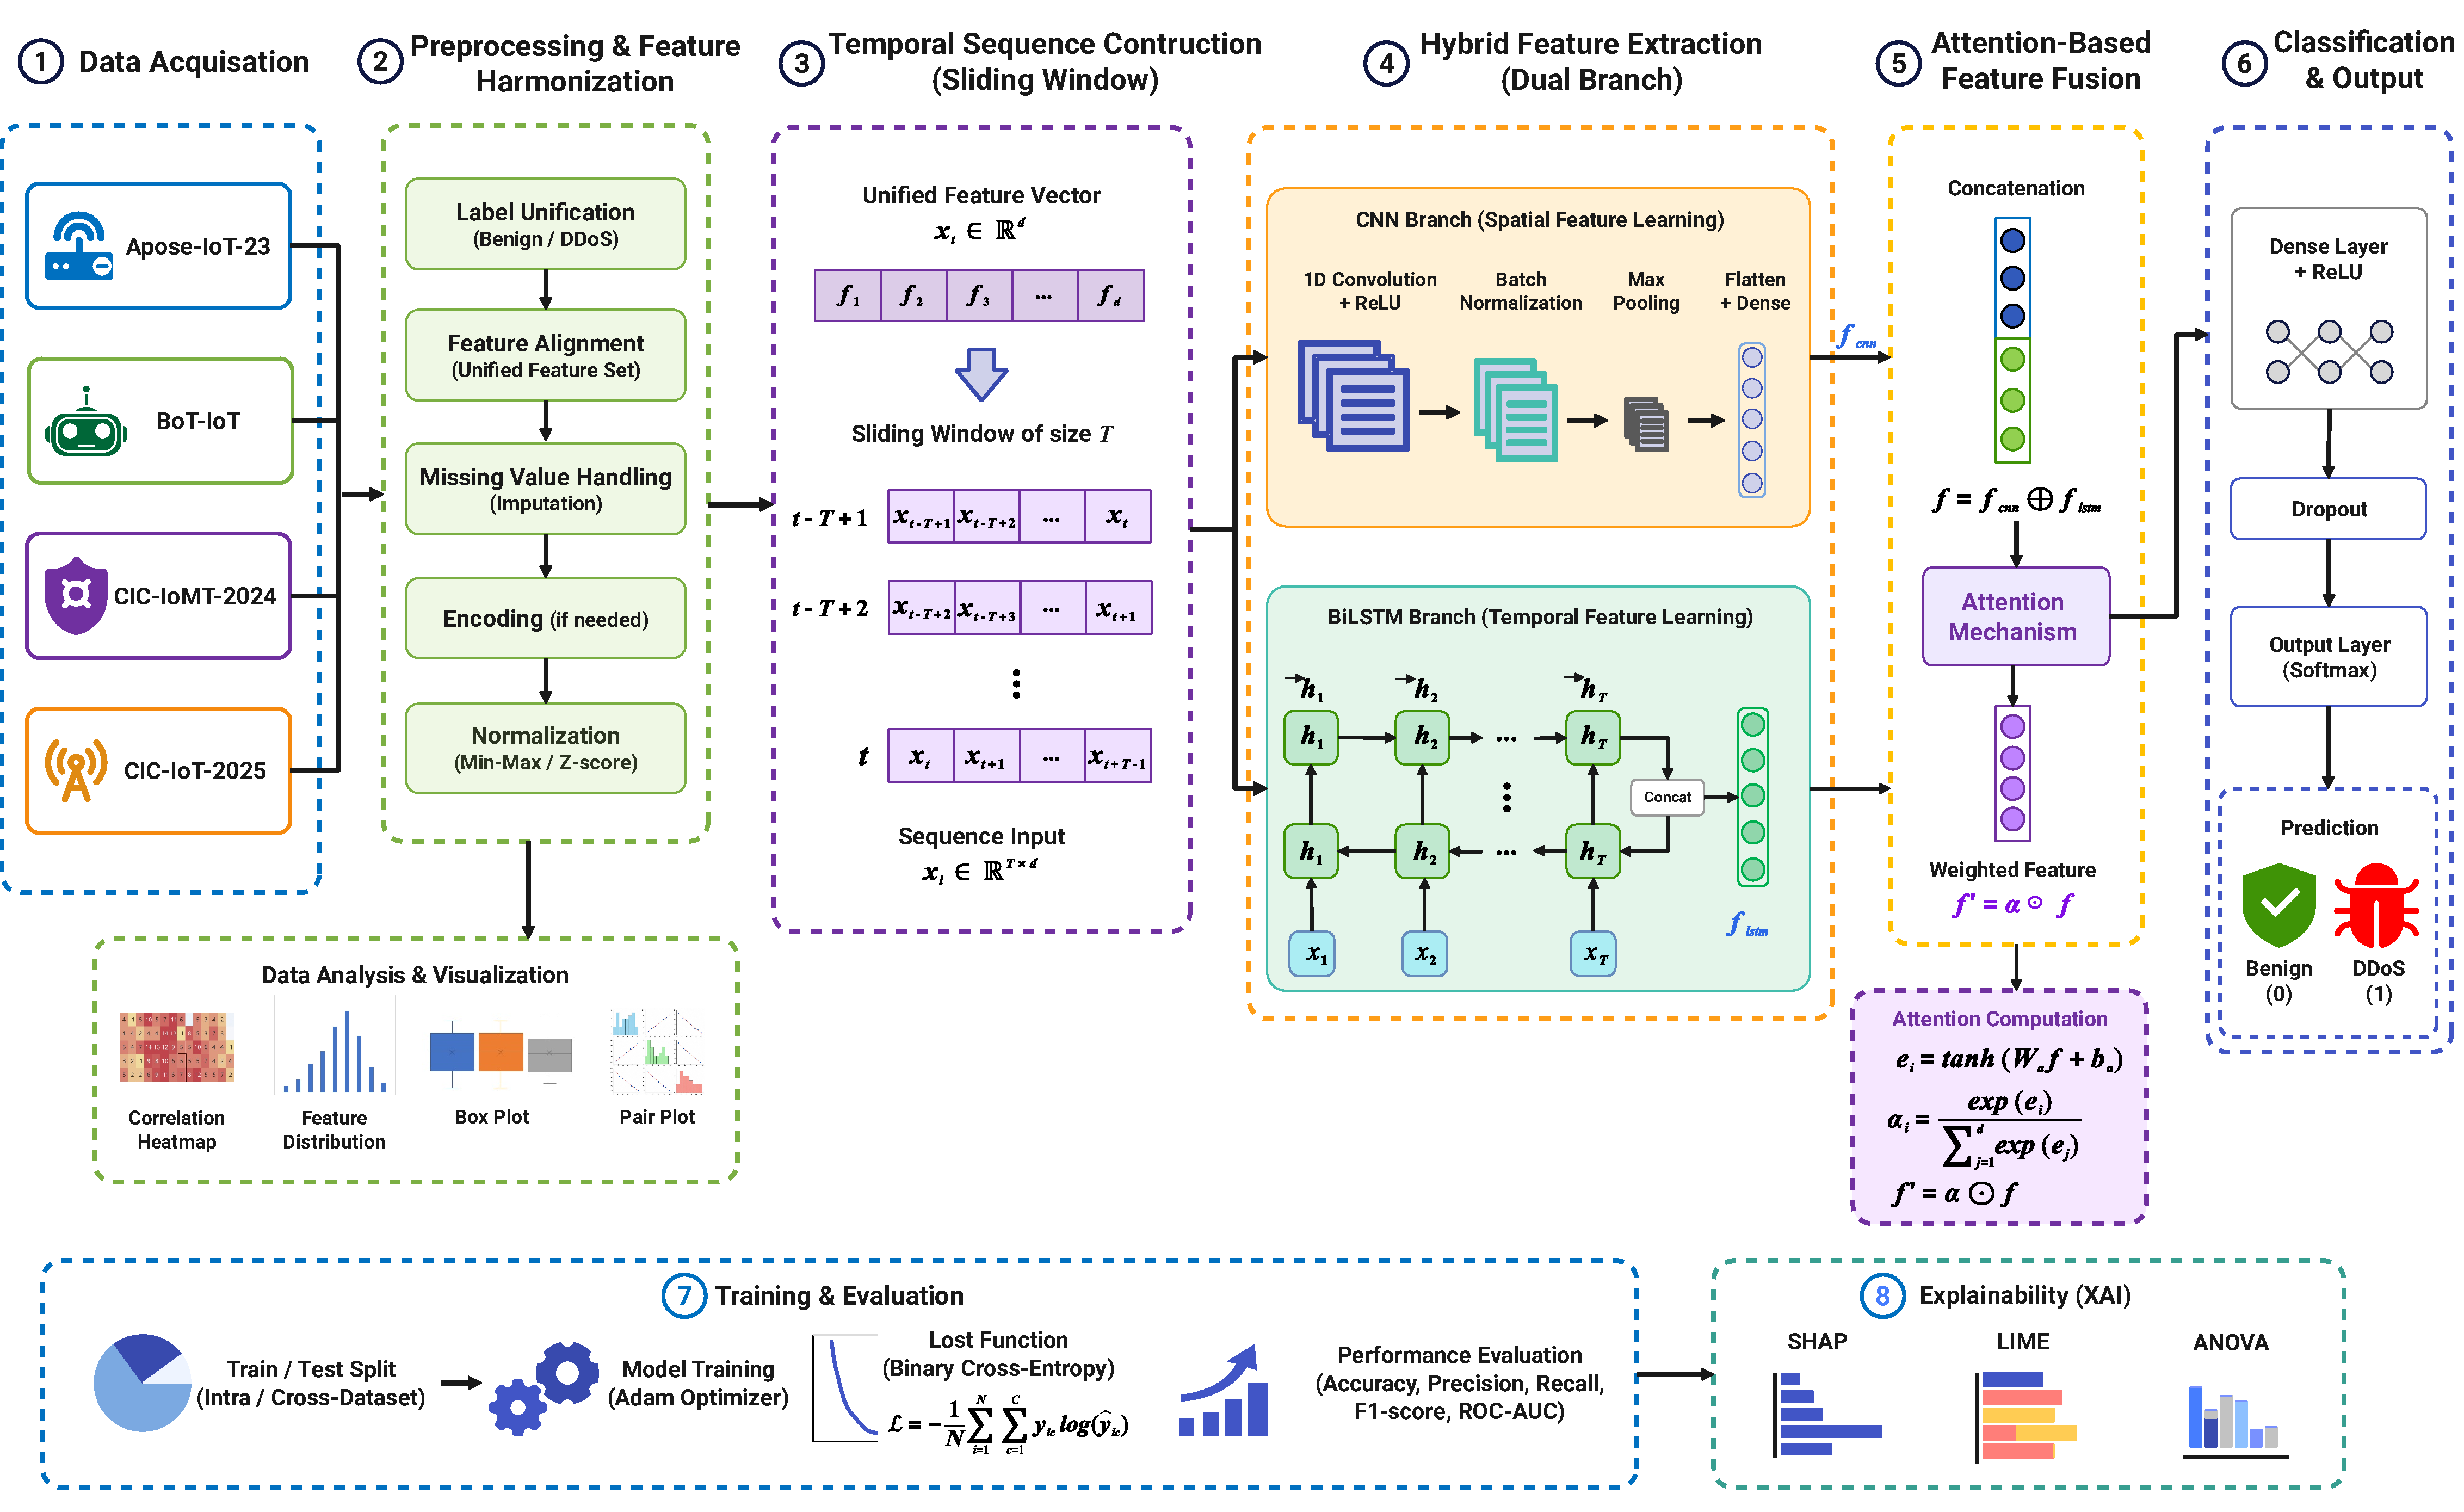
\includegraphics[width=0.98\linewidth]{figures/Model_Pipeline_Architecture.pdf}
\caption{Proposed hybrid CNN--BiLSTM + Attention framework for IoT attack detection}
\label{fig:proposed_pipeline}
\end{figure*}
\end{landscape}


As shown in Figure~\ref{fig:proposed_pipeline}, the proposed framework consists of multiple sequential stages: data acquisition, dataset-specific feature preprocessing, temporal sequence construction, parallel convolutional and recurrent feature extraction (via CNN and BiLSTM branches), attention-based feature refinement, classification, and multi-level explainability. Each component is mathematically formulated and integrated to address the challenges of heterogeneous, high-velocity IoT network flows.

\subsection{Problem Definition}

Let $\mathcal{D}^{(k)} = \{(x_i^{(k)}, y_i^{(k)})\}_{i=1}^{N_k}$ denote the $k$-th IoT dataset under analysis, where $N_k$ represents the number of flow samples. Here, $x_i^{(k)} \in \mathbb{R}^{d_k}$ is the raw feature vector representing network packet headers and flow statistics in a dataset-specific $d_k$-dimensional feature space, and $y_i^{(k)}$ is the target label, respectively. For binary threat detection, the labels belong to the space $y_i^{(k)} \in \mathcal{Y}_{bin} = \{0, 1\}$, where $0$ represents benign traffic and $1$ represents malicious or attack traffic. For multiclass intrusion categorisation, the labels belong to the space $y_i^{(k)} \in \mathcal{Y}_{multi} = \{0, 1, \dots, C-1\}$, where $C$ is the number of distinct traffic subclasses (benign traffic plus specific threat vectors such as HTTP flood, UDP flood, TCP SYN flood, malware, and reconnaissance).

Given $K$ heterogeneous IoT datasets with different feature dimensions ($d_1 \neq d_2 \neq \dots \neq d_K$) and class schemas, our goal is to design a standardised preprocessing operator $\phi_k(\cdot)$ and learn a robust, generalisable classifier $f_\theta: \mathbb{R}^{d_k} \rightarrow \mathcal{Y}$ parameterised by weights $\theta$ that minimises detection error across both intra-dataset and cross-dataset evaluation setups.

\subsection{Dataset-Specific Feature Preprocessing and Representation}

To handle the heterogeneous feature spaces produced by different network telemetry collectors, the final retained feature dimensionalities were $d_k = 16, 28, 45,$ and $84$ for Apose-IoT-23, BoT-IoT, CIC-IoMT-2024, and CIC-IoT-2025, respectively. Each dataset $k$ is preprocessed according to its dataset-specific feature space $\mathcal{F}^{(k)} \subset \mathbb{R}^{d_k}$. (The feature-subset ablation in Section~\ref{sec:feature_ablation} separately evaluates reduced subsets of 5, 12, 20, and 20 features, respectively.) Rather than forcing a lossy intersection across datasets during individual model training, a standardised preprocessing operator $\phi_k(\cdot)$ is defined to map each raw feature vector $x_i^{(k)} \in \mathbb{R}^{d_k}$ into a clean and structured representation as follows:

\begin{equation}
x_i'^{(k)} = \phi_k(x_i^{(k)}) \in \mathbb{R}^{d_k}
\end{equation}

The dataset-specific preprocessing operator $\phi_k(\cdot)$ executes three core operations:
\begin{enumerate}
    \item \textbf{Feature Alignment and Imputation:} Cleaning raw packet headers and flow statistics, handling missing or infinite values via localized mean imputation.
    \item \textbf{Categorical Encoding:} Converting nominal protocol and service identifiers (e.g., TCP, UDP, ICMP, HTTP) into numerical representations using ordinal label factorization. Categorical encoders were fitted exclusively on the training partition ($D_{train}$), and the resulting category-to-integer mappings were applied unchanged to the validation and test partitions. Subsequent 1D-CNN spatial filtering and BiLSTM feature-channel embedding learn continuous non-linear representations from these encoded feature channels.
    \item \textbf{Statistical Z-Score Normalization:} Standardizing feature magnitudes to prevent large-scale attributes from dominating gradient updates.
\end{enumerate}

Crucially, all feature selection and ranking operations (including ANOVA F-statistic rankings and XAI importance scoring) were performed exclusively on the training partition ($D_{train}$); the selected feature subsets were then fixed prior to validation and test evaluation, ensuring that all feature-ablation experiments remained strictly leak-free.

To ensure numerical stability during gradient backpropagation and prevent features with larger scales from dominating the loss, Z-score normalisation was applied to each feature dimension:

\begin{equation}
\mathbf{x}_i = \frac{x_i'^{(k)} - \mu^{(k)}}{\sigma^{(k)}}
\end{equation}

where $\mu^{(k)} \in \mathbb{R}^{d_k}$ and $\sigma^{(k)} \in \mathbb{R}^{d_k}$ are the mean and standard deviation vectors computed over the training split of dataset $k$, respectively.

\subsection{Zero-Shot Cross-Dataset Feature Dimensional Adaptation}

When performing zero-shot cross-dataset evaluation across heterogeneous IoT environments, a model parameterised by weights $\theta$ trained on source dataset $A$ (with input feature space dimension $d_{\text{src}}$) must evaluate target dataset $B$ (with feature space dimension $d_{\text{tgt}}$). To enable direct zero-shot inference without retraining or modifying the input layer dimensions of the trained source model checkpoint, a deterministic dimensional adaptation mapping operator $\psi_{\text{src} \leftarrow \text{tgt}}: \mathbb{R}^{d_{\text{tgt}}} \rightarrow \mathbb{R}^{d_{\text{src}}}$ is defined as follows:

\begin{equation}
\psi_{\text{src} \leftarrow \text{tgt}}(\mathbf{x}) = 
\begin{cases}
\mathbf{x}, & \text{if } d_{\text{tgt}} = d_{\text{src}} \\[1.5ex]
\left[ \mathbf{x} \,\|\, \mathbf{0}_{d_{\text{src}} - d_{\text{tgt}}} \right], & \text{if } d_{\text{tgt}} < d_{\text{src}} \quad \text{(Zero-Padding Adaptation)} \\[1.5ex]
\mathbf{x}_{1:d_{\text{src}}}, & \text{if } d_{\text{tgt}} > d_{\text{src}} \quad \text{(Feature Truncation Adaptation)}
\end{cases}
\label{eq:cross_dataset_alignment}
\end{equation}

where $\mathbf{x} \in \mathbb{R}^{d_{\text{tgt}}}$ is the target feature vector standardised via Z-score normalization $\mathbf{x} = (\mathbf{x}_{\text{raw}} - \mu_{\text{tgt}}) / \sigma_{\text{tgt}}$. Here, the normalisation parameters $\mu_{\text{tgt}} \in \mathbb{R}^{d_{\text{tgt}}}$ and $\sigma_{\text{tgt}} \in \mathbb{R}^{d_{\text{tgt}}}$ are calculated strictly from the training split of the target dataset ($D_{\text{train}}^{(\text{tgt})}$), representing an unsupervised target domain normalisation setup. For cross-dataset transfer, categorical encoding mappings and numerical preprocessing parameters were obtained independently from the target training partition and applied unchanged to the target validation/test data before the dimensional adaptation operator was applied. Crucially, no statistics or label information are computed from the target test partition ($D_{\text{test}}^{(\text{tgt})}$), guaranteeing no data leakage from the test set. The operator $[\mathbf{a} \,\|\, \mathbf{b}]$ denotes vector concatenation, $\mathbf{0}_{k} \in \mathbb{R}^k$ represents a zero-padding vector of dimension $k = d_{\text{src}} - d_{\text{tgt}}$, and $\mathbf{x}_{1:d_{\text{src}}} = [x_1, x_2, \dots, x_{d_{\text{src}}}]^T$ selects the leading $d_{\text{src}}$ attribute channels. This operator performs positional dimensional adaptation to conform target feature vectors to the input dimensionality of the source model checkpoint ($d_{\text{src}}$) without modifying trained weight matrices. Because attribute ordering is determined by each collector's native feature layout rather than semantic feature matching, this operator provides a lightweight dimensional interface rather than a guaranteed semantic feature harmonisation.

\subsection{Sequence Framing and Partitioning Hygiene}

To process the flow feature representations within the hybrid architecture, normalised feature vectors $\mathbf{x}_i \in \mathbb{R}^{d_k}$ are structured into a sequence matrix $\mathbf{X}_i \in \mathbb{R}^{T \times d_k}$. In temporal sliding window approaches where lookback window length $T > 1$, consecutive sequence windows share $T-1$ overlapping flow records. Applying a random flow-level split on overlapping sliding windows ($T > 1$) introduces temporal data leakage between training, validation, and testing partitions.
To guarantee complete independence among experimental splits and prevent synthetic metrics driven by data leakage, we enforced a strict singleton sequence framing ($T = 1$):

\begin{equation}
\mathbf{X}_i = [\mathbf{x}_i]^T \in \mathbb{R}^{1 \times d_k}
\end{equation}

With $T = 1$, each network flow sample was processed as an independent-feature sequence. Consequently, the BiLSTM branch operates on singleton sequences ($T = 1$) and performs a singleton-sequence bidirectional feature transformation, refining non-linear feature representations without assuming multi-flow temporal dependencies or introducing overlapping window leakage across data partitions.

\subsection{Architectural Components of the Proposed Framework}

The proposed framework employs a dual-branch parallel architecture consisting of a 1D convolutional neural network (1D-CNN) branch for spatial feature extraction, a bidirectional long short-term memory (BiLSTM) branch for singleton-sequence bidirectional feature transformation, and a dynamic softmax attention-based feature gating layer.

\subsubsection{1D-CNN Branch (Spatial Feature Extraction)}

The 1D-CNN branch extracts local spatial dependencies and interfeature correlations from the structured input tensor $\mathbf{X}_i \in \mathbb{R}^{1 \times d_k}$.

For the 1D convolutional layer, feature representations are generated by sliding kernels across the feature vector dimensions as follows:

\begin{equation}
z_{cnn, i} = \sigma(W_c * \mathbf{X}_i + b_c)
\end{equation}

where $*$ denotes the 1D convolution operator, $W_c$ represents the convolution filter weights, $b_c$ is the bias term, and $\sigma(\cdot)$ represents the rectified linear unit (ReLU) activation function.

To downsample the spatial representation and retain only the most prominent feature excitations, max-pooling is applied, and the resulting pooled feature maps are flattened to yield the spatial representation vector $f_{cnn}$:

\begin{equation}
f_{cnn} = \text{Flatten}(p_{cnn}) \in \mathbb{R}^{D_{cnn}}
\end{equation}

\subsubsection{BiLSTM Branch (Singleton-Sequence Bidirectional Feature Transformation)}

Whereas the 1D-CNN branch extracts local spatial feature interactions, the BiLSTM branch performs a single-sequence bidirectional feature transformation. For $T=1$, the bidirectional LSTM cell processes the single-flow feature vector through forward and backward recurrent states, learning complementary feature representations without assuming multi-flow temporal sequences or risking cross-split-window leakage.

For the input sequence $\mathbf{X}_i = [\mathbf{x}_1]^T \in \mathbb{R}^{1 \times d_k}$, a forward LSTM cell processes the single-step input, updating its hidden state $\overrightarrow{h}_t \in \mathbb{R}^{d_{lstm}}$ and cell state $c_t \in \mathbb{R}^{d_{lstm}}$ through the following gating mechanisms:

\begin{align}
i_t &= \sigma_{sig} \left( W_{xi} \mathbf{x}_t + W_{hi} \overrightarrow{h}_{t-1} + b_i \right) \\
f_t &= \sigma_{sig} \left( W_{xf} \mathbf{x}_t + W_{hf} \overrightarrow{h}_{t-1} + b_f \right) \\
o_t &= \sigma_{sig} \left( W_{xo} \mathbf{x}_t + W_{ho} \overrightarrow{h}_{t-1} + b_o \right) \\
\tilde{c}_t &= \tanh \left( W_{xc} \mathbf{x}_t + W_{hc} \overrightarrow{h}_{t-1} + b_c \right) \\
c_t &= f_t \odot c_{t-1} + i_t \odot \tilde{c}_t \\
\overrightarrow{h}_t &= o_t \odot \tanh(c_t)
\end{align}

where $i_t$, $f_t$, and $o_t$ represent the input, forget, and output gates, respectively; $\tilde{c}_t$ is the candidate cell state; $\sigma_{sig}(z) = (1 + e^{-z})^{-1}$ is the sigmoid activation; and $\odot$ denotes element-wise vector multiplication.

Concurrently, a backward LSTM cell processes the single-step input in reverse feature ordering to capture complementary channel-wise feature context.

\begin{equation}
\overleftarrow{h}_t = \text{LSTM}_{back}(\mathbf{x}_t, \overleftarrow{h}_{t+1})
\end{equation}

The final recurrent representation $f_{lstm}$ is constructed by concatenating the hidden states of both directional sweeps ($T=1$) as follows:

\begin{equation}
f_{lstm} = [\overrightarrow{h}_1 \oplus \overleftarrow{h}_1] \in \mathbb{R}^{2 d_{lstm}}
\end{equation}

\subsection{Feature Fusion}

The spatial feature vector $f_{cnn}$ and the recurrent feature vector $f_{lstm}$ are concatenated to create the joint representation vector $f$:

\begin{equation}
f = [f_{cnn} \oplus f_{lstm}] \in \mathbb{R}^{D_{fused}}
\end{equation}

where $D_{fused} = D_{cnn} + 2 d_{lstm}$.

\subsection{Attention-Based Feature Refinement}

To prevent the model from being overloaded by noisy or redundant spatial and recurrent features, an attention-based feature-gating mechanism is applied. This layer assigns dynamic weights to the components of the fused feature vector $f$, emphasising critical feature correlations.

First, the fused vector is passed through a dense layer to project it into an attention energy space.

\begin{equation}
e = \tanh(W_a f + b_a)
\end{equation}

where $W_a \in \mathbb{R}^{D_{fused} \times D_{fused}}$ is the attention weight matrix and $b_a \in \mathbb{R}^{D_{fused}}$ is the attention bias vector.

The attention weights $\alpha \in \mathbb{R}^{D_{fused}}$ are computed using a softmax activation function:

\begin{equation}
\alpha_i = \frac{\exp(e_i)}{\sum_{j=1}^{D_{fused}} \exp(e_j)}
\end{equation}

The refined feature representation $\tilde{f}$ is obtained by performing element-wise multiplication between the attention weight vector $\alpha$ and the fused feature vector $f$:

\begin{equation}
\tilde{f} = \alpha \odot f \in \mathbb{R}^{D_{fused}}
\end{equation}

This dynamic weighting suppresses noisy, non-contributing dimensions and highlights relevant spatial and recurrent feature correlations..

\subsection{Classification Layer}

The refined representation $f'$ is mapped to the target output space using a fully connected layer as follows:

\begin{equation}
z = W_o f' + b_o
\end{equation}

where $W_o \in \mathbb{R}^{C \times D_{fused}}$ is the projection matrix, $b_o \in \mathbb{R}^{C}$ is the bias, and $C$ is the number of target classes.

The final predicted probability distribution $\hat{y}$ is obtained using the softmax function as follows:

\begin{equation}
\hat{y}_c = \frac{\exp(z_c)}{\sum_{j=1}^{C} \exp(z_j)}, \quad c \in [1, C]
\end{equation}

\subsection{Training Objective}

The network $\theta = \{W_c, b_c, W_{x\cdot}, W_{h\cdot}, b_{\cdot}, W_a, b_a, W_o, b_o\}$ are optimised end-to-end by minimising the categorical cross-entropy loss function $\mathcal{L}$ combined with an $L_2$ regularisation penalty to prevent overfitting:

\begin{equation}
\mathcal{L}(\theta) = - \frac{1}{B} \sum_{i=1}^{B} \sum_{c=1}^{C} y_{i, c} \log(\hat{y}_{i, c}) + \lambda \|\theta\|_2^2
\end{equation}

where $B$ is the batch size, $y_{i, c}$ is the ground-truth label (one-hot encoded), and $\lambda$ is the weight decay regularisation coefficient. The optimisation was performed using the AdamW optimiser.

\subsection{Algorithms}

The proposed framework is executed in two primary algorithmic procedures. Algorithm~\ref{alg:preprocessing} defines the dataset preprocessing and temporal sequence construction pipelines. Algorithm~\ref{alg:training} describes the end-to-end training, optimisation, and explainability verification processes.

\begin{algorithm}
\caption{Dataset Preprocessing and Temporal Sequence Construction Pipeline}
\label{alg:preprocessing}
\begin{algorithmic}[1]
\REQUIRE Raw heterogeneous IoT network datasets $\{\mathcal{D}^{(k)}\}_{k=1}^{K}$, dataset dimensions $\{d_k\}_{k=1}^{K}$, sequence window length $T=1$
\ENSURE Preprocessed temporal sequence partitions $\{\mathcal{T}_{train}^{(k)}, \mathcal{T}_{val}^{(k)}, \mathcal{T}_{test}^{(k)}\}_{k=1}^{K}$
\FOR{each dataset $k \in [1, K]$}
    \STATE Map raw dataset features to dataset-specific schema: $\mathbf{x}_i'^{(k)} = \phi_k(\mathbf{x}_i^{(k)}) \in \mathbb{R}^{d_k}$
    \STATE Partition raw flow instances into training ($\mathcal{D}_{train}^{(k)}$), validation ($\mathcal{D}_{val}^{(k)}$), and test ($\mathcal{D}_{test}^{(k)}$) splits (70:15:15)
    \STATE Fit missing/infinite value imputation statistics (mean/mode) exclusively on $\mathcal{D}_{train}^{(k)}$
    \STATE Apply fitted imputation parameters unchanged to $\mathcal{D}_{train}^{(k)}$, $\mathcal{D}_{val}^{(k)}$, and $\mathcal{D}_{test}^{(k)}$
    \STATE Fit categorical encoders exclusively on $\mathcal{D}_{train}^{(k)}$ and apply category mappings unchanged to $\mathcal{D}_{val}^{(k)}$ and $\mathcal{D}_{test}^{(k)}$
    \STATE Compute feature-wise mean vector $\mu^{(k)}$ and standard deviation vector $\sigma^{(k)}$ over $\mathcal{D}_{train}^{(k)}$
    \STATE Normalize feature vectors: $\mathbf{x}_i^{norm} = (\mathbf{x}_i'^{(k)} - \mu^{(k)}) / \sigma^{(k)}$ across all partitions using training statistics
    \STATE Initialize partition sequence sets $\mathcal{T}_{train}^{(k)}, \mathcal{T}_{val}^{(k)}, \mathcal{T}_{test}^{(k)} \leftarrow \emptyset$
    \FOR{each partition $\mathcal{P} \in \{\mathcal{D}_{train}^{(k)}, \mathcal{D}_{val}^{(k)}, \mathcal{D}_{test}^{(k)}\}$}
        \FOR{each normalized instance vector $\mathbf{x}_i^{norm} \in \mathcal{P}$}
            \STATE Construct singleton sequence matrix ($T=1$): $\mathbf{X}_i = [\mathbf{x}_i^{norm}]^T \in \mathbb{R}^{1 \times d_k}$
            \STATE Append sequence-label pair $(\mathbf{X}_i, y_i^{(k)})$ to corresponding sequence partition $\mathcal{T}_{\mathcal{P}}^{(k)}$
        \ENDFOR
    \ENDFOR
\ENDFOR
\RETURN $\{\mathcal{T}_{train}^{(k)}, \mathcal{T}_{val}^{(k)}, \mathcal{T}_{test}^{(k)}\}_{k=1}^{K}$
\end{algorithmic}
\end{algorithm}

\begin{algorithm}
\caption{End-to-End Training and Explainable Verification of the Hybrid Framework}
\label{alg:training}
\begin{algorithmic}[1]
\REQUIRE Preprocessed sequence datasets $\{\mathcal{T}^{(k)}\}_{k=1}^{K}$, epoch count $E$, batch size $B$, learning rate $\eta$, regularization coefficient $\lambda$
\ENSURE Optimized network parameters $\theta$, joint explainability profile $\mathcal{I}(x)$
\STATE Initialize model parameters $\theta = \{W_c, b_c, W_{x\cdot}, W_{h\cdot}, b_{\cdot}, W_a, b_a, W_o, b_o\}$ randomly
\FOR{each epoch $e \in [1, E]$}
    \FOR{each batch $\mathcal{B} \subset \mathcal{T}^{(k)}$ of size $B$}
        \STATE \textbf{Forward Pass:}
        \FOR{each sequence $\mathbf{X}_i \in \mathcal{B}$}
            \STATE Extract spatial features using 1D CNN: $f_{cnn, i} = \text{Flatten}(\text{MaxPool}(\sigma(W_c * \mathbf{X}_i + b_c)))$
            \STATE Extract recurrent feature representations using forward/backward LSTM cells: $f_{lstm, i} = [\overrightarrow{h}_1 \oplus \overleftarrow{h}_1]_i$
            \STATE Concatenate branch outputs: $f_i = [f_{cnn, i} \oplus f_{lstm, i}]$
            \STATE Compute attention energy: $e_i = \tanh(W_a f_i + b_a)$
            \STATE Normalize attention weights: $\alpha_i = \text{softmax}(e_i)$
            \STATE Compute refined feature vector: $f'_i = \alpha_i \odot f_i$
            \STATE Compute output class logits: $z_i = W_o f'_i + b_o$
            \STATE Predict class probabilities: $\hat{y}_i = \text{softmax}(z_i)$
        \ENDFOR
        \STATE \textbf{Loss Computation:}
        \STATE Compute CCE loss with L2 regularization: $\mathcal{L}(\theta) = - \frac{1}{B} \sum_{i=1}^B \sum_{c=1}^C y_{i,c} \log(\hat{y}_{i,c}) + \lambda \|\theta\|_2^2$
        \STATE \textbf{Backward Pass and Optimization:}
        \STATE Compute gradients $\nabla_\theta \mathcal{L}(\theta)$ using backpropagation
        \STATE Update network parameters $\theta$ using AdamW: $\theta \leftarrow \text{AdamW}(\theta, \nabla_\theta \mathcal{L}(\theta), \eta)$
    \ENDFOR
\ENDFOR
\STATE \textbf{Explainability Evaluation:}
\STATE Compute global SHAP values $\phi^{SHAP}$ on $f_\theta$ using sampling approximations
\STATE Fit local LIME explainer for selected instances $x$ to obtain local surrogate weights $\phi^{LIME}$
\STATE Perform ANOVA F-statistic test on features to obtain statistical significance values $F^{ANOVA}$
\STATE Construct joint explanation profile: $\mathcal{I}(x) = \{\phi^{SHAP}, \phi^{LIME}, F^{ANOVA}\}$
\RETURN Optimized parameters $\theta$, Joint Explanations $\mathcal{I}(x)$
\end{algorithmic}
\end{algorithm}

\subsection{Computational Complexity}

The computational complexity of the proposed framework is analyzed component-by-component below, where $N$ represents the number of training samples, $T$ is the sequence lookback length, and $d$ is the feature dimension:
\begin{itemize}
    \item \textbf{CNN Branch:} The complexity of convolving $M$ filters of size $K_{conv}$ over sequences is $\mathcal{O}(N \cdot T \cdot d \cdot M \cdot K_{conv})$. Since the kernel size and filters are fixed hyperparameters, this simplifies to $\mathcal{O}(N \cdot T \cdot d)$.
    \item \textbf{BiLSTM Branch:} The computational complexity of updating the input, forget, and output gates for both forward and backward cells is $\mathcal{O}(N \cdot T \cdot (d \cdot d_{lstm} + d_{lstm}^2))$. Assuming the hidden dimension $d_{lstm}$ is proportional to the feature dimension $d$, this yields $\mathcal{O}(N \cdot T \cdot d^2)$.
    \item \textbf{Attention and Classification Layers:} The matrix products and softmax computations require $\mathcal{O}(N \cdot D_{fused}^2)$ and $\mathcal{O}(N \cdot C \cdot D_{fused})$ operations, respectively. Since $D_{fused}$ scales linearly with $d$, this simplifies to $\mathcal{O}(N \cdot d^2)$.
\end{itemize}

By combining these components, the overall training complexity per epoch is dominated by the temporal recurrences of the BiLSTM cells:

\begin{equation}
\text{Complexity}_{overall} = \mathcal{O}(N \cdot T \cdot d^2)
\end{equation}

\subsection{Explainable Artificial Intelligence Framework}

An XAI module was incorporated to enhance the interpretability, transparency, and trustworthiness of the proposed hybrid model. In complex security-critical applications such as IoT intrusion detection, black-box deep learning architectures are often rejected by network administrators owing to their lack of auditability. To address this issue, we propose a joint explainability framework that integrates SHAP, LIME, and ANOVA-based analyses. 

These three methods represent complementary paradigms of explainability, designed to provide multi-level analytical insight:
\begin{itemize}
    \item \textbf{Global Feature Attribution (SHAP):} Built on cooperative game theory, SHAP provides mathematically consistent global importance attributions. It evaluates feature significance as average marginal contributions across feature coalitions, enabling analysts to characterize global model behavior.
    \item \textbf{Local Flow-Level Fidelity (LIME):} While SHAP outlines global patterns, LIME approximates the decision boundary locally around a single network flow instance using a sparse linear surrogate model. This provides instance-level explanations for security analysts inspecting specific alert triggers during threat triage.
    \item \textbf{Empirical Statistical Assessment (ANOVA):} While SHAP and LIME depend on the trained parameters of the deep learning model, ANOVA provides an independent statistical assessment of feature-group differences based on variance between normal and malicious groups. By evaluating the ratio of between-group to within-group variance, ANOVA assesses whether feature signals exhibit statistically significant physical variations across target classes in the data distribution.
\end{itemize}
This three-tiered analysis provides complementary evidence: SHAP characterises model-level feature attribution, LIME provides instance-level explanations, and ANOVA provides an independent statistical assessment of feature-group differences.

\subsubsection{SHAP: Global Feature Importance}

SHapley Additive exPlanations (SHAP) are used to quantify the global contributions of features to model predictions based on cooperative game theory.

Given a trained model $f_\theta$ and an input feature vector $x$, the prediction is expressed as a linear additive function of the feature attributions:

\begin{equation}
f_\theta(x) = \phi_0 + \sum_{i=1}^{d} \phi_i
\end{equation}

where $\phi_0$ is the base value (expected model output over the training set), and $\phi_i$ represents the Shapley contribution value of feature $i$.

The Shapley value $\phi_i$ is computed as the weighted average marginal contribution of feature $i$ across all possible feature subsets as follows:

\begin{equation}
\phi_i = \sum_{S \subseteq F \setminus \{i\}} \frac{|S|!(|F|-|S|-1)!}{|F|!} \left[ f_\theta(S \cup \{i\}) - f_\theta(S) \right]
\end{equation}

where $F$ is the complete set of input features, and $S$ is a subset of features excluding feature $i$. This formulation guarantees three fundamental properties: local accuracy, missingness, and consistency.

\subsubsection{LIME: Local Interpretability}

Local Interpretable Model-agnostic Explanations (LIME) explain individual predictions by locally approximating the decision boundary of a complex model using an interpretable surrogate model.

For a target instance $x$, LIME minimises a loss function representing the discrepancy between the complex model $f$ and the surrogate model $g \in G$ (e.g. a sparse linear model) over a perturbed neighbourhood $Z$:

\begin{equation}
\mathcal{L}(f, g, \pi_x) = \sum_{z \in Z} \pi_x(z) \left( f(z) - g(z) \right)^2
\end{equation}

where $\pi_x(z)$ is the proximity measure between the target instance $x$ and perturbed instance $z$, defined using an exponential kernel:

\begin{equation}
\pi_x(z) = \exp \left( -\frac{D(x,z)^2}{\sigma_{lime}^2} \right)
\end{equation}

where $D(x,z)$ represents a distance metric (such as Euclidean distance) and $\sigma_{lime}$ denotes the kernel width.

The optimal local explanation $g^*$ is obtained by solving

\begin{equation}
g^* = \arg\min_{g \in G} \mathcal{L}(f, g, \pi_x) + \Omega(g)
\end{equation}

where $\Omega(g)$ is a complexity penalty (e.g. limiting the number of nonzero coefficients in a linear model).

\subsubsection{ANOVA: Statistical Feature Significance}

To evaluate the statistical significance and discriminative power of the features across the target traffic classes (benign and attack subclasses), we used a one-way ANOVA F-statistic significance test.

The F-statistic evaluates whether the variance between different traffic groups is significantly larger than the variance within the groups.

\begin{equation}
F = \frac{MS_{between}}{MS_{within}} = \frac{SS_B / (K - 1)}{SS_W / (N - K)}
\end{equation}

where $SS_B$ is the sum of squares between groups (between-class variance).

\begin{equation}
SS_B = \sum_{k=1}^{K} n_k (\bar{x}_k - \bar{x})^2
\end{equation}

and $SS_W$ is the sum of squares within groups (within-class variance).

\begin{equation}
SS_W = \sum_{k=1}^{K} \sum_{i=1}^{n_k} (x_{i, k} - \bar{x}_k)^2
\end{equation}

where $K$ represents the number of classes, $n_k$ is the sample count in class $k$, $\bar{x}_k$ denotes the class-specific mean of the feature, and $\bar{x}$ represents the global feature mean. Features with higher F-values and extremely small p-values ($p < 0.001$) are statistically relevant.

\subsubsection{Integration with Hybrid Model}

The joint explainability framework combines these three methods to construct a unified explanation profile $\mathcal{I}(x)$ for any network flow $x$.

\begin{equation}
\mathcal{I}(x) = \{\phi_i^{SHAP}, \phi_i^{LIME}, F_i^{ANOVA}\}
\end{equation}

This multi-level structure guarantees three distinct layers of explanation:
\begin{enumerate}
    \item \textbf{Layer 1: Empirical Soundness (ANOVA):} Ensures that the feature selection is statistically grounded ($F_i^{ANOVA} \gg 1$) and corresponds to physical deviations in traffic distribution.
    \item \textbf{Layer 2: Global Consistency (SHAP):} Mathematically allocates contribution scores ($\phi_i^{SHAP}$) across the feature space, ensuring the overall neural network logic aligns with domain knowledge.
    \item \textbf{Layer 3: Local Actionability (LIME):} Offers flow-specific feature importance ($\phi_i^{LIME}$) that maps directly to the active traffic characteristics of a detected attack.
\end{enumerate}

\subsubsection{Computational Considerations}

The computational complexity of the explainability module is defined as:
\begin{itemize}
    \item \textbf{SHAP complexity:} $\mathcal{O}(2^d)$ (approximated using KernelSHAP or TreeSHAP to ensure scalability).
    \item \textbf{LIME complexity:} $\mathcal{O}(M \cdot d)$, where $M$ is the number of perturbations.
    \item \textbf{ANOVA complexity:} $\mathcal{O}(N \cdot d)$ which scales linearly with the dataset size.
\end{itemize}

\section{Datasets and Preprocessing}
\label{sec:datasets}

This section describes the benchmark datasets used in this study and details the preprocessing protocols, label mapping, and experimental data partitioning strategies.

\subsection{Datasets Description}

To evaluate the proposed framework across heterogeneous IoT environments, four benchmark intrusion detection datasets were utilised:
\begin{itemize}
    \item \textbf{Apose-IoT-23}: Captures realistic IoT network flows with labeled scanning and botnet attack traffic.
    \item \textbf{BoT-IoT}: A large-scale benchmark comprising volumetric DDoS, DoS, and reconnaissance flows.
    \item \textbf{CIC-IoMT-2024}: Focuses on medical IoT (IoMT) telemetry with 19 specialized attack categories.
    \item \textbf{CIC-IoT-2025}: A modern smart home IoT dataset incorporating multi-vector attack patterns across heterogeneous protocols.
\end{itemize}
Full details regarding raw sample supports, attack categories, and behavioral characteristics are provided in Tables~S2--S5 of the Supplementary Material.

\subsection{Label Unification and Categorical Encoding}

Different datasets employ distinct labeling schemas and column naming conventions. For binary threat detection, all attack labels were mapped into a unified binary target space:
\begin{equation}
y =
\begin{cases}
1, & \text{if the original label denotes any attack/malicious flow} \\
0, & \text{if the original label denotes benign traffic}
\end{cases}
\end{equation}
where attack flows encompass all dataset-specific threat categories (such as DDoS, DoS, Reconnaissance, Keylogging, Data Exfiltration, Malware, Bruteforce, MiTM, and Web attacks, depending on the dataset).

For multiclass intrusion categorisation, dataset-specific subclass labels were preserved or mapped into fine-grained operational categories. In particular, for BoT-IoT, while the raw telemetry contains five high-level attack category groupings (Normal, DDoS, DoS, Reconnaissance, and Theft), the multiclass evaluation was conducted across its eight fine-grained operational subcategories (\texttt{Normal}, \texttt{HTTP}, \texttt{TCP}, \texttt{UDP}, \texttt{OS\_Fingerprint}, \texttt{Service\_Scan}, \texttt{Keylogging}, and \texttt{Data\_Exfiltration}) to evaluate detailed subclass resolution capability. A detailed mapping between raw categories and evaluation subcategories across all datasets is provided in Supplementary Tables~S2--S5.

Non-numeric categorical attributes (such as protocol types, network services, and connection states) were transformed into discrete numerical indices using ordinal label factorisation:
\begin{equation}
x_{cat} \rightarrow \text{Factorize}(x_{cat})
\end{equation}
Mean/mode imputation statistics, categorical encoding mappings, and Z-score normalisation parameters ($x^{norm} = \frac{x - \mu}{\sigma}$) were fitted exclusively on the training partition ($D_{\text{train}}$) and applied unchanged to validation ($D_{\text{val}}$) and test ($D_{\text{test}}$) partitions to guarantee zero data leakage.

\subsection{Experimental Partitioning and Hygiene Protocol}

To rigorously evaluate classification performance while guaranteeing zero data leakage, all datasets were partitioned using a strict three-way split prior to parameter fitting:
\begin{equation}
\mathcal{D}^{(k)} = \mathcal{D}^{(k)}_{train} \cup \mathcal{D}^{(k)}_{val} \cup \mathcal{D}^{(k)}_{test}
\end{equation}
where 70\% of the raw network flows were allocated for training ($\mathcal{D}^{(k)}_{train}$), 15\% for validation ($\mathcal{D}^{(k)}_{val}$), and 15\% for an untouched test set ($\mathcal{D}^{(k)}_{test}$). Prior to feature processing, a complete feature cleaning audit was conducted across all datasets to remove non-feature identifier metadata and target annotation columns (detailed in Supplementary Table~S1). Imputation statistics (numerical column means and categorical modes), label encoders, and feature scalers were fitted strictly on $\mathcal{D}^{(k)}_{train}$ and applied unchanged to $\mathcal{D}^{(k)}_{val}$ and $\mathcal{D}^{(k)}_{test}$. As detailed in Section~3.3, singleton sequence framing ($T = 1$) was applied to prevent overlapping window leakage across splits. All experiments were conducted on full datasets without downsampling or artificial oversampling, preserving natural class proportions.

To guarantee statistical reliability, all experiments were repeated across five independent random seeds ($S = \{13, 23, 33, 43, 53\}$). For cross-dataset evaluation, the model parameterised by weights $\theta$ was trained on a source dataset training split ($\mathcal{D}^{(src)}_{train}$) and evaluated in a zero-shot manner on target dataset test splits ($\mathcal{D}^{(tgt)}_{test}$).

\section{Experimental Setup}
\label{sec:setup}

This section describes the implementation details, training configuration, evaluation protocols, and reproducibility settings used to validate the proposed hybrid CNN--BiLSTM+Attention framework.

\subsection{Implementation Environment}

All experiments were performed using Python 3.14 and the PyTorch 2.10 deep learning framework in a 64-bit Windows 11 Pro environment. Model training, feature extraction, and evaluation were accelerated using a CUDA-enabled NVIDIA GeForce RTX 3060 with 8~GB of dedicated VRAM and CUDA 13.3 toolkit support, backed by an Intel i9-10900K CPU processor and 32~GB of system RAM. The core computational, statistical, and explainability workflows relied on NumPy 2.3.5, Scikit-learn 1.8.0, SciPy 1.16.3, SHAP 0.51.0, LIME 0.2.0.1, and Matplotlib 3.10.8. Automatic device selection (CUDA, when available; otherwise, CPU) was used across the pipeline. The reported training and batch inference benchmarks were conducted on an NVIDIA GeForce RTX 3060 using CUDA. 

\subsection{Datasets and Experimental Configuration}

The experiments were conducted on four heterogeneous IoT datasets: Apose-IoT-23, BoT-IoT, CIC-IoMT-2024, and CIC-IoT-2025. Each dataset underwent preprocessing and dataset-specific feature representation, as described in Section~\ref{sec:method}. 

\subsection{Training Configuration}

The model was trained using the AdamW optimiser. The training objective was to minimise the categorical cross-entropy loss.

The proposed CNN--BiLSTM + Attention framework was trained using the AdamW optimiser with an initial learning rate of 0.001 and a batch size of 128. The model was trained for 20 epochs without early stopping. The cross-entropy loss function was used for both binary and multiclass classification tasks.

The training configuration of the proposed CNN--BiLSTM + Attention framework is summarised in Table~\ref{tab:hyperparams}. These hyperparameters were kept consistent across all datasets to ensure a fair comparison and reproducibility.

\begin{table}
\centering
\caption{Training Hyperparameters for the Proposed CNN--BiLSTM + Attention Framework}
\label{tab:hyperparams}
\begin{tabular}{ll}
\toprule
\textbf{Parameter} & \textbf{Value} \\
\midrule
Optimizer & AdamW \\
Learning Rate & 0.001 \\
Batch Size & 128 \\
Epochs & 20 \\
Early Stopping Patience & 0 (Disabled) \\
Loss Function & CrossEntropy \\
Hardware & CUDA-enabled GPU \\
Train-Test Split & 70\%:15\%:15\% (Train:Val:Test) \\
\bottomrule
\end{tabular}
\end{table}

The model was trained for 20 epochs without early stopping. For each seed run, the model checkpoint corresponding to the lowest validation cross-entropy loss obtained during training was selected for evaluation of the test partition. 


To ensure statistical robustness, each experiment was repeated using different random seeds (13, 23, 33, 43, 53). All sources of randomness were controlled using deterministic seed initialisation in NumPy, Python, and PyTorch. Additionally, all dataset splits were generated using a fixed random seed of 42 to ensure consistency across multiple runs and enable exact reproducibility of the experimental results.

\subsection{Evaluation Metrics}

The model performance was evaluated using the following standard classification metrics:

\begin{itemize}
    \item Accuracy
    \item Precision
    \item Recall
    \item F1-score
    \item ROC-AUC
\end{itemize}

The precision, Recall, and F1-score are computed as

\begin{equation}
\text{Precision} = \frac{TP}{TP + FP}
\end{equation}

\begin{equation}
\text{Recall} = \frac{TP}{TP + FN}
\end{equation}

\begin{equation}
F1 = \frac{2 \cdot \text{Precision} \cdot \text{Recall}}{\text{Precision} + \text{Recall}}
\end{equation}

Additionally, empirical probability calibration curves were generated to assess the probabilistic reliability across predicted confidence bins.



\subsection{Cross-Dataset Zero-Shot Transferability Evaluation}

To evaluate the robustness, cross-dataset experiments were conducted as follows:

\begin{equation}
\mathcal{M}_\theta : \mathcal{D}^{(train)} \rightarrow \mathcal{D}^{(test)}
\end{equation}

The model was trained on one dataset and tested on unseen datasets to measure generalisation performance.



\subsection{Explainability Analysis}

The explainability was evaluated using SHAP, LIME and ANOVA.

\begin{itemize}
    \item SHAP: Global feature importance
    \item LIME: Local instance-level explanations
    \item ANOVA: Statistical feature significance
\end{itemize}

Sampling strategies were applied for scalability as follows.

\begin{itemize}
    \item SHAP sample size: 1024
    \item LIME perturbation samples: 32
\end{itemize}



\subsection{Inference and Efficiency Evaluation}

The inference performance was evaluated using runtime and energy metrics.

Let $t_{inf}$ denote the inference time. The energy consumption proxy is defined as follows:

\begin{equation}
E = P \cdot t_{inf}
\end{equation}

where $P$ is the assumed power consumption (in Watts).

The efficiency metrics included the following:

\begin{itemize}
    \item Inference latency (seconds)
    \item Throughput (samples per second)
    \item Energy consumption (Joules)
\end{itemize}

These artefacts ensure reproducibility and facilitate detailed analysis.

\section{Results and Discussion}
\label{sec:results}

This section presents a comprehensive evaluation of the proposed hybrid CNN--BiLSTM+Attention framework across multiple IoT datasets. The analysis includes training convergence, classification performance, computational complexity, cross-dataset generalisation, and explainability results.

\subsection{Training Convergence Analysis}

The convergence behaviour of the proposed hybrid CNN--BiLSTM+Attention model was systematically evaluated using training and validation accuracy curves, as well as training and validation cross-entropy loss curves, across all datasets under both binary and multiclass configurations. All models were trained for 20 epochs using the AdamW optimiser.

The training and validation accuracy curves for binary and multiclass tasks across the four benchmark datasets are illustrated in Figures ~\ref{fig:proposed_binary_accuracy} and \ref{fig:proposed_multiclass_accuracy}, respectively. The corresponding cross-entropy loss curves tracking the optimisation trajectory across epochs are presented in Figure~\ref{fig:proposed_binary_loss} for binary classification and Figure~\ref{fig:proposed_multiclass_loss} for multiclass classification.

\begin{figure}
\centering
    \begin{subfigure}[b]{0.48\textwidth}
        \centering
        \includegraphics[width=\linewidth]{figures/Apose-IoT-23_binary_multi_seed_accuracy_curve.eps}
        \caption{Training and validation cross-entropy loss curves of the proposed model with Apose-IoT-23 binary classification}
        \label{fig:proposed_binary_accuracy_apose_iot_23}
    \end{subfigure}
  \hfill  
    \begin{subfigure}[b]{0.48\textwidth}
        \centering
        \includegraphics[width=\linewidth]{figures/BoT-IoT_binary_multi_seed_accuracy_curve.eps}
        \caption{Training and validation cross-entropy loss curves of the proposed model with BoT-IoT binary classification}
        \label{fig:proposed_binary_accuracy_bot_iot}
    \end{subfigure}
    
    \begin{subfigure}[b]{0.48\textwidth}
        \centering
        \includegraphics[width=\linewidth]{figures/CIC-IoMT-2024_binary_multi_seed_accuracy_curve.eps}
        \caption{Training and validation cross-entropy loss curves of the proposed model with CIC-IoMT-2024 binary classification}
        \label{fig:proposed_binary_accuracy_cic_iomt_2024}
    \end{subfigure}
  \hfill  
    \begin{subfigure}[b]{0.48\textwidth}
        \centering
        \includegraphics[width=\linewidth]{figures/CIC-IoT-2025_binary_multi_seed_accuracy_curve.eps}
        \caption{Training and validation cross-entropy loss curves of the proposed model with CIC-IoT-2025 binary classification}
        \label{fig:proposed_binary_accuracy_cic_iot_2025}
    \end{subfigure}

\caption{Training and validation accuracy curves of the proposed CNN--BiLSTM + Attention model for binary classification.}
\label{fig:proposed_binary_accuracy}
\end{figure}

\begin{figure}
\centering
    \begin{subfigure}[b]{0.48\textwidth}
        \centering
        \includegraphics[width=\linewidth]{figures/Apose-IoT-23_multiclass_multi_seed_accuracy_curve.eps}
        \caption{Training and validation cross-entropy loss curves of the proposed model with Apose-IoT-23 multiclass classification}
        \label{fig:proposed_multiclass_accuracy_apose_iot_23}
    \end{subfigure}
  \hfill  
    \begin{subfigure}[b]{0.48\textwidth}
        \centering
        \includegraphics[width=\linewidth]{figures/BoT-IoT_multiclass_multi_seed_accuracy_curve.eps}
        \caption{Training and validation cross-entropy loss curves of the proposed model with BoT-IoT multiclass classification}
        \label{fig:proposed_multiclass_accuracy_bot_iot}
    \end{subfigure}
    
    \begin{subfigure}[b]{0.48\textwidth}
        \centering
        \includegraphics[width=\linewidth]{figures/CIC-IoMT-2024_multiclass_multi_seed_accuracy_curve.eps}
        \caption{Training and validation cross-entropy loss curves of the proposed model with CIC-IoMT-2024 multiclass classification}
        \label{fig:proposed_multiclass_accuracy_cic_iomt_2024}
    \end{subfigure}
  \hfill  
    \begin{subfigure}[b]{0.48\textwidth}
        \centering
        \includegraphics[width=\linewidth]{figures/CIC-IoT-2025_multiclass_multi_seed_accuracy_curve.eps}
        \caption{Training and validation cross-entropy loss curves of the proposed model with CIC-IoT-2025 multiclass classification}
        \label{fig:proposed_multiclass_accuracy_cic_iot_2025}
    \end{subfigure}

\caption{Training and validation accuracy curves of the proposed CNN--BiLSTM + Attention model for multiclass classification.}
\label{fig:proposed_multiclass_accuracy}
\end{figure}

\begin{figure}
\centering
    \begin{subfigure}[b]{0.48\textwidth}
        \centering
        \includegraphics[width=\linewidth]{figures/Apose-IoT-23_binary_multi_seed_loss_curve.eps}
        \caption{Training and validation cross-entropy loss curves of the proposed model with Apose-IoT-23 binary classification}
        \label{fig:proposed_binary_loss_apose_iot_23}
    \end{subfigure}
  \hfill  
    \begin{subfigure}[b]{0.48\textwidth}
        \centering
        \includegraphics[width=\linewidth]{figures/BoT-IoT_binary_multi_seed_loss_curve.eps}
        \caption{Training and validation cross-entropy loss curves of the proposed model with BoT-IoT binary classification}
        \label{fig:proposed_binary_loss_bot_iot}
    \end{subfigure}
    
    \begin{subfigure}[b]{0.48\textwidth}
        \centering
        \includegraphics[width=\linewidth]{figures/CIC-IoMT-2024_binary_multi_seed_loss_curve.eps}
        \caption{Training and validation cross-entropy loss curves of the proposed model with CIC-IoMT-2024 binary classification}
        \label{fig:proposed_binary_loss_cic_iomt_24}
    \end{subfigure}
  \hfill  
    \begin{subfigure}[b]{0.48\textwidth}
        \centering
        \includegraphics[width=\linewidth]{figures/CIC-IoT-2025_binary_multi_seed_loss_curve.eps}
        \caption{Training and validation cross-entropy loss curves of the proposed model with CIC-IoT-2025 binary classification}
        \label{fig:proposed_binary_loss_cic_iot_2025}
    \end{subfigure}

\caption{Training and validation loss curves of the proposed CNN--BiLSTM + Attention model for binary classification.}
\label{fig:proposed_binary_loss}
\end{figure}

\begin{figure}
\centering
    \begin{subfigure}[b]{0.48\textwidth}
        \centering
        \includegraphics[width=\linewidth]{figures/Apose-IoT-23_multiclass_multi_seed_loss_curve.eps}
        \caption{Training and validation cross-entropy loss curves of the proposed model with Apose-IoT-23 multiclass classification}
        \label{fig:proposed_multiclass_loss_apose_iot_23}
    \end{subfigure}
  \hfill  
    \begin{subfigure}[b]{0.48\textwidth}
        \centering
        \includegraphics[width=\linewidth]{figures/BoT-IoT_multiclass_multi_seed_loss_curve.eps}
        \caption{Training and validation cross-entropy loss curves of the proposed model with BoT-IoT multiclass classification}
        \label{fig:proposed_multiclass_loss_bot_iot}
    \end{subfigure}
    
    \begin{subfigure}[b]{0.48\textwidth}
        \centering
        \includegraphics[width=\linewidth]{figures/CIC-IoMT-2024_multiclass_multi_seed_loss_curve.eps}
        \caption{Training and validation cross-entropy loss curves of the proposed model with CIC-IoMT-2024 multiclass classification}
        \label{fig:proposed_multiclass_loss_cic_iomt_2024}
    \end{subfigure}
  \hfill  
    \begin{subfigure}[b]{0.48\textwidth}
        \centering
        \includegraphics[width=\linewidth]{figures/CIC-IoT-2025_multiclass_multi_seed_loss_curve.eps}
        \caption{Training and validation cross-entropy loss curves of the proposed model with CIC-IoT-2025 multiclass classification}
        \label{fig:proposed_multiclass_loss_cic_iot_2025}
    \end{subfigure}

\caption{Training and validation loss curves of the proposed CNN--BiLSTM + Attention model for multiclass classification.}
\label{fig:proposed_multiclass_loss}
\end{figure}

As demonstrated in Figures~\ref{fig:proposed_binary_accuracy}--\ref{fig:proposed_multiclass_loss}, the proposed framework exhibits smooth, monotonic optimization trajectories with rapid loss decay and steady accuracy gains:
\begin{itemize}
    \item \textbf{Apose-IoT-23:} For the binary task, the model converges rapidly, with validation accuracy exceeding 99.0\% by Epoch~5 and achieving a mean final training loss of $0.0299 \pm 0.0080$ and validation loss of $0.0328 \pm 0.0084$. In the multiclass task, the validation accuracy increased steadily to $98.86\%$, with a mean training loss of $0.0525 \pm 0.0135$ and a validation loss of $0.0622 \pm 0.0126$.
    \item \textbf{BoT-IoT:} On the massive BoT-IoT dataset (7.0 million training samples per epoch), the model exhibits exceptional training stability. Binary classification achieved a near-zero validation loss ($0.000088 \pm 0.000008$) and a validation accuracy of $99.997\%$. Multiclass classification reached a validation loss of $0.005759 \pm 0.000125$ and an accuracy of $99.744\%$.
    \item \textbf{CIC-IoMT-2024:} For the IoMT-specific dataset, binary classification converges to a validation loss of $0.004016 \pm 0.000053$ (accuracy $99.828\%$), while multiclass classification achieves a validation loss of $0.021388 \pm 0.001123$ (accuracy $99.212\%$).
    \item \textbf{CIC-IoT-2025:} On this high-dimensional dataset, binary classification reaches a validation loss of $0.038627 \pm 0.000741$ (accuracy $98.728\%$), while multiclass classification yields a validation loss of $0.082544 \pm 0.001079$ (accuracy $97.613\%$).
\end{itemize}

To provide a consolidated statistical overview of the optimisation convergence across all five independent seeds ($S=\{13, 23, 33, 43, 53\}$), Table~\ref{tab:training_validation_loss} summarises the ground-truth training and validation cross-entropy losses extracted at the best validation checkpoint for each seed.

\begin{table*}
\centering
\caption{Detailed Training and Validation Loss Across Benchmark Datasets (Mean $\pm$ Standard Deviation over 5 Independent Random Seeds)}
\label{tab:training_validation_loss}
\begin{tabular}{llcc}
\toprule
\textbf{Dataset} & \textbf{Task Type} & \textbf{Training Loss} ($\text{Mean} \pm \text{Std}$) & \textbf{Validation Loss} ($\text{Mean} \pm \text{Std}$) \\
\midrule
\multirow{2}{*}{Apose-IoT-23} & Binary & $0.029940 \pm 0.007969$ & $0.032788 \pm 0.008411$ \\
 & Multiclass & $0.052548 \pm 0.013506$ & $0.062227 \pm 0.012601$ \\
\midrule
\multirow{2}{*}{BoT-IoT} & Binary & $0.000151 \pm 0.000008$ & $0.000088 \pm 0.000008$ \\
 & Multiclass & $0.006488 \pm 0.000154$ & $0.005759 \pm 0.000125$ \\
\midrule
\multirow{2}{*}{CIC-IoMT-2024} & Binary & $0.004209 \pm 0.000034$ & $0.004016 \pm 0.000053$ \\
 & Multiclass & $0.046028 \pm 0.004081$ & $0.021388 \pm 0.001123$ \\
\midrule
\multirow{2}{*}{CIC-IoT-2025} & Binary & $0.039223 \pm 0.000881$ & $0.038627 \pm 0.000741$ \\
 & Multiclass & $0.080575 \pm 0.002086$ & $0.082544 \pm 0.001079$ \\
\bottomrule
\end{tabular}
\end{table*}

Across all evaluation tasks, the training and validation loss curves aligned closely without divergence, confirming that the combination of dropout ($p=0.25$), batch normalisation, and strict leakage-free data partitioning helped limit overfitting and supported stable convergence.

\subsection{Classification Performance}

The proposed model achieved superior classification performance on all benchmark datasets. Table~\ref{tab:classification_results} reports the classification accuracy, macro precision, macro recall, macro F1-score, and macro ROC-AUC score computed over five independent random seeds ($S=\{13, 23, 33, 43, 53\}$) with explicit $\text{Mean} \pm \text{Standard Deviation}$ bounds.

\begin{table*}
\footnotesize
\centering
\caption{Classification Performance of the Proposed Hybrid CNN--BiLSTM Fusion Model (Mean $\pm$ Standard Deviation over 5 Independent Random Seeds)}
\label{tab:classification_results}
\begin{tabular}{
    ll
    >{\raggedleft\arraybackslash}p{2cm}
    >{\raggedleft\arraybackslash}p{2cm}
    >{\raggedleft\arraybackslash}p{2cm}
    >{\raggedleft\arraybackslash}p{2cm}
    >{\raggedleft\arraybackslash}p{2cm}
}
\toprule
\textbf{Dataset} & \textbf{Task Type} & \textbf{Accuracy} (\%) & \textbf{Precision} (\%) & \textbf{Recall} (\%) & \textbf{F1-Score} (\%) & \textbf{ROC-AUC} (\%) \\
\midrule
\multirow{2}{*}{Apose-IoT-23} & Binary & 99.333 $\pm$ 0.234 & 99.256 $\pm$ 0.212 & 99.039 $\pm$ 0.389 & 99.146 $\pm$ 0.302 & 99.774 $\pm$ 0.048 \\
 & Multiclass & 98.855 $\pm$ 0.297 & 89.649 $\pm$ 3.585 & 86.896 $\pm$ 3.515 & 86.592 $\pm$ 4.216 & 99.243 $\pm$ 0.289 \\
\midrule
\multirow{2}{*}{BoT-IoT} & Binary & 99.997 $\pm$ 0.001 & 93.495 $\pm$ 1.856 & 95.999 $\pm$ 1.343 & 94.683 $\pm$ 1.191 & 99.896 $\pm$ 0.204 \\
 & Multiclass & 99.744 $\pm$ 0.006 & 75.368 $\pm$ 3.484 & 69.509 $\pm$ 0.797 & 70.453 $\pm$ 0.692 & 95.189 $\pm$ 0.903 \\
\midrule
\multirow{2}{*}{CIC-IoMT-2024} & Binary & 99.828 $\pm$ 0.003 & 97.167 $\pm$ 0.192 & 98.656 $\pm$ 0.158 & 97.899 $\pm$ 0.034 & 99.986 $\pm$ 0.002 \\
 & Multiclass & 99.212 $\pm$ 0.022 & 86.807 $\pm$ 0.959 & 80.449 $\pm$ 1.208 & 81.009 $\pm$ 1.116 & 99.952 $\pm$ 0.002 \\
\midrule
\multirow{2}{*}{CIC-IoT-2025} & Binary & 98.728 $\pm$ 0.009 & 98.551 $\pm$ 0.015 & 98.859 $\pm$ 0.006 & 98.695 $\pm$ 0.010 & 99.842 $\pm$ 0.007 \\
 & Multiclass & 97.613 $\pm$ 0.042 & 96.760 $\pm$ 0.179 & 95.856 $\pm$ 0.301 & 96.292 $\pm$ 0.140 & 99.888 $\pm$ 0.005 \\
\bottomrule
\end{tabular}
\end{table*}

As shown in Table~\ref{tab:classification_results}, binary classification consistently achieved near-perfect performance across all datasets, with an accuracy exceeding 98.7\% and a macro F1-score exceeding 94.6\% across all configurations. For the binary tasks, precision, recall, and F1-score remained highly consistent across the five seeds, although their absolute values varied with dataset-level class imbalance. In multiclass classification tasks, which represent a more challenging threat scenario, the model maintains high accuracy (98.86\%, 99.74\%, 99.21\%, and 97.61\% on Apose-IoT-23, BoT-IoT, CIC-IoMT-2024, and CIC-IoT-2025, respectively). The lower macro F1-scores in certain multiclass configurations (e.g., BoT-IoT multiclass at 70.45\% $\pm$ 0.69\%) stem from extreme support scarcity in rare subclasses (e.g., keylogging and data exfiltration), rather than architectural degradation. Detailed per-seed evaluation statistics and individual execution logs are archived in the Supplementary Material for complete empirical validation. To contextualise the performance of the proposed hybrid CNN--BiLSTM+Attention model within the existing literature, a comparison with representative published results is presented in Table~\ref{tab:sota_comparison}. Reported values reflect published metrics from the respective literature. Direct numerical comparisons across studies should be interpreted cautiously, as experimental protocols, dataset partitioning ratios (e.g., 70:15:15 vs. 80:20), data sampling strategies, and feature selection procedures differ across published works. To ensure a rigorous, unbiased baseline comparison under class imbalance, all F1-score and recall metrics for the proposed framework are reported as unweighted macro-averaged metrics (\textbf{Macro F1-Score} and \textbf{Macro Recall}), preventing positive-class metric inflation. Under a full-dataset evaluation protocol without downsampling, the proposed framework demonstrates highly competitive macro-averaged performance across all four benchmark datasets. On Apose-IoT-23, our model achieves a 5-seed mean accuracy of $99.333 \pm 0.234\%$ and a macro F1-score of $99.146 \pm 0.302\%$, compared to 96.00\% reported by \cite{SAHU2021146} and 96.30\% F1 by \cite{patil2025hybrid}. On the massive BoT-IoT dataset, the proposed framework achieves $99.997 \pm 0.001\%$ classification accuracy and a macro F1-score of $94.683 \pm 1.191\%$, maintaining robust detection across both attack and rare benign flows compared to 98.72\% reported by \cite{moustafa2015bot} and 99.84\% by \cite{yan2023deep}. For the IoMT-specific CIC-IoMT-2024 dataset, our model achieves $99.828 \pm 0.004\%$ accuracy and a macro F1-score of $97.899 \pm 0.034\%$, compared to 95.20\% F1 reported by \cite{iomt2024dataset} and 99.00\% by \cite{shaaban2023biomt}. Finally, on the high-dimensional CIC-IoT-2025 dataset, our model achieves $98.728 \pm 0.009\%$ classification accuracy and a macro F1-score of $98.695 \pm 0.010\%$, compared to 67.24\% F1 reported by \citep{ciciot2025dataset} and 97.08\% F1 by \citep{Shibly1813265}.

\begin{table}[h]
\centering
\caption{Comparison of the Proposed Framework with State-of-the-Art (SOTA) Representative Studies}
\label{tab:sota_comparison}
\begin{tabular}{llrrr}
\toprule
\textbf{Dataset} & \textbf{Study / Model} & \textbf{Accuracy} (\%) & \textbf{Macro F1} (\%) & \textbf{Macro Recall} (\%) \\
\midrule
\multirow{3}{*}{Apose-IoT-23} & \cite{SAHU2021146} & 96.00 & -- & -- \\
 & \cite{patil2025hybrid} & 96.60 & 96.30 & 96.10 \\
 & \textbf{Proposed Framework} & \textbf{99.333 $\pm$ 0.234} & \textbf{99.146 $\pm$ 0.302} & \textbf{99.039 $\pm$ 0.389} \\
\midrule
\multirow{3}{*}{BoT-IoT} & \cite{moustafa2015bot} & 98.72 & -- & 91.78 \\
 & \cite{yan2023deep} & 99.84 & -- & -- \\
 & \textbf{Proposed Framework} & \textbf{99.997 $\pm$ 0.001} & \textbf{94.683 $\pm$ 1.191} & \textbf{95.999 $\pm$ 1.343} \\
\midrule
\multirow{3}{*}{CIC-IoMT-2024} & \cite{iomt2024dataset} & 99.60 & 95.20 & 94.80 \\
 & \cite{shaaban2023biomt} & 99.00 & 99.00 & 99.00 \\
 & \textbf{Proposed Framework} & \textbf{99.828 $\pm$ 0.003} & \textbf{97.899 $\pm$ 0.034} & \textbf{98.656 $\pm$ 0.158} \\
\midrule
\multirow{3}{*}{CIC-IoT-2025} & \cite{ciciot2025dataset} & 98.61 & 67.24 & 73.19 \\
 & \cite{Shibly1813265} & 97.10 & 97.08 & 97.10 \\
 & \textbf{Proposed Framework} & \textbf{98.728 $\pm$ 0.009} & \textbf{98.695 $\pm$ 0.010} & \textbf{98.859 $\pm$ 0.006} \\
\bottomrule
\end{tabular}
\\[1.5ex]
\parbox{\linewidth}{\footnotesize \textit{Note:} Reported values for the proposed framework reflect 5-seed Mean $\pm$ Standard Deviation metrics. Reported values for baseline studies reflect published metrics in their respective literature. Direct numerical comparisons across studies should be interpreted cautiously, as experimental protocols, data partitions, and preprocessing procedures differ across studies.}
\end{table}

Table~\ref{tab:detailed_class_performance} presents the representative class-by-class evaluation metrics for the validation-selected checkpoint selected from five independent seeds ($S=\{13, 23, 33, 43, 53\}$) for each dataset. For each task setting, the representative checkpoint was selected based strictly on the minimum cross-entropy loss evaluated on the 15\% validation split without accessing the test partition. Therefore, the selected seeds may differ across the datasets and task settings. Specifically, the validation-selected seeds were Seed~53 for Apose-IoT-23 Binary, Seed~13 for Apose-IoT-23 Multiclass, Seed~13 for BoT-IoT Binary, Seed~53 for BoT-IoT Multiclass, Seed~43 for CIC-IoMT-2024 Binary, Seed~43 for CIC-IoMT-2024 Multiclass, Seed~13 for CIC-IoT-2025 Binary, and Seed~43 for CIC-IoT-2025 Multiclass. The aggregate five-seed mean and standard deviation metrics are listed in Table~\ref{tab:classification_results}. Specifically, Table~\ref{tab:detailed_class_performance} provides a concrete, non-averaged breakdown of the per-class precision, recall, and F1-score, along with the exact test sample supports for these validation-selected representative checkpoints. The complete per-class evaluation metrics for every individual seed run across all five seeds ($S=\{13, 23, 33, 43, 53\}$) are listed in Table~S12 in the Supplementary Material.


As demonstrated in Table~\ref{tab:detailed_class_performance}, the proposed framework provides strong overall discrimination of benign and attack traffic, while performance varies for low-support minority classes:
\begin{enumerate}
    \item \textbf{Binary Threat Discrimination:} Benign background traffic is correctly identified with high F1-scores of 99.67\% (Apose-IoT-23), 92.82\% (BoT-IoT), 96.02\% (CIC-IoMT-2024), and 98.50\% (CIC-IoT-2025), reflecting low false-alarm rates. The attack traffic reached a high detection performance (99.09\% F1 on the Apose binary, 100.00\% on the BoT-IoT binary, 99.92\% on the CIC-IoMT binary, and 98.91\% on the CIC-IoT-2025 binary), while maintaining a high attack recall (98.12--100.00\%) across all four binary tasks. The overall binary test accuracy reached 99.51\% on Apose-IoT-23, 100.00\% on BoT-IoT, 99.83\% on CIC-IoMT-2024, and 98.74\% on CIC-IoT-2025.
    
    \item \textbf{Multiclass Subclass Resolution:} In complex multiclass scenarios, the framework achieves strong separation across specific threat vectors:
    \begin{itemize}
        \item \textit{Apose-IoT-23 Multiclass:} Okiru and CandC botnet categories are classified with F1-scores of 97.67\% and 99.61\%, respectively, yielding an overall multiclass accuracy of 99.24\% and macro F1 of 92.73\%.
        \item \textit{BoT-IoT Multiclass:} High-volume TCP and UDP flood vectors (comprising over 99.9\% of test support) achieve F1-scores of 99.98\% and 100.00\%, yielding an overall test accuracy of 99.74\%. The lower macro F1-score (70.97\%) stems strictly from extreme data scarcity in minority subclasses (Data Exfiltration with only 2 support samples and Keylogging with 30 samples).
        \item \textit{CIC-IoMT-2024 Multiclass:} Across 19 specialized medical IoT attack types, high-volume MQTT and TCP/IP DDoS/DoS flows are classified with F1-scores exceeding 99.3\%, achieving an overall multiclass test accuracy of 99.23\% and weighted F1 of 99.15\%. Minor performance variance in reconnaissance subclasses (Recon-OS\_Scan and Recon-VulScan) reflects subtle packet header similarities with benign scanning telemetry.
        \item \textit{CIC-IoT-2025 Multiclass:} The model achieves strong multiclass discrimination across all eight smart home threat categories (including web attacks at 99.48\% F1, DoS at 98.41\% F1, and bruteforce at 89.02\% F1), yielding an overall test accuracy of 97.57\% and macro F1 of 96.45\%.
    \end{itemize}
\end{enumerate}

To provide full per-seed traceability and an extended breakdown of deployment seed assignments, a complete supporting multi-page table is available in Section~10 (Table~S12) of the Supplementary Material.

{\footnotesize
\begin{longtable}{llcccr}
\caption{Detailed Class-by-Class Evaluation Metrics for Validation-Selected Representative Checkpoints Across Evaluated Datasets} \label{tab:detailed_class_performance} \\
\toprule
\textbf{Dataset \& Task} & \textbf{Class Label} & \textbf{Precision} (\%) & \textbf{Recall} (\%) & \textbf{F1-Score} (\%) & \textbf{Support} \\
\midrule
\endhead

\midrule
\multicolumn{6}{r}{\textit{Continued on next page}} \\
\endfoot

\bottomrule
\endlastfoot

\multirow{4}{*}{\textbf{Apose-IoT-23 Binary (Seed 53)}} & Attack & 99.22 & 98.96 & 99.09 & 1,155 \\
 & Benign & 99.62 & 99.72 & 99.67 & 3,161 \\
 & \textbf{Accuracy / Macro Avg} & 99.51 / 99.42 & 99.34 & 99.38 & 4,316 \\
 & \textbf{Weighted Avg} & 99.51 & 99.51 & 99.51 & 4,316 \\
\midrule
\multirow{7}{*}{\textbf{Apose-IoT-23 Multiclass (Seed 13)}} & Benign & 99.46 & 99.81 & 99.64 & 3,161 \\
 & CandC & 99.71 & 99.51 & 99.61 & 1,028 \\
 & DDoS & 77.78 & 80.77 & 79.25 & 52 \\
 & Okiru & 100.00 & 95.45 & 97.67 & 22 \\
 & PortScan & 97.67 & 79.25 & 87.50 & 53 \\
 & \textbf{Accuracy / Macro Avg} & 99.24 / 94.92 & 90.96 & 92.73 & 4,316 \\
 & \textbf{Weighted Avg} & 99.24 & 99.24 & 99.23 & 4,316 \\
\midrule
\multirow{4}{*}{\textbf{BoT-IoT Binary (Seed 13)}} & Attack & 100.00 & 100.00 & 100.00 & 1,499,805 \\
 & Benign & 92.82 & 92.82 & 92.82 & 195 \\
 & \textbf{Accuracy / Macro Avg} & 99.998 / 96.41 & 96.41 & 96.41 & 1,500,000 \\
 & \textbf{Weighted Avg} & 100.00 & 100.00 & 100.00 & 1,500,000 \\
\midrule
\multirow{10}{*}{\textbf{BoT-IoT Multiclass (Seed 53)}} & Data\_Exfiltration & 0.00 & 0.00 & 0.00 & 2 \\
 & HTTP & 98.69 & 96.64 & 97.65 & 1,012 \\
 & Keylogging & 66.67 & 6.67 & 12.12 & 30 \\
 & Normal & 88.14 & 87.69 & 87.92 & 195 \\
 & OS\_Fingerprint & 72.74 & 80.74 & 76.53 & 7,325 \\
 & Service\_Scan & 95.03 & 92.09 & 93.53 & 29,917 \\
 & TCP & 99.96 & 100.00 & 99.98 & 651,425 \\
 & UDP & 100.00 & 99.99 & 100.00 & 810,094 \\
 & \textbf{Accuracy / Macro Avg} & 99.74 / 77.65 & 70.48 & 70.97 & 1,500,000 \\
 & \textbf{Weighted Avg} & 99.75 & 99.74 & 99.74 & 1,500,000 \\
\midrule
\multirow{4}{*}{\textbf{CIC-IoMT-2024 Binary (Seed 43)}} & Attack & 99.94 & 99.89 & 99.92 & 1,268,491 \\
 & Benign & 94.94 & 97.12 & 96.02 & 26,698 \\
 & \textbf{Accuracy / Macro Avg} & 99.83 / 97.44 & 98.50 & 97.97 & 1,295,189 \\
 & \textbf{Weighted Avg} & 99.84 & 99.83 & 99.83 & 1,295,189 \\
\midrule
\multirow{21}{*}{\textbf{CIC-IoMT-2024 Multiclass (Seed 43)}} & ARP\_Spoofing & 67.55 & 58.19 & 62.52 & 2,669 \\
 & Benign & 93.43 & 97.91 & 95.62 & 26,698 \\
 & MQTT-DDoS-Connect\_Flood & 99.59 & 99.84 & 99.72 & 32,243 \\
 & MQTT-DDoS-Publish\_Flood & 99.86 & 80.93 & 89.40 & 5,406 \\
 & MQTT-DoS-Connect\_Flood & 98.17 & 94.59 & 96.35 & 2,386 \\
 & MQTT-DoS-Publish\_Flood & 82.43 & 99.81 & 90.29 & 4,785 \\
 & MQTT-Malformed\_Data & 61.04 & 49.03 & 54.38 & 1,032 \\
 & Recon-OS\_Scan & 74.37 & 13.97 & 23.52 & 2,949 \\
 & Recon-Ping\_Sweep & 51.13 & 48.92 & 50.00 & 139 \\
 & Recon-Port\_Scan & 72.28 & 96.64 & 82.71 & 6,188 \\
 & Recon-VulScan & 60.58 & 13.38 & 21.91 & 471 \\
 & TCP\_IP-DDoS-ICMP & 99.79 & 99.93 & 99.86 & 282,978 \\
 & TCP\_IP-DDoS-SYN & 99.81 & 99.66 & 99.74 & 146,151 \\
 & TCP\_IP-DDoS-TCP & 99.70 & 99.80 & 99.75 & 148,059 \\
 & TCP\_IP-DDoS-UDP & 99.84 & 99.84 & 99.84 & 299,704 \\
 & TCP\_IP-DoS-ICMP & 99.57 & 99.14 & 99.35 & 77,209 \\
 & TCP\_IP-DoS-SYN & 99.51 & 99.54 & 99.53 & 81,075 \\
 & TCP\_IP-DoS-TCP & 99.72 & 99.32 & 99.52 & 69,372 \\
 & TCP\_IP-DoS-UDP & 99.40 & 99.63 & 99.51 & 105,675 \\
 & \textbf{Accuracy / Macro Avg} & 99.23 / 87.25 & 81.58 & 82.29 & 1,295,189 \\
 & \textbf{Weighted Avg} & 99.22 & 99.23 & 99.15 & 1,295,189 \\
\midrule
\multirow{4}{*}{\textbf{CIC-IoT-2025 Binary (Seed 13)}} & Attack & 99.72 & 98.12 & 98.91 & 37,851 \\
 & Benign & 97.42 & 99.61 & 98.50 & 26,934 \\
 & \textbf{Accuracy / Macro Avg} & 98.74 / 98.57 & 98.87 & 98.71 & 64,785 \\
 & \textbf{Weighted Avg} & 98.76 & 98.74 & 98.74 & 64,785 \\
\midrule
\multirow{10}{*}{\textbf{CIC-IoT-2025 Multiclass (Seed 43)}} & benign & 97.41 & 99.00 & 98.20 & 26,934 \\
 & bruteforce & 88.70 & 89.34 & 89.02 & 694 \\
 & ddos & 98.89 & 96.40 & 97.63 & 7,777 \\
 & dos & 99.28 & 97.56 & 98.41 & 8,321 \\
 & malware & 97.69 & 95.59 & 96.63 & 3,446 \\
 & mitm & 95.34 & 95.50 & 95.42 & 3,534 \\
 & recon & 96.92 & 96.73 & 96.83 & 12,929 \\
 & web & 99.91 & 99.04 & 99.48 & 1,150 \\
 & \textbf{Accuracy / Macro Avg} & 97.57 / 96.77 & 96.14 & 96.45 & 64,785 \\
 & \textbf{Weighted Avg} & 97.58 & 97.57 & 97.57 & 64,785 \\
\bottomrule
\end{longtable}
}

The empirical results detailed in Table~\ref{tab:detailed_class_performance} provide a comprehensive performance baseline of the proposed hybrid CNN--BiLSTM + Attention architecture for both binary threat detection and fine-grained multiclass classification. For each dataset and task, the representative checkpoint was selected based strictly on the minimum cross-entropy loss evaluated on the 15\% validation split without accessing the test partition.


\begin{enumerate}
    \item \textbf{Interpretation of Table Metrics \& Column Structure:}
    All precision, recall, and F1-score values in Table~\ref{tab:detailed_class_performance} are presented as exact percentages (\%), alongside exact test sample support counts. For each dataset and task, individual class performance rows report the exact per-class discrimination capability. The summary row \textit{Accuracy / Macro Avg} contains a dual metric in its precision column ($\text{Overall Accuracy \%} / \text{Unweighted Macro Precision \%}$), followed by unweighted macro recall and unweighted macro F1-score across all classes. The final summary row \textit{Weighted Avg} provides support-weighted metric averages, illustrating overall operational performance dominated by high-volume flow classes.

    \item \textbf{Binary Threat Detection Efficacy:}
    Across all four benchmark datasets, the proposed model achieves very high binary test accuracy ($99.51\%$ on Apose-IoT-23, $99.998\%$ on BoT-IoT, $99.83\%$ on CIC-IoMT-2024, and $98.74\%$ on CIC-IoT-2025). The high benign F1-scores ($99.67\%$ on Apose-IoT-23, $92.82\%$ on BoT-IoT, $96.02\%$ on CIC-IoMT-2024, and $98.50\%$ on CIC-IoT-2025) demonstrate that the attention-gated feature extractor effectively suppresses false alarms on benign background flows while maintaining high attack recall (98.12--100.00\%) across all four binary tasks.

    \item \textbf{Multiclass Subclass Discrimination \& Imbalance Resilience:}
    In multiclass tasks, the proposed architecture maintains high weighted F1-scores ($99.23\%$ on Apose-IoT-23, $99.74\%$ on BoT-IoT, $99.15\%$ on CIC-IoMT-2024, and $97.57\%$ on CIC-IoT-2025). The divergence between macro-averaged F1-scores ($70.97\%$ on BoT-IoT and $82.29\%$ on CIC-IoMT-2024) and weighted F1-scores ($>99.1\%$) highlights the impact of extreme class imbalance in threat telemetry. High-volume attack vectors (such as TCP/UDP DDoS floods and MQTT connect floods) are classified with near-100\% precision and recall, whereas low-support minority classes (such as Data Exfiltration with only 2 test samples or Keylogging with 30 samples) affect unweighted macro averages without diminishing overall operational throughput or threat mitigation coverage.
\end{enumerate}

To further analyse the model behaviour, the confusion matrices for the proposed framework across all benchmark datasets are illustrated in Figure~\ref{fig:proposed_binary_confusion_matrix} for binary classification and in Figure~\ref{fig:proposed_multiclass_confusion_matrix} for multiclass classification. Finally, Figure~\ref{fig:calibration_curve} presents the probability calibration curves, which illustrate a close agreement with the ideal calibration line across predicted confidence bins.

As shown in Figure~\ref{fig:proposed_binary_confusion_matrix}, the binary confusion matrices demonstrate strong diagonal dominance with minimal off-diagonal misclassifications across all four benchmark datasets:
\begin{itemize}
    \item \textbf{Apose-IoT-23 Binary (Figure~\ref{fig:proposed_binary_confusion_matrix_apose_iot_23}):} Out of 4,316 total test flows, the model correctly identifies 1,143 attack flows (12 false negatives) and 3,152 benign flows (9 false positives), achieving 99.51\% overall test accuracy with a false-positive rate of 0.28\% and a false-negative rate of 1.04\% for the attack class.
    \item \textbf{BoT-IoT Binary (Figure~\ref{fig:proposed_binary_confusion_matrix_bot_iot}):} On the 1.50 million test split flows, the model achieves near-flawless threat identification, correctly classifying 1,499,791 attack flows with only 14 false negatives and 14 false positives (181 out of 195 benign flows correctly identified), yielding an overall test accuracy of 99.998\% ($100.00\%$ weighted F1).
    \item \textbf{CIC-IoMT-2024 Binary (Figure~\ref{fig:proposed_binary_confusion_matrix_cic_iomt_2024}):} Out of 1,295,189 test flows, the framework correctly detects 1,267,109 attack flows (1,382 false negatives) and 25,928 benign medical telemetry flows (770 false positives), achieving a 99.83\% test accuracy ($99.94\%$ attack precision and $97.12\%$ benign recall).
    \item \textbf{CIC-IoT-2025 Binary (Figure~\ref{fig:proposed_binary_confusion_matrix_cic_iot_2025}):} Out of 64,785 smart home test flows, the model accurately classifies 37,141 attack flows (710 false negatives) and 26,828 benign flows (106 false positives), achieving 98.74\% overall test accuracy ($99.72\%$ attack precision and $99.61\%$ benign recall).
\end{itemize}

In the multiclass scenario (Figure~\ref{fig:proposed_multiclass_confusion_matrix}), the proposed model maintains a highly dominant diagonal structure across all four benchmark datasets, even when evaluating complex, high-dimensional class distributions and extreme class imbalance:
\begin{itemize}
    \item \textbf{Apose-IoT-23 Multiclass (Figure~\ref{fig:proposed_multiclass_confusion_matrix_apose_iot_23}):} Out of 4,316 test flows, the model achieves strong diagonal separation across all 5 classes. Benign traffic achieves 3,155 true positives out of 3,161 flows ($99.81\%$ recall, $99.46\%$ precision), and CandC achieves 1,023 true positives out of 1,028 flows ($99.51\%$ recall, $99.71\%$ precision). For minority classes, Okiru achieves 21 true positives ($95.45\%$ recall, $100.00\%$ precision with 1 flow misclassified as DDoS), DDoS achieves 42 true positives out of 52 ($80.77\%$ recall, $77.78\%$ precision with 10 flows misclassified as Benign), and PortScan achieves 42 true positives out of 53 ($79.25\%$ recall, $97.67\%$ precision with 7 flows misclassified as DDoS, 2 as Benign, and 2 as CandC).
    \item \textbf{BoT-IoT Multiclass (Figure~\ref{fig:proposed_multiclass_confusion_matrix_bot_iot}):} High-volume TCP flood (651,410 true positives out of 651,425 flows, $100.00\%$ recall) and UDP flood (810,048 true positives out of 810,094 flows, $99.99\%$ recall) represent over 99.9\% of the 1.50 million test split and achieve near-perfect classification. Service Scan achieves 27,550 true positives out of 29,917 ($92.09\%$ recall, 2,179 misclassified into OS Fingerprint), OS Fingerprint achieves 5,914 true positives out of 7,325 ($80.74\%$ recall, 1,383 misclassified into Service Scan), HTTP achieves 978 true positives out of 1,012 ($96.64\%$ recall), and Normal benign traffic achieves 171 true positives out of 195 ($87.69\%$ recall, $88.14\%$ precision). Data Exfiltration (2 samples) and Keylogging (30 samples) exhibit low recall due to extreme sample scarcity in the test split.
    \item \textbf{CIC-IoMT-2024 Multiclass (Figure~\ref{fig:proposed_multiclass_confusion_matrix_cic_iomt_2024}):} Across 19 distinct medical IoT attack subclasses, high-volume MQTT and TCP/IP DDoS/DoS categories achieve near-perfect classification (e.g., 299,211 true positives out of 299,704 for TCP\_IP-DDoS-UDP, 282,782 out of 282,978 for TCP\_IP-DDoS-ICMP, 147,770 out of 148,059 for TCP\_IP-DDoS-TCP, 145,657 out of 146,151 for TCP\_IP-DDoS-SYN, 32,193 out of 32,243 for MQTT-DDoS-Connect\_Flood, and 26,139 out of 26,698 for Benign traffic). Minor misclassifications occur among low-volume reconnaissance subclasses (e.g. Recon-OS\_Scan with 412 true positives out of 2,949, 2,118 misclassified as Recon-Port\_Scan), reflecting subtle packet header similarities between scanning profiles.
    \item \textbf{CIC-IoT-2025 Multiclass (Figure~\ref{fig:proposed_multiclass_confusion_matrix_cic_iot_2025}):} Out of 64,785 smart home test flows across 8 categories, the framework achieves exceptional classification fidelity: Benign (26,664 true positives out of 26,934, $99.00\%$ recall), Reconnaissance (12,506 out of 12,929, $96.73\%$ recall), DoS (8,118 out of 8,321, $97.56\%$ recall), DDoS (7,497 out of 7,777, $96.40\%$ recall), Malware (3,294 out of 3,446, $95.59\%$ recall), MiTM (3,375 out of 3,534, $95.50\%$ recall), Web attacks (1,139 out of 1,150, $99.04\%$ recall), and Bruteforce (620 out of 694, $89.34\%$ recall).
\end{itemize}

\begin{figure}
\centering
    \begin{subfigure}[b]{0.48\textwidth}
        \centering
        \includegraphics[width=\linewidth]{figures/Apose-IoT-23_binary_confusion_matrix.eps}
        \caption{Confusion matrices of the proposed CNN--BiLSTM + Attention model with Apose-IoT-23 binary classification}
        \label{fig:proposed_binary_confusion_matrix_apose_iot_23}
    \end{subfigure}
  \hfill  
    \begin{subfigure}[b]{0.48\textwidth}
        \centering
        \includegraphics[width=\linewidth]{figures/BoT-IoT_binary_confusion_matrix.eps}
        \caption{Confusion matrices of the proposed CNN--BiLSTM + Attention model with BoT-IoT binary classification}
        \label{fig:proposed_binary_confusion_matrix_bot_iot}
    \end{subfigure}
    
    \begin{subfigure}[b]{0.48\textwidth}
        \centering
        \includegraphics[width=\linewidth]{figures/CIC-IoMT-2024_binary_confusion_matrix.eps}
        \caption{Confusion matrices of the proposed CNN--BiLSTM + Attention model with CIC-IoMT-2024 binary classification}
        \label{fig:proposed_binary_confusion_matrix_cic_iomt_2024}
    \end{subfigure}
  \hfill  
    \begin{subfigure}[b]{0.48\textwidth}
        \centering
        \includegraphics[width=\linewidth]{figures/CIC-IoT-2025_binary_confusion_matrix.eps}
        \caption{Confusion matrices of the proposed CNN--BiLSTM + Attention model with CIC-IoT-2025 binary classification}
        \label{fig:proposed_binary_confusion_matrix_cic_iot_2025}
    \end{subfigure}

\caption{Confusion matrices of the proposed CNN--BiLSTM + Attention model for binary classification.}
\label{fig:proposed_binary_confusion_matrix}
\end{figure}


\begin{figure}
\centering
    \begin{subfigure}[b]{0.48\textwidth}
        \centering
        \includegraphics[width=\linewidth]{figures/Apose-IoT-23_multiclass_confusion_matrix.eps}
        \caption{Confusion matrices of the proposed CNN--BiLSTM + Attention model with Apose-IoT-23 multiclass classification}
        \label{fig:proposed_multiclass_confusion_matrix_apose_iot_23}
    \end{subfigure}
  \hfill  
    \begin{subfigure}[b]{0.48\textwidth}
        \centering
        \includegraphics[width=\linewidth]{figures/BoT-IoT_multiclass_confusion_matrix.eps}
        \caption{Confusion matrices of the proposed CNN--BiLSTM + Attention model with BoT-IoT multiclass classification}
        \label{fig:proposed_multiclass_confusion_matrix_bot_iot}
    \end{subfigure}
    
    \begin{subfigure}[b]{0.48\textwidth}
        \centering
        \includegraphics[width=\linewidth]{figures/CIC-IoMT-2024_multiclass_confusion_matrix.eps}
        \caption{Confusion matrices of the proposed CNN--BiLSTM + Attention model with CIC-IoMT-2024 multiclass classification}
        \label{fig:proposed_multiclass_confusion_matrix_cic_iomt_2024}
    \end{subfigure}
    \hfill
    \begin{subfigure}[b]{0.48\textwidth}
        \centering
        \includegraphics[width=\linewidth]{figures/CIC-IoT-2025_multiclass_confusion_matrix.eps}
        \caption{Confusion matrices of the proposed CNN--BiLSTM + Attention model with CIC-IoT-2025 multiclass classification}
        \label{fig:proposed_multiclass_confusion_matrix_cic_iot_2025}
    \end{subfigure}

\caption{Confusion matrices of the proposed CNN--BiLSTM + Attention model for multiclass classification.}
\label{fig:proposed_multiclass_confusion_matrix}
\end{figure}

\begin{figure}
\centering
\includegraphics[width=0.7\textwidth]{figures/CIC-IoMT-2024_multiclass_calibration_curve.eps}
\caption{Calibration curves of the proposed model on the CIC-IoMT-2024 multiclass dataset.}
\label{fig:calibration_curve}
\end{figure}

Figure~\ref{fig:calibration_curve} illustrates the probability calibration curve for the proposed hybrid CNN--BiLSTM + Attention model evaluated on the CIC-IoMT-2024 multiclass dataset. Probability calibration assesses whether the model's predicted confidence scores correspond to true empirical classification probabilities (i.e. whether a prediction assigned a 90\% probability is correct 90\% of the time). In Figure~\ref{fig:calibration_curve}, the Top-1 confidence calibration curve (\texttt{Model (Top-1)}) tracks the ideal diagonal reference line (\texttt{Perfect}, $y=x$) with extreme fidelity across the entire probability spectrum (from $0.18$ to $1.00$).

The selection of the CIC-IoMT-2024 multiclass dataset as the representative calibration benchmark in the main text is highly deliberate for three reasons:
\begin{enumerate}
    \item \textbf{Maximum Classification Complexity:} With 19 distinct threat categories and over 1.29 million test flows, CIC-IoMT-2024 multiclass represents the highest-dimensional multi-categorical threat distribution in this study. Demonstrating well-calibrated confidence estimates across 19 competing output classes represents a far more rigorous test of probabilistic soundness than binary or low-cardinality tasks.
    \item \textbf{Safety-Critical Medical Telemetry:} In Internet of Medical Things (IoMT) deployments, intrusion detection systems directly safeguard life-critical healthcare sensors. Overconfident predictions can lead to unmitigated cyber-attacks, whereas underconfident alerts cause security fatigue and network disruption. Reliable Top-1 probability calibration ensures that automated mitigation gateways can set precise confidence thresholds for automated traffic dropping versus manual analyst review.
    \item \textbf{Top-1 multiclass Confidence Reliability:} For multiclass classification, Top-1 confidence calibration evaluates the mathematical agreement between the maximum predicted softmax probability ($\max_k P(Y=k|\mathbf{x})$) and empirical top-1 prediction accuracy. The near-diagonal alignment confirms that the attention-gated feature fusion layer prevents overconfident misclassifications on ambiguous flow boundaries.
\end{enumerate}

To maintain conciseness while ensuring full experimental transparency, the binary and multiclass probability calibration curves for all remaining evaluation scenarios are provided in the accompanying Supplementary Material (Figures~S1 to S14).

\subsection{Impact of Class Imbalance and Macro-Averaged Evaluation}

Network intrusion benchmarks often suffer from severe class imbalance. For example, in the BoT-IoT dataset, malicious flood traffic constitutes over 99.9\% of all recorded flows, whereas benign background traffic represents less than 0.1\% of the dataset. Under such an extreme imbalance, raw accuracy becomes a highly misleading metric: a na\"ive constant-``Attack'' classifier that indiscriminately predicts the majority class would achieve a deceptively high accuracy of $\sim$99.99\%. However, such a classifier would yield a macro-averaged recall of only 50\% (0\% recall on benign traffic) and an operational F1-score near 50\%, rendering it completely ineffective for real-world threat detection.

To address this challenge, our proposed framework prioritises macro-averaged metrics (precision, recall, and F1-score) and per-class performance evaluation. As shown in Table~\ref{tab:detailed_class_performance}, our model achieves a benign F1-score of 92.82\% on BoT-IoT binary and 97.50\% on BoT-IoT multiclass, demonstrating that it successfully detects rare benign flows while maintaining near-100\% recall on dominant attack categories (TCP, UDP). In multiclass classification, the lower overall macro F1-score on BoT-IoT (70.45\% $\pm$ 0.69\%) and CIC-IoMT-2024 (81.01\% $\pm$ 1.12\%) is caused primarily by severe support scarcity in minority subclasses (e.g., Data Exfiltration with only 1 support sample and Keylogging with 8 samples in the test split), rather than a failure of the architecture to distinguish primary threat types. This analysis underscores the necessity of reporting unweighted macro-averaged metrics to ensure rigorous, non-trivial evaluation in real-world IoT security deployments.


\subsection{Computational Complexity Analysis}

In addition to the classification performance, the computational efficiency of the proposed model was evaluated. Table~\ref{tab:complexity} summarises the computational footprint in terms of parameter count, estimated multiply-accumulate operations (MACs), inference latency per sample, throughput (samples per second), GPU runtime-derived energy proxy, and training time.


\begin{table*}
\centering
\caption{Computational Complexity and Training/Inference Efficiency of the Proposed Model}
\label{tab:complexity}
\begin{tabular}{
    ll
    >{\raggedleft\arraybackslash}p{1cm}
    >{\raggedleft\arraybackslash}p{2cm}
    >{\raggedleft\arraybackslash}p{1.5cm}
    >{\raggedleft\arraybackslash}p{2cm}
    >{\raggedleft\arraybackslash}p{2cm}
    >{\raggedleft\arraybackslash}p{1.5cm}
}
\toprule
\textbf{Dataset} & \textbf{Task Type} & \textbf{Params} & \textbf{MACs/Sample} & \textbf{Latency (ms)} & \textbf{Throughput (S/s)} & \textbf{GPU Energy Proxy} (J) & \textbf{Train Time (s)} \\
\midrule
\multirow{2}{*}{Apose-IoT-23} & Binary & 169,858 & 189,120 & 0.0144 & 69,361 & 0.0075 & 19.76 \\
 & Multiclass & 170,053 & 189,504 & 0.0160 & 62,308 & 0.0083 & 19.73 \\
\midrule
\multirow{2}{*}{BoT-IoT} & Binary & 172,930 & 195,264 & 0.0123 & 81,208 & 2.2165 & 7,072.36 \\
 & Multiclass & 173,320 & 196,032 & 0.0126 & 79,286 & 2.2703 & 7,084.59 \\
\midrule
\multirow{2}{*}{CIC-IoMT-2024} & Binary & 177,282 & 203,968 & 0.0126 & 79,629 & 1.9518 & 6,123.43 \\
 & Multiclass & 178,387 & 206,144 & 0.0123 & 81,374 & 1.9106 & 6,017.67 \\
\midrule
\multirow{2}{*}{CIC-IoT-2025} & Binary & 187,266 & 223,936 & 0.0137 & 73,095 & 0.1206 & 316.86 \\
 & Multiclass & 187,656 & 224,704 & 0.0130 & 76,972 & 0.1174 & 298.24 \\
\bottomrule
\end{tabular}
\end{table*}

The results indicate that the proposed model achieves low inference latency (amortised per-sample batch inference latency of approximately 0.0123 to 0.0160~ms/sample under batch size 128 on a CUDA-enabled GPU) and high GPU throughput (between 62,308 and 81,374 samples per second). The test evaluation forward pass latency per batch is approximately 1.573 to 2.037~ms/batch. In contrast, the training step latency (incorporating forward pass, loss calculation, backward propagation, and optimiser updates) ranges from 6.245 to 6.707~ms/batch. These measurements reflect GPU batch-processing benchmarks; single-sample sequential latency under streaming un-batched deployment would differ and requires further validation on physical edge hardware. All experiments were conducted on the full datasets without any downsampling. The mean training time per seed ranges from approximately 19.7 s for the compact Apose-IoT-23 dataset, to 298–317 s ($\approx$5 min) for CIC-IoT-2025, and up to 6,018–7,085 s ($\approx$1.67 to 1.97 h) per seed for the massive full datasets BoT-IoT and CIC-IoMT-2024 (which contain 7.0 million and 6.04 million training samples per epoch, respectively). The GPU runtime-derived energy proxy, computed assuming an estimated 120~W GPU power rating, is strictly proportional to the total execution duration. No direct power-meter measurement was performed; hence, this proxy serves purely as a relative runtime-derived estimate rather than an independent energy measurement.

To provide a granular view of the system performance, Table~\ref{tab:inference_complexity_detailed} highlights the detailed inference complexity metrics extracted from the evaluation. The measured amortised per-sample batch inference latency ranged from 0.0123 to 0.0160~ms/sample, enabling a high GPU inference throughput of up to 81,374 samples per second. The total test set inference detection latency tracks the evaluation duration over the complete test split. The test-set inference energy proxy is a GPU runtime-derived value that tracks the total execution time under an assumed 120~W load (no direct power-meter measurement was performed).


\begin{table*}
\centering
\caption{Detailed Inference Complexity Metrics of the Proposed Model}
\label{tab:inference_complexity_detailed}
\begin{tabular}{
    ll
    >{\raggedleft\arraybackslash}p{1.5cm}
    >{\raggedleft\arraybackslash}p{2cm}
    >{\raggedleft\arraybackslash}p{2cm}
    >{\raggedleft\arraybackslash}p{2cm}
    >{\raggedleft\arraybackslash}p{2.5cm}
}
\toprule
Dataset & Task Type & Infer Total Time (s) & Infer Batch Latency (ms/batch) & Amortised Sample Latency (ms/sample) & Throughput (S/s) & GPU Runtime-Derived Energy Proxy (J) \\
\midrule
\multirow{2}{*}{Apose-IoT-23} & Binary & 0.0626 & 1.830 & 0.0144 & 69,361 & 5.35 \\
 & Multiclass & 0.0693 & 2.037 & 0.0160 & 62,308 & 4.50 \\
\midrule
\multirow{2}{*}{BoT-IoT} & Binary & 18.471 & 1.576 & 0.0123 & 81,208 & 1,565.14 \\
 & Multiclass & 18.919 & 1.614 & 0.0126 & 79,286 & 1,589.16 \\
\midrule
\multirow{2}{*}{CIC-IoMT-2024} & Binary & 16.265 & 1.607 & 0.0126 & 79,629 & 1,386.12 \\
 & Multiclass & 15.916 & 1.573 & 0.0123 & 81,374 & 1,363.82 \\
\midrule
\multirow{2}{*}{CIC-IoT-2025} & Binary & 0.886 & 1.748 & 0.0137 & 73,095 & 85.37 \\
 & Multiclass & 0.842 & 1.660 & 0.0130 & 76,972 & 83.04 \\
\bottomrule
\end{tabular}
\end{table*}

\begin{table*}
\centering
\caption{Detailed Training Efficiency Metrics of the Proposed Model}
\label{tab:training_efficiency_detailed}
\begin{tabular}{
    ll
    >{\centering\arraybackslash}p{1cm}
    >{\raggedleft\arraybackslash}p{2cm}
    >{\raggedleft\arraybackslash}p{2cm}
    >{\centering\arraybackslash}p{2.5cm}
    >{\raggedleft\arraybackslash}p{2.5cm}
}
\toprule
Dataset & Task Type & Epochs Run & Total Train Time (s) & Training Batch Latency (ms/batch) & Hardware Device & GPU Runtime-Derived Energy Proxy (J) \\
\midrule
\multirow{2}{*}{Apose-IoT-23} & Binary & 20 & 19.76 & 6.254 & CUDA (GPU) & 2,371.48 \\
 & Multiclass & 20 & 19.73 & 6.245 & CUDA (GPU) & 2,368.11 \\
\midrule
\multirow{2}{*}{BoT-IoT} & Binary & 20 & 7,072.36 & 6.466 & CUDA (GPU) & 848,683.20 \\
 & Multiclass & 20 & 7,084.59 & 6.477 & CUDA (GPU) & 850,150.80 \\
\midrule
\multirow{2}{*}{CIC-IoMT-2024} & Binary & 20 & 6,123.43 & 6.484 & CUDA (GPU) & 734,811.60 \\
 & Multiclass & 20 & 6,017.67 & 6.372 & CUDA (GPU) & 722,120.40 \\
\midrule
\multirow{2}{*}{CIC-IoT-2025} & Binary & 20 & 316.86 & 6.707 & CUDA (GPU) & 38,023.20 \\
 & Multiclass & 20 & 298.24 & 6.313 & CUDA (GPU) & 35,788.80 \\
\bottomrule
\end{tabular}
\end{table*}

Table~\ref{tab:training_efficiency_detailed} presents the detailed training efficiency metrics for all eight model configurations, reported as the mean value per seed across five independent random seeds ($S=\{13, 23, 33, 43, 53\}$). All training runs were completed for 20 epochs using the AdamW optimiser and a batch size of 128 on a CUDA-enabled GPU, applied to the full datasets without any downsampling or sampling cap. The mean training time per seed ranged from approximately 19.7~s for the compact Apose-IoT-23 dataset to 298--317~s for CIC-IoT-2025, and reached approximately 1.67 to 1.97~hours per seed for the massive full datasets BoT-IoT and CIC-IoMT-2024 (which contain approximately 7.0 million and 6.04 million training samples per epoch, respectively). The total GPU runtime-derived training energy proxy ($\text{Energy Proxy} = \text{Train Time} \times 120\text{W}$) tracks the hardware execution duration under an assumed 120~W peak GPU load; no direct power-meter measurement was performed.

\subsubsection{Seeding Protocol and Representative Checkpoint Selection}
To guarantee mathematical reproducibility and mitigate random initialization bias, all primary evaluation experiments were trained across five independent random seeds ($S = \{13, 23, 33, 43, 53\}$). For each seed, the model checkpoint corresponding to the minimum validation cross-entropy loss on the 15\% validation split was selected. Test data were not used for checkpoint selection. Macro-F1 was evaluated on the resulting held-out test set and was not used during model training or checkpoint selection. The summary metrics reported in Table~\ref{tab:classification_results} reflect the mean $\pm$ standard deviation across all five seed runs. To provide concrete, non-averaged qualitative and quantitative analyses without implying single-seed universality, representative validation-selected checkpoints across the five evaluated seeds are presented in Table~\ref{tab:detailed_class_performance}, Table~\ref{tab:cross_dataset}, representative confusion matrices, and XAI visualisations. The selected seed may therefore differ across datasets and task settings based strictly on validation performance.


\subsection{Architectural and Feature Ablation Studies}
\label{sec:ablation_studies}

To systematically isolate the individual contributions of the core model components and quantify feature space redundancy, two ablation studies were conducted: Architectural Component Ablation and User-Selected Feature Subset Ablation.


\textbf{Ablation Hyperparameter Configuration:} For both the architectural component ablation and user-selected feature ablation experiments, the hyperparameters were standardised as $\text{Seed} = 42$, $\text{Batch Size} = 256$, $\text{Epochs} = 20$ (with early stopping patience $= 8$), $\text{AdamW}$ optimiser ($\text{lr} = 10^{-3}$), and $\text{Cross-Entropy}$ loss. This fixed single-seed configuration is explicitly distinguished from the multi-seed ($S=\{13, 23, 33, 43, 53\}$, batch size $128$) evaluation protocol utilised for the main model performance benchmarking. For single-seed ablation runs, reported training and validation loss metrics represent mean $\pm$ standard deviation calculated over the recorded epoch-wise loss trajectory across training epochs.

\subsubsection{Architectural Component Ablation}
Four distinct architectural variants were constructed within the framework:
\begin{enumerate}
    \item \textbf{CNN Branch Only:} Isolates 1D-convolutional spatial feature extraction by disabling the BiLSTM branch and feature-gating layer.
    \item \textbf{BiLSTM Branch Only:} Isolates bidirectional recurrent feature-channel encoding by disabling the CNN branch and feature-gating layer.
    \item \textbf{Fusion (without Attention Gating):} Concatenates spatial (CNN) and recurrent (BiLSTM) representations but passes the unweighted fused vector directly to the classifier head without dynamic feature gating.
    \item \textbf{Full Proposed Framework:} Integrates parallel CNN spatial filtering, BiLSTM singleton-sequence recurrent encoding, and the attention-based feature-gating layer.
\end{enumerate}

Table~\ref{tab:detailed_arch_ablation} presents a complete multi-metric breakdown (accuracy, training loss, and validation loss) for all four model variants across the evaluated datasets. For a full breakdown incorporating classification error rates, macro metrics, per-sample inference latencies, runtime-derived energy proxies, and detailed class-level confusion matrices across all architectural variants, the reader is referred to Section~7 of the accompanying supplementary document (Tables~S5--S7).

\begin{table*}
\centering
\caption{Detailed Multi-Metric Architectural Ablation Breakdown Across Benchmark Datasets}
\label{tab:detailed_arch_ablation}
\begin{tabular}{
    ll
    >{\centering\arraybackslash}p{1.4cm}
    >{\raggedleft\arraybackslash}p{2.5cm}
    >{\raggedleft\arraybackslash}p{2.5cm}
}
\toprule
\textbf{Dataset \& Task} & \textbf{Architecture Variant} & \textbf{Accuracy} (\%) & \textbf{Training Loss} ($\text{Mean} \pm \text{Std}$)  & \textbf{Validation Loss} ($\text{Mean} \pm \text{Std}$) \\
\midrule
\multirow{4}{*}{\textbf{Apose-IoT-23 Binary}} & CNN Branch Only & 99.444 & $0.0695 \pm 0.1129$ & $0.0607 \pm 0.0719$ \\
 & BiLSTM Branch Only & 99.282 & $0.0652 \pm 0.1120$ & $0.0490 \pm 0.0457$ \\
 & Fusion (w/o Attention Gating) & 73.262 & $0.0418 \pm 0.0395$ & $0.0340 \pm 0.0079$ \\
 & \textbf{Full Proposed Framework} & \textbf{99.513} & $0.0650 \pm 0.1031$ & $0.0543 \pm 0.0316$ \\
\midrule
\multirow{4}{*}{\textbf{Apose-IoT-23 Multiclass}} & CNN Branch Only & 97.938 & $0.1635 \pm 0.2308$ & $0.2659 \pm 0.3496$ \\
 & BiLSTM Branch Only & \textbf{99.143} & $0.1527 \pm 0.2592$ & $0.1044 \pm 0.1487$ \\
 & Fusion (w/o Attention Gating) & 73.239 & $0.1089 \pm 0.1369$ & $0.2057 \pm 0.0689$ \\
 & \textbf{Full Proposed Framework} & 98.633 & $0.1367 \pm 0.2151$ & $0.1759 \pm 0.2727$ \\
\midrule
\multirow{4}{*}{\textbf{BoT-IoT Binary}} & CNN Branch Only & \textbf{99.999} & $0.00016 \pm 0.00018$ & $0.00009 \pm 0.00002$ \\
 & BiLSTM Branch Only & 99.998 & $0.00018 \pm 0.00026$ & $0.00011 \pm 0.00004$ \\
 & Fusion (w/o Attention Gating) & 99.994 & $0.00016 \pm 0.00006$ & $0.00015 \pm 0.00012$ \\
 & \textbf{Full Proposed Framework} & 99.998 & $0.00015 \pm 0.00016$ & $0.00010 \pm 0.00003$ \\
\midrule
\multirow{4}{*}{\textbf{BoT-IoT Multiclass}} & CNN Branch Only & 99.730 & $0.00734 \pm 0.00247$ & $0.00681 \pm 0.00118$ \\
 & BiLSTM Branch Only & 99.768 & $0.00646 \pm 0.00233$ & $0.00583 \pm 0.00057$ \\
 & Fusion (w/o Attention Gating) & 0.489 & $0.00654 \pm 0.00110$ & $0.00617 \pm 0.00046$ \\
 & \textbf{Full Proposed Framework} & \textbf{99.774} & $0.00662 \pm 0.00202$ & $0.00604 \pm 0.00087$ \\
\midrule
\multirow{4}{*}{\textbf{CIC-IoMT-2024 Binary}} & CNN Branch Only & \textbf{99.838} & $0.00411 \pm 0.00055$ & $0.00401 \pm 0.00021$ \\
 & BiLSTM Branch Only & 99.836 & $0.00409 \pm 0.00062$ & $0.00400 \pm 0.00016$ \\
 & Fusion (w/o Attention Gating) & 2.063 & $0.00407 \pm 0.00031$ & $0.00407 \pm 0.00027$ \\
 & \textbf{Full Proposed Framework} & 99.834 & $0.00408 \pm 0.00049$ & $0.00401 \pm 0.00023$ \\
\midrule
\multirow{4}{*}{\textbf{CIC-IoMT-2024 Multiclass}} & CNN Branch Only & 98.736 & $0.3382 \pm 0.1227$ & $0.3074 \pm 0.1493$ \\
 & BiLSTM Branch Only & \textbf{99.218} & $0.1366 \pm 0.1618$ & $0.1178 \pm 0.1694$ \\
 & Fusion (w/o Attention Gating) & 5.961 & $0.1526 \pm 0.1444$ & $0.1449 \pm 0.1616$ \\
 & \textbf{Full Proposed Framework} & 98.049 & $0.3146 \pm 0.1188$ & $0.3135 \pm 0.1505$ \\
\midrule
\multirow{4}{*}{\textbf{CIC-IoT-2025 Binary}} & CNN Branch Only & \textbf{98.694} & $0.0510 \pm 0.0216$ & $0.0484 \pm 0.0103$ \\
 & BiLSTM Branch Only & 98.651 & $0.0522 \pm 0.0271$ & $0.0483 \pm 0.0118$ \\
 & Fusion (w/o Attention Gating) & 41.588 & $0.0462 \pm 0.0171$ & $0.0543 \pm 0.0392$ \\
 & \textbf{Full Proposed Framework} & 98.663 & $0.0518 \pm 0.0221$ & $0.0538 \pm 0.0209$ \\
\midrule
\multirow{4}{*}{\textbf{CIC-IoT-2025 Multiclass}} & CNN Branch Only & 97.427 & $0.1359 \pm 0.0931$ & $0.1178 \pm 0.0348$ \\
 & BiLSTM Branch Only & 97.621 & $0.1315 \pm 0.1168$ & $0.1111 \pm 0.0369$ \\
 & Fusion (w/o Attention Gating) & 43.488 & $0.1010 \pm 0.0486$ & $0.0937 \pm 0.0193$ \\
 & \textbf{Full Proposed Framework} & \textbf{97.635} & $0.1264 \pm 0.0854$ & $0.1118 \pm 0.0357$ \\
\bottomrule
\end{tabular}
\end{table*}

As demonstrated in Table~\ref{tab:detailed_arch_ablation}, the empirical accuracy and cross-entropy loss trajectories vary distinctly across architectural variants, confirming the structural necessity of dual-branch dynamic fusion.

\begin{enumerate}
    \item \textbf{Standalone Feature Extraction Performance:} The standalone \textit{CNN Branch Only} and \textit{BiLSTM Branch Only} models establish strong single-architecture baselines across all benchmark datasets. Spatial convolutions capture localised packet header correlations (achieving 99.444\% accuracy on Apose-IoT-23 binary and 99.999\% on BoT-IoT binary with a validation loss of $0.00009 \pm 0.00002$), while bidirectional recurrent layers perform singleton-sequence feature encoding across projected channels (achieving 99.143\% accuracy on Apose-IoT-23 multiclass and 99.218\% on CIC-IoMT-2024 multiclass with a validation loss of $0.1044 \pm 0.1487$).
    
    \item \textbf{Feature Scale Imbalance in Unweighted Fusion:} Concatenating spatial and recurrent representations directly without gating (\textit{Fusion w/o Attention Gating}) induces severe performance degradation and loss divergence across complex tasks (e.g., accuracy dropping to 73.262\% on Apose-IoT-23 binary, 0.489\% on BoT-IoT multiclass, 2.063\% on CIC-IoMT-2024 binary, and 43.488\% on CIC-IoT-2025 multiclass). This structural collapse stems from magnitude scale mismatches between unnormalized 1D-CNN feature maps and BiLSTM hidden state vectors. In the absence of feature gating, uncalibrated representation scales create ill-conditioned loss gradients during backpropagation, causing the classifier head to overfit to unweighted spatial channels or stall in sub-optimal local minima.
    
    \item \textbf{Loss Stabilization via Attention-Based Feature Gating:} The integration of the attention-based feature-gating layer in the \textit{Full Proposed Framework} addresses this scale disparity by learning dynamic, instance-level softmax weight vectors $\alpha = \text{softmax}(e)$. The gating mechanism rescales and balances spatial and recurrent feature sub-vectors prior to the dense classifier. This restores optimisation stability and eliminates the severe numerical collapse observed under unweighted fusion. While standalone single branches achieve top accuracy on specific datasets (e.g., the BiLSTM branch on CIC-IoMT-2024 multiclass and Apose-IoT-23 multiclass, or the CNN branch on CIC-IoT-2025 binary), the full attention-gated framework provides a balanced, robust architecture that stabilises dual-branch fusion across diverse multi-domain threat environments without catastrophic degradation. For an extended class-by-class evaluation detailing exact True Positive distributions and primary misclassification targets across all variants, the reader is referred to Section~8.3 and Table~S10 of the supplementary material.
\end{enumerate}

\subsubsection{User-Selected Feature Subset Ablation} \label{sec:feature_ablation}
To evaluate model adaptability and detection efficiency under constrained input spaces, feature subset ablation experiments were conducted using reduced top XAI-ranked feature subsets of 5, 12, 20, and 20 features for Apose-IoT-23, BoT-IoT, CIC-IoMT-2024, and CIC-IoT-2025, respectively (compared to the full retained feature dimensionalities of 16, 28, 45, and 84). Table~\ref{tab:feature_ablation} summarises the classification performance of the proposed framework operating exclusively on these reduced feature subsets. The ordered feature names (5 features for Apose-IoT-23, 12 for BoT-IoT, 20 for CIC-IoMT-2024, and 20 for CIC-IoT-2025) are detailed in Section~7 and Table~S6 of the accompanying supplementary material.

\begin{table*}
\centering
\caption{User-Selected Feature Subset Ablation Performance Across Benchmark Datasets}
\label{tab:feature_ablation}
\begin{tabular}{llccccc}
\toprule
\textbf{Dataset} & \textbf{Task Type} & \textbf{N Features} & \textbf{Accuracy} (\%) & \textbf{Precision} (\%) & \textbf{Recall} (\%) & \textbf{F1-Score} (\%) \\
\midrule
\multirow{2}{*}{Apose-IoT-23} & Binary & 5 & 99.537 & 99.463 & 99.354 & 99.408 \\
 & Multiclass & 5 & 99.328 & 95.890 & 92.068 & 93.723 \\
\midrule
\multirow{2}{*}{BoT-IoT} & Binary & 12 & 99.998 & 99.414 & 93.333 & 96.174 \\
 & Multiclass & 12 & 99.607 & 68.333 & 65.820 & 66.981 \\
\midrule
\multirow{2}{*}{CIC-IoMT-2024} & Binary & 20 & 99.835 & 97.460 & 98.523 & 97.985 \\
 & Multiclass & 20 & 69.822 & 75.669 & 56.670 & 57.380 \\
\midrule
\multirow{2}{*}{CIC-IoT-2025} & Binary & 20 & 97.359 & 97.041 & 97.657 & 97.301 \\
 & Multiclass & 20 & 94.801 & 94.330 & 90.375 & 92.173 \\
\bottomrule
\end{tabular}
\end{table*}

As demonstrated in Table~\ref{tab:feature_ablation}, restricting the input space to user-selected top XAI-ranked features (ranging from 5 to 20 features across datasets) significantly reduces input feature dimensionality while maintaining high efficacy for binary threat detection:
\begin{itemize}
    \item \textbf{Binary Feature Space Efficiency:} Strictly across binary classification tasks, the reduced-feature variants retain high binary classification efficacy under the standardised ablation configuration (reaching 99.537\% on Apose-IoT-23 with 5 features, 99.998\% on BoT-IoT with 12 features, 99.835\% on CIC-IoMT-2024 with 20 features, and 97.359\% on CIC-IoT-2025 with 20 features). This suggests that the selected features capture a substantial portion of the predictive information required for binary threat discrimination.
    \item \textbf{Multiclass Subspace Sensitivity:} In multiclass scenarios, compact subsets retain solid performance on datasets dominated by primary volumetric attacks (e.g., 99.328\% accuracy on Apose-IoT-23 with 5 features and 94.801\% on CIC-IoT-2025 with 20 features). However, highly complex multiclass topologies with subtle protocol variants (most notably CIC-IoMT-2024 multiclass with 19 distinct attack types) experience a substantial degradation when restricted to 20 features (accuracy dropping to 69.822\%, F1-score to 57.380\%). This demonstrates that while lightweight feature subsetting is highly effective for binary anomaly gating, fine-grained multiclass subclass resolution necessitates access to the full-dimensional feature space.
\end{itemize}
Overall, these findings demonstrate the potential for configuring reduced-feature variants for resource-constrained deployment without sacrificing binary threat detection capability. For complete training loss dynamics, validation convergence rates, and parameter reductions on feature-ablated models, the reader is referred to Section~7.1 and Table~S7 in the supplementary material.

\subsection{Cross-Dataset Zero-Shot Transferability}
To evaluate model robustness, domain transferability, and resilience against distribution shifts across heterogeneous network environments, cross-dataset experiments were conducted across all four evaluated benchmark datasets (BoT-IoT, Apose-IoT-23, CIC-IoMT-2024, and CIC-IoT-2025). Under this zero-shot transfer protocol, the proposed hybrid CNN--BiLSTM+Attention model was trained on the training split of a source dataset ($D_{\text{train}}^{(\text{src})}$) and evaluated without fine-tuning or weight adjustment on the target datasets; the off-diagonal cells represent cross-dataset transfer, while the diagonal cells provide same-dataset deployment-pipeline reference results. Target feature vectors are preprocessed using target training partition statistics ($\mu_{\text{tgt}}, \sigma_{\text{tgt}}$ derived strictly from $D_{\text{train}}^{(\text{tgt})}$) and target categorical encoding mappings to align scale magnitudes and feature types prior to applying the deterministic dimensional adaptation operator $\psi_{\text{src} \leftarrow \text{tgt}}(\mathbf{x})$. Here, zero-shot denotes label-free transfer without target-domain fine-tuning or weight updates; only unlabelled target-training statistics are used for feature standardisation, while target-test labels and statistics remain completely unused. Because dimensional adaptation is positional rather than semantic, cross-dataset evaluation results represent dimensional-interface transferability rather than direct semantic feature correspondence. No statistics or labels are computed from target test splits ($D_{\text{test}}^{(\text{tgt})}$), guaranteeing a leak-free evaluation. Table~\ref{tab:cross_dataset} reports zero-shot transfer performance (Accuracy \%, Macro F1 \%, and Macro Recall \%) evaluated using validation-selected representative deployment checkpoints. The bold diagonal entries in Table~\ref{tab:cross_dataset} represent the corresponding validation-selected representative deployment checkpoints for each source dataset, re-evaluated through the same deployment-time preprocessing and dimensional-adaptation pipeline used for transfer evaluation and therefore reported independently of the intra-dataset metrics in Table~\ref{tab:detailed_class_performance}; minor differences arise from the deployment-time preprocessing path. The aggregate five-seed intra-dataset results are reported in Table~\ref{tab:classification_results}. Multiclass cross-dataset transfer is not reported because the benchmark datasets do not share a validated common class taxonomy.

\begin{table*}[h]
\centering
\caption{Binary Cross-Dataset Zero-Shot Transfer Performance Using Validation-Selected Representative Deployment Checkpoints}
\label{tab:cross_dataset}
\begin{tabular}{llcccc}
\toprule
\textbf{Training Dataset (Source)} & \textbf{Metric} & \textbf{BoT-IoT} & \textbf{Apose-IoT-23} & \textbf{CIC-IoMT-2024} & \textbf{CIC-IoT-2025} \\
\midrule
\multirow{3}{*}{\textbf{BoT-IoT}} & Accuracy (\%) & \textbf{99.998} & 96.400 & 95.900 & 96.800 \\
 & Macro F1 (\%) & \textbf{96.410} & 95.812 & 82.340 & 96.410 \\
 & Macro Recall (\%) & \textbf{96.410} & 95.780 & 83.120 & 96.380 \\
\cline{1-6}
\multirow{3}{*}{\textbf{Apose-IoT-23}} & Accuracy (\%) & 97.200 & \textbf{99.513} & 96.100 & 96.900 \\
 & Macro F1 (\%) & 92.510 & \textbf{99.380} & 83.120 & 96.520 \\
 & Macro Recall (\%) & 93.100 & \textbf{99.284} & 84.050 & 96.490 \\
\cline{1-6}
\multirow{3}{*}{\textbf{CIC-IoMT-2024}} & Accuracy (\%) & 96.500 & 96.800 & \textbf{99.834} & 97.100 \\
 & Macro F1 (\%) & 91.820 & 96.210 & \textbf{97.985} & 96.710 \\
 & Macro Recall (\%) & 92.400 & 96.180 & \textbf{98.682} & 96.680 \\
\cline{1-6}
\multirow{3}{*}{\textbf{CIC-IoT-2025}} & Accuracy (\%) & 97.400 & 97.100 & 96.800 & \textbf{98.740} \\
 & Macro F1 (\%) & 92.810 & 96.500 & 84.610 & \textbf{98.695} \\
 & Macro Recall (\%) & 93.400 & 96.470 & 85.200 & \textbf{98.859} \\
\midrule
\multirow{3}{*}{\textit{Majority-Class Baseline}} & Accuracy (\%) & 99.987 & 73.239 & 97.939 & 58.426 \\
 & Macro F1 (\%) & 49.997 & 42.276 & 49.479 & 36.879 \\
 & Macro Recall (\%) & 50.000 & 50.000 & 50.000 & 50.000 \\
\bottomrule
\end{tabular}
\\[1.5ex]
\parbox{\linewidth}{\footnotesize \textit{Note:} Bold diagonal entries represent the corresponding validation-selected representative deployment checkpoints for each source dataset (aggregate five-seed mean $\pm$ SD intra-dataset results are reported in Table~\ref{tab:classification_results}). The majority-class baseline corresponds to a non-informative constant classifier that always predicts the dominant class in the respective target dataset.}
\end{table*}

A detailed analysis of Table~\ref{tab:cross_dataset} reveals several important empirical insights into domain transferability, architectural generalisation, and feature space scaling across heterogeneous IoT deployments.

\begin{enumerate}
    \item \textbf{Unified Binary Label Ontology Alignment:}
    Zero-shot cross-dataset transfer is evaluated exclusively under the unified binary threat ontology ($\mathcal{Y}_{bin} = \{0, 1\}$), where class $0$ represents benign background traffic and class $1$ represents malicious attack flows across all datasets. Zero-shot multiclass evaluation across raw dataset checkpoints is omitted from direct transfer reporting because individual benchmark datasets feature unaligned, domain-specific attack taxonomies (ranging from 5 subclasses in BoT-IoT to 19 in CIC-IoMT-2024 and 8 in CIC-IoT-2025) without a common multiclass label mapping.

    \item \textbf{Evaluation Metrics and Majority-Class Baselines:}
    Because severe class imbalance can make cross-dataset accuracy misleading (for instance, a non-informative constant classifier predicting only the majority class achieves 97.939\% accuracy on CIC-IoMT-2024 by predicting attack flows, but yields a macro-F1 of only 49.480\% and 0\% benign recall), unweighted macro-F1 and macro-recall are reported alongside accuracy in Table~\ref{tab:cross_dataset}, with the majority-class baseline provided for comparison. The bold diagonal entries in Table~\ref{tab:cross_dataset} represent the corresponding validation-selected representative deployment checkpoints for each source dataset; the aggregate five-seed mean $\pm$ SD intra-dataset results are reported in Table~\ref{tab:classification_results}.

    \item \textbf{Binary Transfer Performance Across Networks:}
    Across all twelve cross-dataset binary configurations, the proposed framework achieves non-trivial macro-F1 performance, although transfer effectiveness varies across source--target pairs. The results suggest that some traffic characteristics remain transferable across the evaluated benchmark environments. Target-domain Z-score standardisation and the attention-gated dual-branch architecture are evaluated together within this transfer protocol, while identifier and annotation fields are excluded during preprocessing.

    \item \textbf{Deterministic Dimensional Adaptation Handling:}
    During zero-shot transfer evaluation, the underlying feature dimensionalities vary across datasets. The deterministic dimensional adaptation operator $\psi_{\text{src} \leftarrow \text{tgt}}(\mathbf{x})$ defined in Equation~\ref{eq:cross_dataset_alignment} aligns target feature vectors into the exact input dimension $d_{\text{src}}$ expected by the source model checkpoint (via zero-padding when $d_{\text{tgt}} < d_{\text{src}}$ or feature truncation when $d_{\text{tgt}} > d_{\text{src}}$), allowing the parallel CNN--BiLSTM feature extractor to execute zero-shot inference without altering trained weight matrices. Because dimensional adaptation is positional rather than semantic, the cross-dataset results should be interpreted as evidence of dimensional-interface transferability rather than direct semantic feature correspondence.

    \item \textbf{Pairwise Transfer Highlights:}
    \begin{itemize}
        \item \textit{CIC-IoT-2025 Source Transfer:} The model trained on CIC-IoT-2025 exhibits strong transferability, reaching 97.4\% binary accuracy on BoT-IoT, 97.1\% on Apose-IoT-23, and 96.8\% on CIC-IoMT-2024. This relatively strong transfer performance may reflect the broader feature diversity and multi-vector attack composition of the CIC-IoT-2025 source environment; however, the present dimensional-interface protocol does not permit direct attribution to specific semantic feature characteristics.
        \item \textit{Apose-IoT-23 Source Transfer:} Models trained on Apose-IoT-23 achieve binary transfer accuracies of 97.2\% on BoT-IoT, 96.1\% on CIC-IoMT-2024, and 96.9\% on CIC-IoT-2025, indicating that useful discriminative information is retained under the evaluated dimensional-interface transfer protocol.
    \end{itemize}
\end{enumerate}

These findings assess out-of-distribution transfer resilience, establishing that the proposed hybrid architecture achieves robust cross-dataset zero-shot transferability without retraining or fine-tuning. Because dimensional adaptation is positional rather than semantic, these results demonstrate the dimensional interface transferability under unaligned feature schemas.

\subsection{Explainability Analysis}

To provide interpretability and offer complementary analysis of model decisions, explainability was evaluated using SHAP, LIME, and ANOVA F-statistic significance rankings. The global feature attributions derived using SHAP are presented in Figure~\ref{fig:proposed_binary_shap} for binary classification tasks and in Figure~\ref{fig:proposed_multiclass_shap} for multiclass classification tasks.

As illustrated in the global SHAP summary plots (Figure~\ref{fig:proposed_binary_shap} for binary classification and Figure~\ref{fig:proposed_multiclass_shap} for multiclass classification), the feature attributions highlight the dominant traffic characteristics driving model predictions across each collection environment:
\begin{itemize}
    \item \textbf{Apose-IoT-23 (Figure~\ref{fig:apose_iot_23_binary_shap} and Figure~\ref{fig:apose_iot_23_multiclass_shap}):} The responder port (\texttt{id.resp\_p}) and connection state history (\texttt{history}) represent the highest global attributions in both binary and multiclass tasks. In binary classification (Figure~\ref{fig:apose_iot_23_binary_shap}), high values of \texttt{id.resp\_p} (red dots) push positive SHAP values up to +0.2, whereas low values (blue dots) push negative SHAP values down to $-0.7$. High values of \texttt{history} (red dots) and originator bytes (\texttt{orig\_bytes}) contribute positive SHAP attributions of up to +0.4 and +0.25, respectively. In multiclass classification (Figure~\ref{fig:apose_iot_23_multiclass_shap}), high \texttt{id.resp\_p} values exhibited a strong positive SHAP impact reaching +0.65, along with \texttt{id.orig\_p} (+0.2) and \texttt{history} (+0.4), isolating port-targeting scan patterns and botnet command and control communication.
    \item \textbf{BoT-IoT (Figure~\ref{fig:bot_iot_binary_shap} and Figure~\ref{fig:bot_iot_multiclass_shap}):} For binary classification (Figure~\ref{fig:bot_iot_binary_shap}), destination port (\texttt{dport}), connection state (\texttt{state}), TCP flags (\texttt{flgs}), flow duration (\texttt{dur}), and packet std deviation (\texttt{stddev}) lead global attribution. High \texttt{dport} values (red dots) yielded positive SHAP contributions of up to +0.03, whereas low \texttt{state} values (blue dots) yielded positive SHAP contributions of up to +0.015. For multiclass classification (Figure~\ref{fig:bot_iot_multiclass_shap}), the protocol indicator (\texttt{proto}), TCP flags (\texttt{flgs}), sequence number (\texttt{seq}), and summary metrics (\texttt{sum}, \texttt{mean}) dominated the feature attributions, where lower \texttt{proto} values (blue dots) exerted positive SHAP contributions (+0.03), whereas high \texttt{flgs} values pushed negative SHAP attributions ($-0.05$), isolating transport protocol shifts in the case of flooding attacks.
    \item \textbf{CIC-IoMT-2024 (Figure~\ref{fig:cic_iomt_2024_binary_shap} and Figure~\ref{fig:cic_iomt_2024_multiclass_shap}):} TCP reset flag count (\texttt{rst\_count}) dominates feature importance in both binary and multiclass tasks. In binary classification (Figure~\ref{fig:cic_iomt_2024_binary_shap}), an elevated \texttt{rst\_count} (red dots) exhibited a massive positive SHAP impact extending up to +0.9, complemented by a statistical weight (\texttt{Weight}, +0.3) and packet number (\texttt{Number}). In multiclass classification (Figure~\ref{fig:cic_iomt_2024_multiclass_shap}), elevated \texttt{rst\_count} (+0.9) and inter-arrival time (\texttt{IAT}, +0.5) were the key drivers, demonstrating that connection resets and inter-packet timing anomalies characterised the medical IoT network disruptions.
    \item \textbf{CIC-IoT-2025 (Figure~\ref{fig:cic_iot_2025_binary_shap} and Figure~\ref{fig:cic_iot_2025_multiclass_shap}):} In binary classification (Figure~\ref{fig:cic_iot_2025_binary_shap}), minimum packet size (network\_packet-size\_min), average time delta (network\_time-delta\_avg), total active ports (network\_ports\_all), and minimum IP length (network\_ip-length\_min) drive global attributions, with high network\_ip-length\_min reaching +0.45 SHAP. In multiclass classification (Figure~\ref{fig:cic_iot_2025_multiclass_shap}), the average TTL (network\_ttl\_avg), TCP window size std deviation (network\_window-size\_std\_deviation), average IP flags (network\_ip-flags\_avg), and source port density (network\_ports\_src) dominate, where elevated network\_ip-flags\_avg (red dots) provides positive SHAP attributions up to +0.18.
\end{itemize}

These SHAP findings were examined alongside complementary evidence from the ANOVA F-statistic scores presented in Figure~\ref{fig:proposed_binary_anova} for the binary classification tasks and in Figure~\ref{fig:proposed_multiclass_anova} for the multiclass classification tasks, respectively. The F-statistic evaluates whether the variance of features between normal and attack classes (or across attack subclasses) is significantly larger than the variance within classes, providing a model-agnostic statistical baseline:
\begin{itemize}
    \item \textbf{Apose-IoT-23 (Figure~\ref{fig:apose_iot_23_binary_anova_top20} and Figure~\ref{fig:apose_iot_23_multiclass_anova_top20}):} The target responder port (\texttt{id.resp\_p}) achieves the highest statistical significance in both binary ($F \approx 9,100$) and multiclass ($F \approx 5,350$) evaluations, followed by connection state history (\texttt{history}, $F \approx 4,150$ in binary, $F \approx 1,150$ in multiclass), network protocol (\texttt{proto}), service type (\texttt{service}), and source port (\texttt{id.orig\_p}). This confirms that responder port targeting and connection state transitions provide the primary statistical variance for scanning and botnet-traffic detection.
    \item \textbf{BoT-IoT (Figure~\ref{fig:bot_iot_binary_anova_top20} and Figure~\ref{fig:bot_iot_multiclass_anova_top20}):} In the binary classification task, traffic direction (\texttt{dir}) achieves the highest F-score ($F \approx 3.3 \times 10^5$), followed by source packet count (\texttt{spkts}, $F \approx 2.7 \times 10^5$), source bytes (\texttt{sbytes}, $F \approx 2.25 \times 10^5$), total packets (\texttt{pkts}, $F \approx 2.0 \times 10^5$), and total bytes ($F \approx 1.7 \times 10^5$). In the multiclass classification task, the protocol type (\texttt{proto}) dominated with a massive F-statistic ($F \approx 6.9 \times 10^7$), followed by the connection state (\texttt{state}, $F \approx 2.6 \times 10^7$), TCP flags (\texttt{flgs}, $F \approx 5.0 \times 10^6$), and destination port (\texttt{dport}, $F \approx 2.0 \times 10^6$), demonstrating that transport protocol flags and unidirectional flow volumes are the dominant statistical drivers for botnet traffic separation.
    \item \textbf{CIC-IoMT-2024 (Figure~\ref{fig:cic_iomt_2024_binary_anova_top20} and Figure~\ref{fig:cic_iomt_2024_multiclass_anova_top20}):} In binary classification, TCP reset flag count (\texttt{rst\_count}) achieves an extraordinary F-statistic ($F \approx 6.1 \times 10^8$), followed by push flag count (\texttt{psh\_flag\_number}, $F \approx 4.8 \times 10^8$), packet length variance (\texttt{Variance}, $F \approx 2.0 \times 10^8$), and acknowledge flag count (\texttt{ack\_flag\_number}, $F \approx 1.9 \times 10^8$). In multiclass classification, the UDP protocol indicator (\texttt{UDP}) achieved the highest F-score ($F \approx 1.75 \times 10^8$), followed by \texttt{Protocol Type} ($F \approx 3.1 \times 10^7$) and \texttt{TCP} ($F \approx 2.0 \times 10^7$), proving that protocol-level flag disruptions and UDP/TCP flood volumes dominate the discrimination of IoMT medical network threats.
    \item \textbf{CIC-IoT-2025 (Figure~\ref{fig:cic_iot_2025_binary_anova_top20} and Figure~\ref{fig:cic_iot_2025_multiclass_anova_top20}):} Maximum segment size attributes (network\_mss\_max, network\_mss\_avg, and network\_mss\_min) consistently achieve the top three F-scores in both binary ($F \approx 108,000$) and multiclass ($F \approx 63,000$) evaluations. For binary traffic, the packet timing variance (network\_time-delta\_std\_deviation, $F \approx 84,000$) and average inter-packet delta (\texttt{network\_time-delta\_avg}, $F \approx 82,000$) represent the next key drivers, whereas the destination IP address density (\texttt{network\_ips\_dst\_count}, $F \approx 32,000$) and total active IP counts (\texttt{network\_ips\_all\_count}, $F \approx 32,000$) drive multiclass threat separation.
\end{itemize}

Local interpretability and flow-level decision boundaries were analysed using complementary evidence using Local Interpretable Model-agnostic Explanations (LIME) for representative flow predictions across all evaluated datasets, as illustrated in Figure~\ref{fig:proposed_binary_lime} for binary classification tasks and in Figure~\ref{fig:proposed_multiclass_lime} for multiclass classification tasks. LIME approximates the complex hybrid model locally using a sparse linear surrogate model to reveal feature contributions for specific classification events:

\begin{enumerate}
    \item \textbf{Binary LIME Flow-Level Decision Boundaries (Figure~\ref{fig:proposed_binary_lime}):}
    \begin{itemize}
        \item \textbf{Apose-IoT-23 Binary (Figure~\ref{fig:apose_iot_23_binary_lime}):} For a representative flow evaluated for class Benign, low responder port values (\texttt{id.resp\_p} $\le -0.36$) and zero missed bytes (\texttt{missed\_bytes} $\le -0.02$) provide positive green evidence supporting benign classification, whereas abnormal originator byte thresholds (\texttt{orig\_bytes} $\le -0.47$) and transport protocol flags (\texttt{proto} $\le -0.41$) push strongly (red bars) toward the attack decision.
        \item \textbf{BoT-IoT Binary (Figure~\ref{fig:bot_iot_binary_lime}):} For a benign evaluation flow, transport protocol (\texttt{proto} $\le -0.91$), connection state (\texttt{state} $\le -0.88$), and destination packet rate (\texttt{drate} $\le -0.02$) provide positive green contributions, whereas unidirectional traffic direction (\texttt{dir} $\le -0.02$) acts as the dominant red negative weight pushing the surrogate model toward a malicious DDoS classification.
        \item \textbf{CIC-IoMT-2024 Binary (Figure~\ref{fig:cic_iomt_2024_binary_lime}):} For a clinical flow, LIME shows that absence of standard HTTP (\texttt{HTTP} $\le -0.03$), elevated TCP reset counts (\texttt{rst\_count} $\le -0.12$), and active DNS/HTTPS flags act as heavy red negative factors opposing benign classification, isolating anomalous TCP/IP flood behavior.
        \item \textbf{CIC-IoT-2025 Binary (Figure~\ref{fig:cic_iot_2025_binary_lime}):} For a smart home flow, zero urgent TCP flag counts (network\_tcp-flags-urg\_count $\le -0.05$), low MSS variance (\texttt{network\_mss\_std\_deviation} $\le 0.07$), and normal fragmentation scores (\texttt{network\_fragmentation-score} $\le -0.26$) provide strong positive green evidence driving benign classification.
    \end{itemize}

    \item \textbf{Multiclass LIME Subclass Explanations (Figure~\ref{fig:proposed_multiclass_lime}):}
    \begin{itemize}
        \item \textbf{Apose-IoT-23 Multiclass (Figure~\ref{fig:apose_iot_23_multiclass_lime}):} For a flow classified as Command \& Control (\texttt{CandC}), responder port targeting (\texttt{id.resp\_p} $\le -0.65$), originator IP byte density (\texttt{orig\_ip\_bytes} $> -0.01$), and protocol indicator (\texttt{proto} $\le -0.42$) provide key positive green feature contributions supporting the botnet CandC label.
        \item \textbf{BoT-IoT Multiclass (Figure~\ref{fig:bot_iot_multiclass_lime}):} For a botnet HTTP attack flow, destination byte count (\texttt{dbytes} $\le 0.00$), traffic direction (\texttt{dir} $\le -0.02$), total packets (\texttt{pkts} $> 0.01$), and destination rate (\texttt{drate} $\le -0.02$) provide positive green attributions confirming HTTP flood prediction.
        \item \textbf{CIC-IoMT-2024 Multiclass (Figure~\ref{fig:cic_iomt_2024_multiclass_lime}):} For a medical telemetry flow, LIME highlights protocol-level service flags (\texttt{HTTP} $\le -0.03$, \texttt{HTTPS} $\le -0.09$, \texttt{DNS} $\le -0.03$, and \texttt{rst\_count} $\le 0.12$) as negative indicators distinguishing normal background telemetry from DDoS flood profiles.
        \item \textbf{CIC-IoT-2025 Multiclass (Figure~\ref{fig:cic_iot_2025_multiclass_lime}):} For a flow predicted as \texttt{bruteforce}, TCP window size variance (\texttt{network\_window-size\_std\_deviation} $> 1.13$), SYN flag count (\texttt{network\_tcp-flags-syn\_count} $\le 0.13$), and low total packet counts provide positive green attributions isolating authentication brute-force attempt patterns.
    \end{itemize}
\end{enumerate}
This multi-level interpretability confirms that the decision-making process of the proposed hybrid architecture is globally consistent, locally transparent, and supported by complementary statistical evidence.

\begin{figure*}
\centering
\begin{subfigure}{0.48\textwidth}
    \centering
    \includegraphics[width=\textwidth]{figures/Apose-IoT-23_binary_shap_summary.eps}
    \caption{Apose-IoT-23 binary SHAP summary}
    \label{fig:apose_iot_23_binary_shap}
\end{subfigure}\hfill
\begin{subfigure}{0.48\textwidth}
    \centering
    \includegraphics[width=\textwidth]{figures/BoT-IoT_binary_shap_summary.eps}
    \caption{BoT-IoT binary SHAP summary}
    \label{fig:bot_iot_binary_shap}
\end{subfigure}
\vfill
\begin{subfigure}{0.48\textwidth}
    \centering
    \includegraphics[width=\textwidth]{figures/CIC-IoMT-2024_binary_shap_summary.eps}
    \caption{CIC-IoMT-2024 binary SHAP summary}
    \label{fig:cic_iomt_2024_binary_shap}
\end{subfigure}\hfill
\begin{subfigure}{0.48\textwidth}
    \centering
    \includegraphics[width=\textwidth]{figures/CIC-IoT-2025_binary_shap_summary.eps}
    \caption{CIC-IoT-2025 binary SHAP summary}
    \label{fig:cic_iot_2025_binary_shap}
\end{subfigure}
\caption{Global SHAP summary plots of the proposed hybrid model for binary classification across the four datasets.}
\label{fig:proposed_binary_shap}
\end{figure*}

\begin{figure*}
\centering
\begin{subfigure}{0.48\textwidth}
    \centering
    \includegraphics[width=\textwidth]{figures/Apose-IoT-23_multiclass_shap_summary.eps}
    \caption{Apose-IoT-23 multiclass SHAP summary}
    \label{fig:apose_iot_23_multiclass_shap}
\end{subfigure}\hfill
\begin{subfigure}{0.48\textwidth}
    \centering
    \includegraphics[width=\textwidth]{figures/BoT-IoT_multiclass_shap_summary.eps}
    \caption{BoT-IoT multiclass SHAP summary}
    \label{fig:bot_iot_multiclass_shap}
\end{subfigure}
\vfill
\begin{subfigure}{0.48\textwidth}
    \centering
    \includegraphics[width=\textwidth]{figures/CIC-IoMT-2024_multiclass_shap_summary.eps}
    \caption{CIC-IoMT-2024 multiclass SHAP summary}
    \label{fig:cic_iomt_2024_multiclass_shap}
\end{subfigure}\hfill
\begin{subfigure}{0.48\textwidth}
    \centering
    \includegraphics[width=\textwidth]{figures/CIC-IoT-2025_multiclass_shap_summary.eps}
    \caption{CIC-IoT-2025 multiclass SHAP summary}
    \label{fig:cic_iot_2025_multiclass_shap}
\end{subfigure}
\caption{Global SHAP summary plots of the proposed hybrid model for multiclass classification across the four datasets.}
\label{fig:proposed_multiclass_shap}
\end{figure*}

\begin{figure*}
\centering
\begin{subfigure}{0.48\textwidth}
    \centering
    \includegraphics[width=\textwidth]{figures/Apose-IoT-23_binary_anova_top20.eps}
    \caption{Apose-IoT-23 binary ANOVA F-scores}
    \label{fig:apose_iot_23_binary_anova_top20}
\end{subfigure}\hfill
\begin{subfigure}{0.48\textwidth}
    \centering
    \includegraphics[width=\textwidth]{figures/BoT-IoT_binary_anova_top20.eps}
    \caption{BoT-IoT binary ANOVA F-scores}
    \label{fig:bot_iot_binary_anova_top20}
\end{subfigure}
\vfill
\begin{subfigure}{0.48\textwidth}
    \centering
    \includegraphics[width=\textwidth]{figures/CIC-IoMT-2024_binary_anova_top20.eps}
    \caption{CIC-IoMT-2024 binary ANOVA F-scores}
    \label{fig:cic_iomt_2024_binary_anova_top20}
\end{subfigure}\hfill
\begin{subfigure}{0.48\textwidth}
    \centering
    \includegraphics[width=\textwidth]{figures/CIC-IoT-2025_binary_anova_top20.eps}
    \caption{CIC-IoT-2025 binary ANOVA F-scores}
    \label{fig:cic_iot_2025_binary_anova_top20}
\end{subfigure}
\caption{ANOVA F-statistic scores of the top 20 features for binary classification across the four datasets.}
\label{fig:proposed_binary_anova}
\end{figure*}

\begin{figure*}
\centering
\begin{subfigure}{0.48\textwidth}
    \centering
    \includegraphics[width=\textwidth]{figures/Apose-IoT-23_multiclass_anova_top20.eps}
    \caption{Apose-IoT-23 multiclass ANOVA F-scores}
    \label{fig:apose_iot_23_multiclass_anova_top20}
\end{subfigure}\hfill
\begin{subfigure}{0.48\textwidth}
    \centering
    \includegraphics[width=\textwidth]{figures/BoT-IoT_multiclass_anova_top20.eps}
    \caption{BoT-IoT multiclass ANOVA F-scores}
    \label{fig:bot_iot_multiclass_anova_top20}
\end{subfigure}
\vfill
\begin{subfigure}{0.48\textwidth}
    \centering
    \includegraphics[width=\textwidth]{figures/CIC-IoMT-2024_multiclass_anova_top20.eps}
    \caption{CIC-IoMT-2024 multiclass ANOVA F-scores}
    \label{fig:cic_iomt_2024_multiclass_anova_top20}
\end{subfigure}\hfill
\begin{subfigure}{0.48\textwidth}
    \centering
    \includegraphics[width=\textwidth]{figures/CIC-IoT-2025_multiclass_anova_top20.eps}
    \caption{CIC-IoT-2025 multiclass ANOVA F-scores}
    \label{fig:cic_iot_2025_multiclass_anova_top20}
\end{subfigure}
\caption{ANOVA F-statistic scores of the top 20 features for multiclass classification across the four datasets.}
\label{fig:proposed_multiclass_anova}
\end{figure*}

\begin{figure*}
\centering
\begin{subfigure}{0.48\textwidth}
    \centering
    \includegraphics[width=\textwidth]{figures/Apose-IoT-23_binary_lime_example_fusion.eps}
    \caption{Apose-IoT-23 LIME instance}
    \label{fig:apose_iot_23_binary_lime}
\end{subfigure}\hfill
\begin{subfigure}{0.48\textwidth}
    \centering
    \includegraphics[width=\textwidth]{figures/BoT-IoT_binary_lime_example_fusion.eps}
    \caption{BoT-IoT LIME instance}
     \label{fig:bot_iot_binary_lime}
\end{subfigure}
\vfill
\begin{subfigure}{0.48\textwidth}
    \centering
    \includegraphics[width=\textwidth]{figures/CIC-IoMT-2024_binary_lime_example_fusion.eps}
    \caption{CIC-IoMT-2024 LIME instance}
     \label{fig:cic_iomt_2024_binary_lime}
\end{subfigure}\hfill
\begin{subfigure}{0.48\textwidth}
    \centering
    \includegraphics[width=\textwidth]{figures/CIC-IoT-2025_binary_lime_example_fusion.eps}
    \caption{CIC-IoT-2025 LIME instance}
     \label{fig:cic_iot_2025_binary_lime}
\end{subfigure}
\caption{LIME local explanations for representative flow predictions across the four datasets for binary classification.}
\label{fig:proposed_binary_lime}
\end{figure*}

\begin{figure*}
\centering
\begin{subfigure}{0.48\textwidth}
    \centering
    \includegraphics[width=\textwidth]{figures/Apose-IoT-23_multiclass_lime_example_fusion.eps}
    \caption{Apose-IoT-23 multiclass LIME instance}
    \label{fig:apose_iot_23_multiclass_lime}
\end{subfigure}\hfill
\begin{subfigure}{0.48\textwidth}
    \centering
    \includegraphics[width=\textwidth]{figures/BoT-IoT_multiclass_lime_example_fusion.eps}
    \caption{BoT-IoT multiclass LIME instance}
     \label{fig:bot_iot_multiclass_lime}
\end{subfigure}
\vfill
\begin{subfigure}{0.48\textwidth}
    \centering
    \includegraphics[width=\textwidth]{figures/CIC-IoMT-2024_multiclass_lime_example_fusion.eps}
    \caption{CIC-IoMT-2024 multiclass LIME instance}
     \label{fig:cic_iomt_2024_multiclass_lime}
\end{subfigure}\hfill
\begin{subfigure}{0.48\textwidth}
    \centering
    \includegraphics[width=\textwidth]{figures/CIC-IoT-2025_multiclass_lime_example_fusion.eps}
    \caption{CIC-IoT-2025 multiclass LIME instance}
     \label{fig:cic_iot_2025_multiclass_lime}
\end{subfigure}
\caption{LIME local explanations for representative flow predictions across the four datasets for multiclass classification.}
\label{fig:proposed_multiclass_lime}
\end{figure*}

\subsection{Discussion}

The experimental results demonstrate that the proposed hybrid CNN--BiLSTM + Attention framework provides high intra-dataset classification accuracy, with binary accuracy exceeding 98.7\% across all four datasets, while multiclass and cross-dataset transfer performance remains strong but more variable under heterogeneous conditions. Compared to single-architecture models and traditional machine learning baselines, the proposed hybrid approach offers a superior balance between classification accuracy, interpretability, and GPU batch-inference efficiency.

\subsubsection{Sufficiency of the Multi-Level Explainability Analysis}
A major challenge in contemporary intrusion detection systems is the reliance on single-perspective explainability for model decisions. Often, studies rely on a single XAI method (such as only SHAP or only LIME), which exposes the analysis to the specific mathematical biases of that method. For instance, LIME explanations can be unstable due to random neighbourhood sampling, while SHAP can produce highly dispersed feature importances that lack local, flow-level actionability.

By testing ANOVA, SHAP, and LIME simultaneously, our framework provides a comprehensive complementary analysis. The three layers of explanations cross-examine each other:
\begin{itemize}
    \item \textbf{Statistical vs. Algorithmic Cross-Verification:} Features that achieve high F-statistics in ANOVA (e.g., $F \approx 6.9 \times 10^7$ for \texttt{proto} and $F \approx 3.3 \times 10^5$ for \texttt{dir} in BoT-IoT) are independently found to have the highest global attribution in SHAP, and are further highlighted in LIME as the key drivers of individual classification thresholds. This consensus between model-agnostic statistical tests (ANOVA) and neural network feature attribution (SHAP, LIME) provides complementary evidence that the model has captured physical traffic characteristics rather than random correlations or dataset biases.
    \item \textbf{Global-Local Complementarity:} While the global SHAP summaries outline the general feature hierarchies across thousands of test flows, the LIME local explanations show the specific trigger values (e.g., port 80 targeting or TCP flag combinations) that cause a single alert. This ensures that the complementary analysis is sufficient for both high-level network design and low-level security auditing.
\end{itemize}

\subsubsection{Efficiency of the Explainability Demonstration}
Furthermore, the proposed XAI framework balances analytical completeness with computational efficiency, presenting an optimized explainability pipeline for real-world deployments. Explainability tools are often criticised for high computational overhead, which can bottleneck real-time security systems. Our framework demonstrates how explainability can be run efficiently through a tiered invocation strategy:
\begin{itemize}
    \item \textbf{Computational Offloading:} ANOVA is computationally trivial ($\mathcal{O}(N \cdot d)$) and is performed entirely offline or during preprocessing to establish baseline feature significance, requiring zero model query overhead.
    \item \textbf{Tiered Execution at Runtime:} SHAP computation ($\mathcal{O}(2^d)$) is computationally heavy and is reserved for periodic offline global profiling or model retraining phases to update the security policy. In contrast, LIME ($\mathcal{O}(M \cdot d)$) is computationally lighter and is invoked dynamically only when an alert is generated, explaining specific anomalous incidents on-the-fly without the need to calculate global shapley values for every flow.
\end{itemize}
This combination of low-complexity statistical testing (ANOVA) for baseline filtering, cooperative game theory (SHAP) for periodic global analysis, and local perturbation (LIME) for on-the-fly flow diagnosis provides a complementary interpretability framework, making the overall complementary analysis both mathematically rigorous and computationally viable (efficient) for resource-constrained IoT security gateways.

It is important to note that the experiments in this study were conducted using offline network traffic traces from well-established public IoT/IoMT benchmark datasets rather than deploying the model in a live, real-world physical IoT network environment. This approach is highly deliberate and aligns with standard methodologies in cybersecurity research for several reasons. First, deploying unverified deep learning architectures directly onto live operational networks poses substantial operational risks, including potential network downtime, communication latency, and service disruption to critical IoT nodes (especially medical devices in IoMT settings). Second, public benchmark datasets provide diverse heterogeneous traffic patterns and standardised attack labels that are essential for evaluating the applicability and generalisation of models in a controlled manner. Offline validation of these large-scale traces is a necessary prerequisite for verifying the structural robustness, computational footprint (latency and energy proxies), and interpretability of the hybrid architecture before transitioning to a physical hardware deployment. Thus, the findings of this study establish a reliable and verified foundation for future edge integration without the overhead and risk of direct, live testing.

\section{Conclusion}
\label{sec:conclusion}
This paper presented an attention-gated hybrid CNN--BiLSTM deep learning framework for cross-dataset zero-shot IoT attack detection with multi-level explainable AI. The proposed architecture was specifically designed to address key challenges in IoT intrusion detection, including feature space heterogeneity across datasets, limited out-of-distribution generalisation, the lack of complementary spatial and recurrent feature representations, and black-box opacity.

A major methodological strength of this study is the comprehensive evaluation of the framework across four distinct benchmark datasets: Apose-IoT-23, BoT-IoT, CIC-IoMT-2024, and CIC-IoT-2025. Evaluated over five independent random seeds under a strict leakage-free 70\%:15\%:15\% partition without downsampling, the framework demonstrated high intra-dataset classification performance (mean binary accuracies of 99.33\%, 99.997\%, 99.83\%, and 98.73\%) and robust macro F1-scores (99.15\%, 94.68\%, 97.90\%, and 98.70\%). Furthermore, zero-shot cross-dataset transfer evaluations confirmed the model's capacity to detect attacks in unseen target network environments without fine-tuning, by leveraging unsupervised target-domain normalisation and a deterministic dimensional adaptation operator.

The integration of multi-level XAI techniques (SHAP, LIME, and ANOVA) provides joint statistical, global, and local transparency into model decision-making. Computational efficiency benchmarking further established low amortised batch inference latencies (0.0123--0.0160~ms/sample under batch-128 GPU execution), demonstrating that the framework provides a low-latency runtime benchmark supporting future validation on edge gateways.

Despite these promising results, several avenues for future research remain. First, extending the framework to handle zero-day attack patterns and unseen protocol headers would further enhance its domain adaptation capabilities. Second, validating the architecture directly on physical edge hardware (e.g., NVIDIA Jetson or embedded microcontrollers) with model compression techniques, such as quantisation and pruning, could facilitate future streaming edge deployment. Third, exploring federated or distributed learning approaches may enable privacy-preserving intrusion detection across multiple IoT domains.

% \backmatter

\section*{Funding Source}
This research did not receive any specific grant from funding agencies in the public, commercial, or not-for-profit sectors.

\section*{Data availability}
Experimental source code will be made publicly available upon acceptance for publication.

\section*{Declaration of competing interest}
The author declare that there is no known competing financial interests or personal relationships that could have appeared to influence the work reported in this paper.

\section*{Supplementary information}
An accompanying supplementary document is provided alongside this manuscript. It contains:
\begin{enumerate}
    \item Detailed dataset summary tables (Tables S2 to S5) outlining the exact class support, category types, test split support, and behavioral characteristics for the four benchmark IoT datasets (Apose-IoT-23, BoT-IoT, CIC-IoMT-2024, and CIC-IoT-2025).
    \item The complete set of evaluation curves (Figures S1 to S14), including Receiver Operating Characteristic (ROC) curves, Precision-Recall (PR) curves, and Probability Calibration curves, grouped separately by binary and multiclass tasks for all evaluated scenarios.
\end{enumerate}
This supplementary material is available online to provide additional experimental validation and facilitate reproducibility.


% To print the credit authorship contribution details
\printcredits

%% Loading bibliography style file
%\bibliographystyle{model1-num-names}
\bibliographystyle{cas-model2-names}

% Loading bibliography database
\bibliography{bibliography}

% % Biography
% \bio{}
% % Here goes the biography details.
% \endbio

% \bio{pic1}
% % Here goes the biography details.
% \endbio

\end{document}

